% !TEX root = ../main.tex
\chapter{Background}\label{Background}

%%% Stalnaker Assertion re-visited.
%%% assertionとは、可能世界の排除
%%% domain (topic) に関して何かをpredicate (focus) する (Chafe)
%%% contrastive topicはdomainの選択
%%% assertionよりも前に行われる

%%% E.Kissにも触れる
%%% 砂川、対比のハのformal analysis

%%% 誰が大金持ちですか? -- ビル・ゲイツは大金持ちです(Kuroda, 2005: p.7)
%%% -> among othersの「は」
%%% 「1例を挙げるなら」
%%% Presupposition = [X is rich.]
%%% Xの例をあげよ

%%% 誰がパーティーに来たの? -- 太郎「は」来たよ
%%% ちゃんと質問に答えていない

%%% focusとexhaustive listingの関係を論じる
%%% 完全なexhaustive listingの答えが要求される
%%% 不完全な答えは会話の公準違反


%%----------------------------------------------------
%%----------------------------------------------------
\section{Introduction}


%\begin{itemize}
%	\item Focus is an element by which the information in assertion is different from the presupposition in a given context.
%	\item An element which is unpredictable or unrecoverable.
%		\cite[][121]{lambrecht94}
%\end{itemize}
%
%
%\ex. {Predicate focus}
%	\a.[Q:] What did the children do the next?
%	\b.[A:] {The children went to SCHOOL.}
%
%\ex. {Argument focus}
%	\a.[Q:] Who went to school?
%	\b.[A:] {The CHILDREN went to school.}
%
%\ex. {Sentence focus}
%	\a.[Q:] What happened?
%	\b.[A:] {The CHILDREN went to SCHOOL.}
%
%\ex. {Zero focus} \\
%	John was very busy that morning. After {the children went to SCHOOL},
%	he had to clean the house and go shopping for the party.

This chapter provide an overview of various definitions of (or notions frequently associated with) topics (\S \ref{BackSecTopic}) and foci (\S \ref{BackSecFocus}).
In each section,
I first introduce the definition of topics and foci to be used in this study.
Then I review the literature.
%The characterizations of topics and foci proposed on the literature are based on either meaning or form.
%I argue that almost all the characterization based on meaning consist of features of topics, rather than they are mutually exclusive.
%I do not employ characterization based on form because this paper is attempting to demonstrate the association of forms (particles, word order, and intonation) with information structure.
%If topic and focus are identified based on some linguistic form,
%the goal of this paper would be ruined because the conclusion is circular.
Topic is roughly equivalent to ``psychological subject'' \cite{gabelentz69}, ``theme'' \cite[e.g.,][]{danes70,halliday04}, ``ground'', ``background'', and ``link'' \cite{vallduvi94},
although there are many (sometimes crucial) differences among these.
In the same manner,
focus is roughly equivalent to ``psychological predicate'', ``rheme'', ``foreground'', and ``comment''.
\citeA{gundel74} and \citeA{kruijff-korbayovasteedman03} provide a useful summary of the history of these notions.

In reviewing the literature,
I emphasize two aspects:
the importance of the definition of topics and foci proposed in the study and, at the same time,
their heterogeneous characteristics.
The present study argues that topics and foci in different languages form prototype categories with different features of different degrees.
This position is similar to \citeA{firbas75} and \citeA{givon76},
who viewed topic as a gradient notion,
although the proposed features are not exactly the same.
Also, I only assume a single layer of information structure
rather than assuming multiple layers such as the topic-comment vs.~focus-background layers.
While many researchers hypothesize multiple layers of information structure,
I instead suppose a flat layer of information structure with multiple features.


In \S \ref{BackSecCharJap}, finally,
I review the literature on Japanese particles, word order, and intonation.


%%----------------------------------------------------
%%----------------------------------------------------
\section{Topic}\label{BackSecTopic}

In this section, I give a brief overview of the definitions of topic.
The notion of topic is controversial, and the history is complicated.
I classify these complicated notions into several representative categories in the following subsections.
Before the overview, I first introduce the definition of topic in this study to make the discussion clear.

%%----------------------------------------------------
\subsection{The definition of topic in this study}\label{BackSubsecDefTopic}

%%% Gundel (1988) topic familiarity conditionを引用
%%% Gundel (1985) も見る

%%% predictability, recoverability

%%% Communicative Dynamism
%%% Firbas (1966: 270) "By the degree of CD carried by a sentence element we understand the extent to which the sentence element contributes to the development of the communication, to which it 'pushes the communication forward', as it were."

%%% Mathesius (1982): theme: represents 'what is known or at least obvious in a given situation and from which the speaker proceeds in his discourse' -> shared の支持に利用

Since I assume that information structure is a cognitive notion, I define the topic from a cognitive standpoint.
The definition of topic is stated in \Next.
%
\ex. \label{BackDefTopic} Topic is a discourse element that the speaker assumes or presupposes to be shared (known or taken for granted) and uncontroversial in a given sentence both by the speaker and the hearer.

This definition follows and elaborates the idea of topics (\ci{daimoku-tai} `topic form') in \citeA{matsushita28},
who states that ``the theme of judgement [topic] should not be changed before the judgement'' (p.~774, translated by NN).
Also, he states that the topic is ``determinate'' (p.~775).

In terms of the given-new taxonomy proposed by \citeA{prince81} shown in \Next,
topics defined in \Last include unused, declining (to be discussed below), inferable, and evoked elements \cite[\S 4.4.2]{lambrecht94}.%
 \footnote{
 Inferable elements are further divided into containing and non-containing inferable elements, and
 evoked elements are divided into textually and situationally evoked elements.
 I omit these distinctions since they are irrelevant to the discussion.
 }
%
By the statement that topics are ``shared'',
I mean that topics are either unused, declining, inferable, or evoked.
\vspace{0.5cm}
%
\ex.\label{Back:Top:DefTop:GNTaxonomy}

{ \small \Tree [.{Assumed Familiarity} [.New [.Brand-new Unanchored Anchored ] Unused ] [.\EM{Declining} ] [.Inferable ] [.Evoked ] ]}

\hfill{\cite[modified from][237]{prince81}}
\vspace{0.5cm}

A new element refers to an entity the speaker first introduces into the discourse;
in other words, ``[the speaker] tells the hearer to `put it on the counter''' \cite[235]{prince81}.
A brand-new element refers to a new entity that ``the hearer may have had to create'' (ibid.).
There are two types of brand-new elements: anchored and unanchored.
``A discourse entity is Anchored if the NP representing it is linked, by means of another NP, or `Anchor', properly contained in it, to some other discourse entity'' (op.cit.: 236).
According to Prince, ``\ci{a bus} [...] is Unanchored, or simply Brand-New, whereas \ci{a guy I work with} [...], containing the NP \ci{I}, is Brand-new Anchored, as the discourse entity the hearer creates for this particular guy will be immediately linked to his/her discourse entity for the speaker'' (ibid.).
An unused element refers to an entity ``the hearer may be assumed to have a corresponding entity in his/her own model and simply has to place it in (or copy it into) the discourse-model'' (ibid.) such as \ci{Noam Chomsky}.
An NP refers to an evoked entity ``if [the] NP is uttered whose entity is already in the discourse-model, or `on the counter''' (ibid.).
``A discourse entity is Inferable if the speaker assumes the hearer can infer it, via logical--or, more commonly, plausible--reasoning, from discourse entities already Evoked or from other Inferables'' (ibid.).

In addition, I put declining elements in the taxonomy.
A declining element refers to an entity which has been mentioned a while ago but is assumed to be declining in the hearer's mind because it has not been referred to for a while.
Declining elements are assumed to be in semi-active state in terms of \citeA{chafe87,chafe94}.
The referents of declining elements are in semi-active state especially through ``deactivation from an earlier active state'' \cite[29]{chafe87}.
Chafe's concept of semi-active also includes inferable entities.
Since I want to distinguish inferable from declining,
I introduce a new term.

Note that the condition where the speaker assumes the element to be shared is a necessary but not a sufficient condition of topic;
if the element in question is a topic, a topic is assumed by the speaker to be shared with the hearer,
but it is not necessarily the case that
all shared elements are topics.
The topic element must also be assumed to be uncontroversial,
and I argue that this is a necessary and sufficient condition for topic,
(see \S \ref{FrameworkTopic} for details).

Also note that the definition of topic in \ref{BackDefTopic} includes heterogeneous elements in \Last.
%For example, topics in (\ref{BackDefTopic}) include so-called given elements, 
Therefore, definition \ref{BackDefTopic} does not necessarily contradict the definitions proposed in the previous literature.
Rather, it includes many of the previous definitions and restates them in terms of a cognitive viewpoint.

In the following sections, I provide a brief overview of the notions of topics in the previous literature by comparing them with the notion I propose in the present study.

%%----------------------------------------------------
\subsection{Aboutness}

One of the representative definitions of topic is that
topic is what the sentence is about.
This definition is employed by various linguists such as \citeA{matsushita28,kuno72,gundel74,reinhart81,dik78,lambrecht94}, and \citeA{erteschik-shir07}.
%%%ISSUE Something wrong with bib file? The closing parenthesis has no link.
Topic as things under discussion \cite[e.g.,][]{heycock08} is also classified here.
Here I will discuss \citeA{reinhart81} because this is one of the most detailed and influential works.
% Topic as under discussion (Heycock, 08: p.65ff.)

According to \citeA{reinhart81},
inspired by \citeA{strawson64},
topics should be characterized in terms of \EMt{aboutness}.
More precisely,
``an expression will be understood as representing the topic
if the assertion is understood as intending to expand our knowledge of this topic'' \cite[59]{reinhart81}.%
  \footnote{
  Although Reinhart's idea of the definition of topic is basically from Strawson,
  the discussion in this work is based on \citeA{reinhart81}.
  This is because she notes that her ``presentation of [the criteria of topics] may not be fully loyal to [Strawson's] original intentions'' since ``[Strawson's] criteria are introduced in a rather parsimonious manner'' (59).
  }
Moreover, the truth value of a sentence is assessed with respect to the topic ({ibid.}).
She proposes some tests to identify a topic in a sentence.
The first one is an \ci{as for}/\ci{regarding} test;
an expression X is a topic if it is felicitously paraphrased as \{\ci{as for}/\ci{regarding}\} X (p.~63, see also \citeA{kuno72,kuno76,gundel74}).
Therefore, \ci{Matilda} in \Next[a] and \ci{your second proposal} \Next[b] are topics.
%
\ex. \a. \EM{As for Matilda}, she can't stand Felix.
     \b. \EM{Regarding your second proposal}, the board has found it unfeasible.
     \b.[] \hfill{\cite[59]{reinhart81}}

As she cautions, however,
not all topics can be identified in this way
because \ci{as for} and \ci{regarding} are typically used to change the current topic \cite{keenanschieffelin76,durantiochs79}.
For example, \ci{as for this book} in \Next is awkward even though this is clearly a topic.
This is because the book has already been the topic of the previous sentence.
%
\ex. \EMi{Kracauer's book} is probably the most famous ever written on the subject of the cinema.
 ??\EM{As for this book}, many more people are familiar with its catchy title then[sic] are acquainted with its [turgid] text.
 \hfill{\cite[64]{reinhart81}}

Therefore, she proposes a ``more reliable test'',
which embeds the sentence in question in \ci{about} sentences.
This is exemplified in \Next,
where the book is correctly identified as a topic.
%
\ex. He said \EM{\{about/of\} the book} that many more people are familiar with its catchy title than are acquainted with its turgid text.
  \hfill{(op.~cit., 65)}


To formalize this intuition, Reinhart introduces the notion of possible pragmatic assertions.
It is assumed that ``each declarative sentence is associated with a set of possible pragmatic assertions (PPA), which means that that sentence can be used to introduce the content of any of these assertions into the context set'' (p.~80).
The context set of a given discourse at a given point is a set of propositions that both the speaker and the hearer have accepted to be true at this point \cite{stalnaker78}.
The set of PPA's of a given sentence S is defined in \Next,
where $\phi$ indicates the proposition expressed by S.
%
\ex. \label{BackExPPA} PPA$_{(S)}$ = $\phi$ together with [$<\alpha,\phi>$: $\alpha$ is the interpretation of an NP expression in S]
   \hfill{\cite[80-81]{reinhart81}}

Assuming \Last, the topic expression of a sentence S in a context C
is defined as in \Next.
%
\ex. \label{BackExAboutness} Topic is ``the expression corresponding to $\alpha_{i}$ in the pair $<\alpha_{i},\phi>$ of PPA$_{(S)}$ which is selected in C ''.
    \hfill{(op.~cit., 81)}

This is achieved in the following steps:
(i) ``if possible, the proposition $\phi$ expressed in S will be assessed by the hearer in C with respect to the subset of propositions already listed in the context set under $\alpha_{i}$'', and
(ii) ``if $\phi$ is not rejected it will be added to the context set under the entry $\alpha_{i}$'' ({ibid.}).

Since this definition of topic in terms of aboutness is attractive and seems to coincide with our intuition,
many linguists adopt this definition \cite[e.g.,][]{lambrecht94,erteschik-shir07}.
However, I do not employ this definition
although my criteria of topics in \ref{BackDefTopic} and Reinhart's \ref{BackExAboutness} are apparently very similar and
the elements covered by these two definitions overlap most of the time.
Given that I am interested in finding topic expressions in corpora,
aboutness is not clear enough for my purpose.
For example, \citeA{vallduvi94} presents the following hypothetical mini-conversation between a newly-appointed White House butler (H$_{1}$) and the Foreign Office Secretary after returning from a trip to Europe (S$_{0}$).
%
\ex. \a.[H$_{1}$:] I am arranging things for the president's dinner. Anything I should know?
     \b.[S$_{0}$:] Yes. [The president]$_{TOP}$ [hates the Delft china set]$_{FOC}$.\\
     \begin{flushright}
     {\cite[9, 12]{vallduvi94}}
     \end{flushright}

In this example, Vallduv\'{\i} identifies \ci{hates the Delft china set} as focus,
whereas it passes the \ci{about} test as shown in \Next.
%
\ex. The Foreign Office Secretary said about \EM{the Delft china set} that the president hates it.
%%% 要確認

Since I am assuming that topics are in complementary distribution with focus elements,
the element in question is not a focus if it is a topic, and vice versa.

On the other hand, the \ci{no}- and \ci{aha}-tests proposed in \S \ref{FrameworkTopic} correctly identify \ci{the president} as a topic and \ci{the Delft china set} as a focus.
As shown in \Next[H$_{2}$] and \NNext[H$_{2}$],
the topic \ci{the president} cannot be argued against or repeated as news,
whereas the focus \ci{the Delft china set} can be.
%
\ex. \a.[H$_{1}$:] I'm arranging things for the president's dinner. Anything I should know?
     \b.[S$_{0}$:] Yes. [The president]$_{TOP}$ [hates the Delft china set]$_{FOC}$.
     \b.[H$_{2}$:] ?No, \EM{the first lady} hates the Delft china set.
     \b.[H$_{2}^{\prime}$:] No, the president hates \EM{Rockingham Pottery}.

\ex. \a.[H$_{1}$:] I'm arranging things for the president's dinner. Anything I should know?
     \b.[S$_{0}$:] Yes. [The president]$_{TOP}$ [hates the Delft china set]$_{FOC}$.
     \b.[H$_{2}$:] ?Aha, \ci{the president}.
     \b.[H$_{2}^{\prime}$:] Aha, \EM{the Delft china set}.
%%% 要確認


Therefore, I conclude that
the definition \ref{BackDefTopic} identifies a topic
better than the aboutness test,
although aboutness captures some aspects of our intuition about topics.


%%----------------------------------------------------
\subsection{Evokedness}\label{BackEvoked}

Evoked information is commonly called ``given'' or ``old'' information.
However, as pointed out in \citeA{prince81},
``given'' and ``old'' are too ambiguous terms.
Following Prince,
I use the term ``evoked information'' to indicate the referent that has been mentioned in the previous discourse or has been physically present in the speaker's and the hearer's attention
and hence ``in the consciousness of the addressee [(or the hearer)] at the time of utterance'' \cite[30]{chafe76}.
The term ``the focus (center) of attention'', ``anaphoric'', ``predictable'' \cite{kuno72}, and ``active'' \cite{portner07} are understood in the same way.

Most researchers agree that evoked information is not the topic itself \cite[\EMt{inter alia}]{reinhart81,gundel88,lambrecht94}.
As it is well known, evoked elements can be focus instead of topic as shown in \Next[B].
%
\ex.\label{BackExHimself} \a.[A:] Who did Felix praise?
     \b.[B:] [Felix praised]$_{TOP}$ [himself.]$_{FOC}$
     \b.[] \hfill{\cite[72, style modified by NN]{reinhart81}}

In \Last[B], it is obvious that \ci{himself} is evoked information
since the referent is mentioned in the previous context and in the sentence in question itself.
At the same time, it consists of focus because
it is the answer to the \ci{wh}-question (see also the discussion on focus in \S \ref{BackSecFocus} below).
Given that foci cannot be topics,
\ci{himself} in \Last[B] is not a topic.

Moreover, as has been pointed out by many scholars \cite[see][\EMt{inter alia}]{li76,givon83,halliday04},
topics are frequently evoked, but this is not always the case.

%%----------------------------------------------------
%\subsection{Communicative dynamism}

%%%----------------------------------------------------
%\subsection{Topic is the focus of attention}
%
%Topics are the center or focus of attention of the hearer
%\cite{schachter73,garcia75}.
%
%As argued in \citeA{reinhart81},
%focus can be characterized exactly in the same way.
%For example, 
%\citeA{erteschik-shirlappin79} employs the term focus
%as something to draw the hearer's attention.
%Therefore, it is confusing to use this as the definition of topic.
%

%%----------------------------------------------------
\subsection{Subject}

As pointed out in \citeA{li76},
topics are frequently, but not always, subjects.
For example, the whole utterance in \Next[a-d] can be the answer to a question ``what happened?'',
which indicates that the subjects in these utterances are also part of focus,
not topic.
%
\ex.
  \a.[] What happened?
  \b. [A man shot a lion.]$_{FOC}$
  \b. [It is snowing.]$_{FOC}$
  \b. [Someone came in.]$_{FOC}$
  \b. [The Mets beat the A's.]$_{FOC}$
  \b.[] \hfill{\cite[49, modified by NN]{gundel74}}


Topics are not always subjects, either.
Objects and other elements can be also topics.
In \Next,
objects are topics.
The information structure is annotated by the current author.
It is necessary to specify the context to determine the detailed information structure.
%
\ex.
 \a. [Beans]$_{TOP}$ he won't eat.
 \b. [As for that dress]$_{TOP}$, I promise I won't wear [it.]$_{TOP}$
 \b. (What about) [beans]$_{TOP}$, does he like [them?]$_{TOP}$
 \b.[] \hfill{\cite[27, modified by NN]{gundel74}}

However, it is also important to note that topics are frequently subjects \cite{li76}.


%%----------------------------------------------------
\subsection{Sentence-initial elements}

\citeA{chomsky65} and \citeA{halliday67} characterize the topic as the sentence-initial element
(more recently, see \citeA{hajicovaetal00}).
To define the topic in terms of linguistic form pre-empts the goal of this study:
i.e., to figure out the association between information structures (topic and focus) and linguistic forms (particles, word order, and intonation).

Moreover, there are cases where the sentence-initial elements are not topics.
For example, the sentences in \LLast in the last section are topicless sentences;
therefore, the sentence-initial elements are not topics.

Also, topics sometimes do not appear sentence-initially.
%
\ex. (What about the proposal?) -- [Archie rejected]$_{FOC}$ [\{it/the proposal\}.]$_{TOP}$

We will see
topics which appear after the predicate
in Chapter \ref{WordOrder}.
As will be discussed in Chapter \ref{WordOrder},
topics frequently appear sentence-finally in casual spoken Japanese and many other languages;
and post-predicate topics have their own characteristics.

%%----------------------------------------------------
%\subsection{Unstressed elements}\label{BackSecUnstressed}
%
%%%% 要確認
%Topics are assumed to be unstressed elements in \citeA{chomsky96}.
%However, \citeA{buring99} finds many examples of stressed (``accented'') topics in English and German (see also \citeA{steedman00}).
%As will be discussed in Chapter \ref{Intonation},
%not having a stress is a property of evoked elements rather than topics in general.
%As has been discussed in \S \ref{BackEvoked} above,
%not all evoked elements are topics and not all topics are evoked,
%although this is frequently the case.

%----------------------------------------------------
%\subsection{\textit{Wa}-coded element}
%
%In the tradition of Japanese linguistics,
%topics are simply assumed to be \ci{wa}-coded elements or ``what the sentence is about'';
%the exact characteristics of topics have rarely been discussed \cite[e.g.,][]{mikami60,noda96,kijutubumpokenkyukai09}.
%However, as stated in the sections above,
%since this study aims to find the association between information structure and linguistic forms,
%it is problematic to define \ci{wa}-coded elements as topics \EMt{a priori}.
%Moreover, there are many topic markers including \ci{toiuno-wa}, \ab{cop}-\ci{kedo}, and the zero particles,
%but the difference among these are not very clear.
%
%In \citeA[254]{kijutubumpokenkyukai09}, for example,
%\ab{cop}-\ci{kedo} (literally `\ab{cop}-although') is reported to ``be used to introduce a new element that has not been a topic of the current discourse,''
%which appears to be a reasonable description.
%They also point out that one cannot use \ci{wa} instead of \ab{cop}-\ci{kedo}.
%However, there is no explanation of why \ci{wa} is not natural:
%i.e., what characteristics of \ci{wa} prohibits \ci{wa} to be used in this context.
%A unified framework that accounts for all topic markers is necessary.
%

%%----------------------------------------------------
%\subsection{Notes on ``contrastive topic''}


%%----------------------------------------------------
%%----------------------------------------------------
\section{Focus}\label{BackSecFocus}

In this section, I review the definitions of (or the notions closely associated with) focus.
Like topic, focus is also a controversial notion and the literature disagrees on the definition as well as the properties of focus.
Here again, I categorize different notions of focus into several representative groups in the following subsections.
But first, I introduce my definition of focus in order for the discussion to be clear.
Then, I give an overview of each definition of focus in the literature.

%%----------------------------------------------------
\subsection{The definition of focus in this study}\label{BackSubsecDefFocus}

Since I try to capture the phenomena of information structure in a single layer,
I believe that topic and focus should be mutually exclusive rather than overlapping with each other
as has been mentioned above.
Therefore, I define the notion of focus as in \Next
(see also the discussion in \S \ref{FrameworkFocus}).
%
\ex. Focus is a discourse element that the speaker assumes to be news to the hearer and possibly controversial.
S/he wants the hearer to learn the relation of the presupposition to the focus by his/her utterance.
In other words, focus is an element that is asserted.
%The speaker typically does not assume the element to be shared (known or taken for granted) with the hearer.
\label{BackFocDef}

Like \ref{BackDefTopic},
this definition also follows and elaborates the idea of focus (\ci{heisetsu-tai} `plain form') in \citeA{matsushita28}.
He states that ``whereas the theme of judgement [topic] should not be changed before the judgement, materials to be used for the judgement [focus] are indeterminate, variate, and free since the speaker uses these materials at his/her own choice'' (p.~774, translated by NN).

I believe the statement that the speaker ``wants the hearer to learn the relation of the presupposition to the focus'' in \ref{BackFocDef} is essentially the same as the definition of a comment in \citeA{gundel88},
which states as follows.
%
\ex. A predication, P, is the comment of a sentence, S, iff in using S the speaker intends P to be assessed relative to the topic of S.
     \hfill{\cite[210]{gundel88}}

\citeA{lambrecht94} \cite[based on][]{halliday67} also employs the same definition of focus as stated in \Next.
%
\ex. [T]he focus of a sentence, or more precisely,
  the focus of the proposition expressed by a sentence
  in a given utterance context,
  is seen as the element of information whereby the presupposition 
  and the assertion \EMt{differ} from each other.
  The focus is that portion of a proposition which
  cannot be taken for granted at the time of speech.
  It is the \EMt{unpredictable} or pragmatically
  \EMt{non-recoverable} element in an utterance.
  \hfill{\cite[207, underlined by the original author]{lambrecht94}}

Unpredictability or non-recoverability \cite[see also][]{kuno72} is also very similar to definition \ref{BackFocDef}.

I use the term \EMt{assertion} in the sense proposed by \citeA{stalnaker04}.
He argues that, among possible worlds, a single world is chosen by assertion.
I consider this to be equivalent to ``being news to the hearer.''
The reason why I do not simply say ``focus is the element being asserted'' is that
to single out a world from many possible worlds might be confused with contrastiveness.
As will be discussed in \S \ref{Back:Foc:Contr},
focushood and contrastiveness are similar but different notions.

As has been pointed out in many studies \cite[e.g.,][]{matsushita28,chomsky65,gundel74},
the answer corresponding to a \ci{wh}-question is a typical focus.
The following examples are from \citeA[121]{lambrecht94}.
The interpretation of information structure is of the current author
and might slightly differ from Lambrecht's original intention.
%
\ex. \label{BackLambPredFoc}{Predicate focus}
	\a.[Q:] What did the children do next?
	\b.[A:] {[The children]$_{TOP}$ [went to school.]$_{FOC}$}

\ex. \label{BackLambArgFoc}{Argument focus}
	\a.[Q:] Who went to school?
	\b.[A:] {[The children]$_{FOC}$ [went to school.]$_{TOP}$}

\ex. \label{BackLambAllFoc}{Sentence focus}
	\a.[Q:] What happened?
	\b.[A:] {[The children went to school.]$_{FOC}$}


Focus is news (or newsworthy in \citeA{mithun95}) for the hearer and can be repeated as what s/he learned from the current utterance.
For example, in \Next,
the topic \ci{John} in \Next[A] cannot be repeated as news by B,
whereas (part of) the focus \ci{teacher} can be repeated by B$^{\prime}$.
%
\ex. \a.[A:] [\{As for/Regarding\} John]$_{TOP}$, [he]$_{TOP}$ [is a teacher]$_{FOC}$.
     \b.[B:] ??Aha, \EM{John}.
     \b.[B$^{\prime}$:] Aha, \EM{a teacher}.
%%% 要確認

\ci{No} tests based on \citeA{erteschik-shir07} are also available.
See discussion in \S \ref{FrameworkFocus}.
Identifying focus by
\ci{wh}-question-answer pairs (\ref{BackLambPredFoc}-\ref{BackLambAllFoc}) or the \ci{aha} test \Last
is based on the assumption that
foci are news or newsworthy,
while \ci{no} tests like \ref{BackExJohn2} in \S \ref{FrameworkFocus} are based on the assumption that
foci can be controversial.

In the following sections,
I review various notions associated with foci
and how they relate to the discussion of foci in the present work.

%%----------------------------------------------------
\subsection{Newness}

Newness is known to correlate with focushood \cite[\EMt{inter alia}]{li76,givon83,halliday04}.
Although different researchers use the term \ci{new} to refer to different concepts,
I use this term to indicate strictly ``new'' in terms of \citeA{prince81} or ``what the speaker assumes he is introducing into the addressee's consciousness by what he says'' \cite[30]{chafe76}.
Other newness, what is called ``relational new'' in \citeA{gundel88},
is excluded from the current discussion.
According to \citeA[177]{gundelfretheim06}, relational newness is described as follows.
%
\ex. Y [focus] is new in relation to X [topic] in the sense that
     it is new information that is asserted, questioned, etc.~about X.
     Relational [...] newness thus reflects how the informational content of a particular event or state of affairs expressed by a sentence is represented and how its truth value is to be assessed.

The notion of ``relational new'' corresponds to focus in this study and the notion of comment in \citeA{gundel88}.
%%% 不要?


The literature agrees that
not all foci are new.
As discussed in \S \ref{BackEvoked},
focus can be an evoked element.
\ref{BackExHimself}, repeated here as \Next,
is an example of this case;
\ci{himself} in \Next[B] is evoked because the referent ``Felix'' has already been mentioned in the preceding utterance \Next[A],
and, at the same time, it serves as focus because it corresponds to the answer part of \ci{wh}-question in \Next[A].
%
\ex. \a.[A:] Who did Felix praise?
     \b.[B:] [Felix praised]$_{TOP}$ [himself.]$_{FOC}$
     \b.[] \hfill{\cite[72, style modified by NN]{reinhart81}}


On the other hand,
all new elements can be foci.
It is well known that, in English, (specific or non-generic) indefinite noun phrases cannot be topics.
For example, \citeA{gundel74}, discussing the following examples,
concludes that indefinite noun phrases cannot be topics.
As shown in \Next[a] and \NNext[a],
indefinite noun phrases cannot be put in the frame \ci{concerning} and \ci{about};
nor can they appear in the frame \ci{what about}.
%
\ex. 
  \a. *Concerning a French king, he married his mother.
  \b. *What about a French king? -- He married his mother.
  \b.[] \hfill{\cite[54]{gundel74}}

\ex.
  \a. *About a lion, Bill shot him.
  \b. *What about a lion? -- Bill shot him.
     \hfill{(\EMt{ibid.})}


I argue that new elements that have been known to the hearer before the utterance, i.e., ``unused'' in terms of \citeA{prince81}, can be either topic or foci.
They are new in the sense that the speaker is introducing them into the hearer's consciousness by what s/he says;
but they are given in the sense that they are assumed by the speaker to be shared with the hearer.
In Chapter \ref{WordOrder},
I argue that in fact unused elements have characteristics of both topics and foci.
%I am not sure whether new elements that have been known to the hearer before the utterance, i.e., ``unused'' in terms of \citeA{prince81}, is always foci or not.
%For example, is it natural to produce \Next out of blue
%if the speaker and the hearer has not seen Jay for a year?
%What if the hearer seems not to care about Jay so much
%although the hearer met Jay yesterday?
%What if the speaker believes that the hearer always cares about Jay so much even though the hearer has not seen him for a long time?
%%
%\ex. \a. Concerning Jay, he finally got a PhD!
%     \b. About Jay, he got married!
%%%% 要確認
%
%I leave the question open whether ``unused'' elements can be topics out of blue.
%Some languages might allow the speaker to express them as topics,
%whereas other languages might not.
%In Chapter \ref{Particles},
%I argue that in Japanese ``unused'' elements can be topics
%when the speaker believes that the hearer has the referent in mind.

%\citeA{hornby71}
%"The part of the sentence which constitutes what the speaker is talking about is being called the topic of the sentence in the preset work.
%The rest of the sentence, the comment, provides new information about the topic."


%%----------------------------------------------------
\subsection{Contrastiveness}\label{Back:Foc:Contr}

Many studies, particularly in generative linguistics,
associate focushood with contrastiveness (frequently accompanied with pitch peak).
Here I base my discussion on \citeA{rooth85,rooth92},
who was inspired by \citeA{vonstechow91},
since his theory is one of the most influential studies on focus as contrastive.

\chd{In his theory, alternative semantics,
where focus is related to the intuitive notion of contrast},
Rooth argues that the function of focus is to evoke alternatives;
in other words,
the focused element is contrasted with the alternatives.
For example, consider \Next in two cases
where \ci{Mary} is focused and \ci{Sue} is focused.
%
\ex. Mary likes Sue.

The former case evokes the set of propositions of the form `x likes Sue'
as formalized in \Next[a],
whereas the latter case evokes the set of propositions of the form `Mary likes y', as formalized in \Next[b].
%
\ex.
  \a. $\llbracket$[$_{S}$ [Mary]$_{F}$ likes Sue]$\rrbracket^{f}$ = \{\textbf{like}(x,\textbf{s}) $\mid$ x $\in$ $E$\}, where $E$ is the domain of individuals.
  \b. $\llbracket$[$_{S}$ Mary likes [Sue]$_{F}$]$\rrbracket^{f}$ = \{\textbf{like}(\textbf{m},y) $\mid$ y $\in$ $E$\}
  \b.[] \hfill{\cite[76]{rooth92}}

Among the members of these sets,
Mary is chosen as the one who likes Sue in \Last[a],
and Sue is chosen as the one who Mary likes in \Last[b].

Characterization and formalization of focus by alternative semantics is
clear and seems to work well.
However, characterizing foci as contrastive is problematic
for our assumptions;
whereas we have assumed that topic and focus are mutually exclusive,
there can be both contrastive topic and contrastive focus
as has been pointed out in \citeA{vallduvivilkuna98}.
Especially problematic for us is the existence of contrastive topics.
If contrastiveness is equal to focushood,
one has to admit that contrastive topic is both topic and focus.
%Although many linguists are perfectly comfortable with this,
Following \citeA{vallduvivilkuna98},
I argue that this is very confusing for a theory of information structure and
it is more plausible to assume that contrastiveness is a feature independent of both topichood and focushood.
For example,
as will be discussed in Chapter \ref{Particles},
the particle \ci{wa} in Japanese is sensitive to some properties of topichood,
whereas the particle \ci{ga} is sensitive to some properties of focushood.
In addition to this,
these two particles are also sensitive to contrastiveness;
these particles are obligatory for contrastiveness,
while, in other cases, they are optional.
Still, contrastive \ci{wa} and \ci{ga} are sensitive to topichood and focushood, respectively.
Therefore, this study
%, which studies Japanese information structure,
assumes that
contrastiveness is independent of topic and focus.
However, it is highly likely that other languages work differently.
Further study is needed to investigate whether contrastiveness is independent of topic and focus in all languages.

%%%----------------------------------------------------
%\subsection{Importance}
%
%highlighted
%
%%----------------------------------------------------
\subsection{Pitch peak}

\chd{Some studies assume that focus is a pitch peak.
For example, \cite[100]{chomsky96} states that
``phrases that contain the intonation center [pitch peak in the present work] may be interpreted as focus of utterance''.}
As \citeA[230]{gundel88} reports,
the association between a pitch peak and focus
is found in typologically, genetically, and geographically diverse languages
and concludes that this association seems to be universal.
According to her,
a focus is given a pitch peak at least in English, Guarani, Russian and Turkish
with the only exception of Hixkaryana (see also the references in her work and \citeA{buring07}).%
\footnote{
See \citeA{downing12} for more exceptions.
}
%%% BolingerとかSteedmanも?

As has been pointed out in previous studies on other languages (e.g., \citeA[\S 6.2]{jackendoff72}),
%and discussed in \S \ref{BackSecUnstressed},
however,
I do not employ the definition of focus as pitch peak
because the goal of this study is to investigate the association between information structure and linguistic forms including intonation;
the definition of focus as pitch peak spoils the goal of our study.
Moreover,
I will argue in Chapter \ref{Intonation} that 
elements other than focus are given pitch peak.
For example, a topic that is reintroduced in the discourse is produced prominently \cite[see also][]{gundel99}.
It is also well known that
contrastiveness correlates with pitch peak.
Therefore, regarding focus as elements with pitch peak causes great confusion.

%%----------------------------------------------------
%\subsection{Structural analysis of focus}

%Rizzi

%%% 反論は\cite{buring07}
%%% フォーカスのvacuous movementを証拠なしに仮定しなければならない
%%% backgroundも証拠なしにどかさないといけない

%%% Culicover "Topicalization, inversion, and complementizers in English Topicalization, inversion, and complementizers in English"


%%----------------------------------------------------
%%----------------------------------------------------
\section{Characteristics of Japanese}\label{BackSecCharJap}

In this section, I provide a rough overview of the typological characteristics of Japanese.
Most of the literature on Japanese is based on written language;
therefore, most of this section (except for sound parts such as intonation) is also based on written Japanese.
I discuss the difference between written and spoken Japanese
where necessary.


%%----------------------------------------------------
\subsection{General characteristics}\label{BackSubSecGeneralChar}

Japanese is an SOV language, with typical OV characteristics
in terms of \citeA{dryer07};
it has postpositions (which are called particles in this study),
genitives precede nouns,
adverbial subordinators appear after the verbs,
main verbs precede auxiliary verbs,
question particles and complementizer appear after the verbs,
subordinate clauses precede main clauses, and
relative clauses precede the nouns
\cite{shibatani90,masuokatakubo92}.
Moreover,
nouns are preceded by adjectives and demonstratives,
and verbs are followed by many kinds of suffixes indicating tense, modality, negation, passive, causative, and so on.
\Next shows some examples of Japanese sentences.
``A'' stands for the agent-like argument of transitive clauses;
``S'' stands for the only argument of intransitive clauses; and
``P'' stands for the patient-like argument of transitive clauses.
%
\ex.
     \ag. taroo-ga hanako-ni hon-o yat-ta \\
        Taro-\ab{nom} Hanako-\ab{dat} book-\ab{acc} give-\ab{past} \\
        `Taro gave a book to Hanako.' \hfill{(A + DAT + P + V)}
     \bg. sono san-nin-no ookina otoko \\
          that three-\ab{cl}.person-\ab{gen} big man \\
          `those three big men' \hfill{(Adj + N)}
     \bg. taroo-no hon \\
          Taro-\ab{gen} book \\
          `Taro's book' \hfill{(GEN + N)}
     \bg. [taroo-ga kat-ta] hon \\
           Taro-\ab{nom} buy-\ab{past} book \\
           `the book Taro bought' \hfill{(Rel + N)}
     \bg. ik-e-nai \\
          go-\ab{cap}-\ab{neg} \\
          `cannot go' \hfill{(V + SFX1 + SFX2)} \\
     \b.[] \hfill{\cite[257--258, glosses modified by NN]{shibatani90}}

The features of Japanese mosst relevant in this study are the order of the subject, the object, and the verb and the order of nouns and particles.
Also, as will be discussed in \ref{BackSubSecWO},
arguments such as subjects and objects can be `scrambled';
i.e., word orders other than the basic word order are found in both spoken and written Japanese.

The particles \ci{ga} and \ci{o}, which follow nouns, are considered to be a nominative particle and an accusative particle respectively in written Japanese,
and accordingly Shibatani glossed them as such.
As will be discussed below, however,
the zero particles are extensively used in spoken Japanese and
the characterization of \ci{ga} as the nominative marker and \ci{o} as the accusative marker does not necessarily reflect the exact properties of these particles.
Since the literature is mainly based on written Japanese,
I keep the glosses of \ab{nom} for \ci{ga} and \ab{acc} for \ci{o} in this chapter.
In the same way, I will use \ab{top} for \ci{wa} since
most literature agrees that \ci{wa} is a topic marker (no matter what it means),
although, again, the zero particle is extensively used in the spoken language.
But keep in mind that the glosses are tentative.
I will not use \ab{nom} \ab{acc}, and \ab{top} in the following chapters;
instead, I just gloss \ci{ga}, \ci{o}, and \ci{wa} for each particle.

Japanese extensively employs so-called zero pronouns.
In \Next, for example,
pronouns such as `I', `him', and `it' are not explicitly uttered.
%
\ex.
 \ag. zyon-ga ki-ta-node, ai-ni it-ta \\
      John-\ab{nom} come-\ab{past}-since meet-\ab{dat} go-\ab{past} \\
      ``Since John came, (I) went to see (him),''
 \bg. zyon-ga dekire-ba suru-desyoo \\
      John-\ab{nom} can-if do-will \\
      ``If John can (do it), (he) will do (it).''
      \hfill{\cite[17]{kuno73}}

These omitted pronouns are sensitive to the information status of the referents \cite[see][Chapter 1]{kuno78}.


The language has five vowels and 15 consonants (although the number may vary depending on the analysis).
The syllable structures are relatively simple;
a syllable basically consists of a consonant and a vowel,
whereas long vowels, geminates, final nasal coda are possible.
Also, /y/ ([\tp{j}]) can appear between a consonant and a vowel
as in \ci{kyoo} ([\tp{kjo:}]) `today' as opposed to \ci{koo} ([\tp{ko:}]) `this way'.
The pitch accent plays an important role.
The systems of pitch accent vary among Japanese dialects,
and here I review the accent system of Standard Japanese (spoken around Tokyo),
which is to be investigated in the present study.
First, in Standard Japanese,
the pitch is either high or low, and
the pitches of the first and the second syllables are different.
If the first syllable is high, the second syllable is low,
and vice versa.
Second, the accent nucleus (indicated by {\tcorner}) specifies where the pitch falls.
For example,
[\tp{ha{\tcorner}Ci}] `chopsticks' indicates that [\tp{ha}] is high and [\tp{Ci}] is low.
On the other hand, [\tp{haCi{\tcorner}}] `bridge' indicates that
[\tp{ha}] is low and [\tp{Ci}] is high.
Words without nucleus accents are also possible as in the case of [\tp{haCi}] `edge',
which is pronounced in the same way as `bridge'.
The distinction between [\tp{haCi{\tcorner}}] `bridge' and [\tp{haCi}] `edge' can be made, for example, by the following particles without accents.
For example, when \ci{ga} `\ab{nom}' follows [\tp{haCi{\tcorner}}] `bridge', the pitch of \ci{ga} is low
because the accent nucleus specifies where the pitch falls.
On the other hand, when \ci{ga} follows [\tp{haCi}] `edge', \ci{ga} is produced in a high pitch.
Thereby [\tp{haCi{\tcorner}}] `bridge' and [\tp{haCi}] `edge' can be distinguished from each other.
In addition to phonemes and pitch accents,
there are also issues on intonation, which will be discussed in the following section (\S \ref{BackSubIntonation}) in more detail since it is one of the main topics of this study.


%%----------------------------------------------------
\subsection{Particles}\label{BackSubSecParticles}

As mentioned above,
nouns in Japanese are followed by various particles or postpositions.
In general, they are believed to be clitics and indicate the status of a noun in a clause.%
 \footnote{
 Although the equal sign (=) is usually used for clitic boundaries,
 I use the hyphen (-) and do not distinguish clitics from affixes for the sake of simplicity.
 }
In this section, I review the literature on \ci{ga}, \ci{o}, and \ci{wa},
which are to be investigated in this study.
Note again that the literature is mainly on written Japanese.
In \S \ref{BackSubSubZero},
I present a review of the literature on the zero particles,
which are widely used in spoken Japanese in place of \ci{ga}, \ci{o}, and \ci{wa}.

%%----------------------------------------------------
\subsubsection{Case particles vs.~adverbial particles}

In the present study,
I discuss two kinds of particles that attach to nouns:
case and adverbial particles.
Case particles such as \ci{ga} and \ci{o}
code grammatical relations of nouns.
For example, in \Next,
\ci{ga}, following a noun \ci{taroo}, codes nominative case,
whereas \ci{o}, following a noun \ci{hon} `book', codes accusative case.
%
\exg.\label{ExShibatani90257}taroo-\EM{ga} hanako-ni hon-\EM{o} yat-ta \\
        Taro-\ab{nom} Hanako-\ab{dat} book-\ab{acc} give-\ab{past} \\
        `Taro gave a book to Hanako.'
  \hfill{\cite[257]{shibatani90}}


Adverbial particles, on the other hand,
sometimes follow and sometimes replace case particles
and add additional meaning to the sentence.
The adverbial particle discussed in this study is \ci{wa}.%
 \footnote{
 There are other adverbial particles such as \ci{mo} `also' and \ci{dake} `only',
 which also follow or replace case particles.
 As the glosses `also' and `only' suggest,
 they are translated like adverbs in English,
 which is part of the reason why they are called ``adverbial'' particles.
 }
\ci{Wa} can replace \ci{ga} and \ci{o} and change the noun into ``topic''.
It sometimes replaces with and sometimes follows \ci{ni} `\ab{dat}'.
For example,
each noun in \Last can be \ci{wa}-marked in the following ways.
%
\ex. \ag. taroo-\EM{wa} hanako-ni hon-o yat-ta \\
        Taro-\ab{nom}-\ab{top} Hanako-\ab{dat} book-\ab{acc} give-\ab{past} \\
        `Regarding Taro, he gave a book to Hanako.'
 \bg. hon-\EM{wa} taroo-{ga} hanako-ni yat-ta \\
      book-\ab{top} Taro-\ab{top} Hanako-\ab{dat} give-\ab{past} \\
        `Regarding the book, Taro gave it to Hanako.'
 \bg. hanako-(ni)-\EM{wa} taroo-{ga} hon-o yat-ta \\
      Hanako-(\ab{dat})-\ab{top} Taro-\ab{top} book-\ab{acc} give-\ab{past} \\
        `Regarding Hanako, Taro gave a book to her.'

There are complex interactions between \ci{wa}-marking and word order \cite[e.g.,][]{kuroda79},
which is to be discussed in Chapter \ref{WordOrder}.


%%----------------------------------------------------
\subsubsection{\textit{Ga}}

Almost all studies agree that
\ci{ga} in contemporary Japanese is a case marker that codes nominative case \cite[e.g.,][]{yamada36,kuno73,tanaka77,shibatani90}.
\ci{Ga} is also said to code the ``subject'' \cite[e.g.,][164]{kuroda79}.
%which I will not discuss in detail in this study.
It has some important characteristics in addition to coding nominative case;
it can code genitive and object (in terms of this study, P).
I do not introduce these usages since they are irrelevant to the present work.
See, for example, \cite{ono75,nishida77,yasuda77,kuno73,shibatani01}.

Recent studies are more interested in the mapping between
surface form (such as \ci{ga} and \ci{o})
and the semantic (or deep) structure of predicates.
See \citeA{kondo03} for the survey of such studies.


%%%----------------------------------------------------
%\paragraph{Genitive \ci{ga}}
%
%\ci{ga} is sometimes used as a genitive marker.
%This is a residual of classic Japanese;
%in classic Japanese, \ci{ga} used to be a genitive marker,
%which gradually developed into a nominative marker
%\cite[e.g.,][]{ono75,nishida77,yasuda77}.
%In classic Japanese,
%\ci{ga} can be used productively as a genitive marker
%as shown in \Next.
%%
%\ex.
% \ag. wa-\EM{ga} kuni \\
%      \ab{1}\ab{sg}-\ab{gen} nation \\
%      `my nation'
% \bg. ani-\EM{ga} kataki \\
%      older.brother-\ab{gen} enemy \\
%      `(my) older brother's enemy'
%      \hfill{\cite[7]{ono75}}
%
%In contemporary Japanese, however, 
%this use of \ci{ga} is unproductive and
%it is possible for \ci{ga} to attach to a very limited number of words such as \ci{wa} `\ab{1}\ab{sg}' in \Last[a].%
% \footnote{
% \ci{Wa} `\ab{1}\ab{sg}' is also fossilized and
% \ci{wa-ga} is almost a fixed expression that cannot be analyzed.
% Contemporary speakers do not use \ci{wa} to refer to themselves.
% }
%
%%%----------------------------------------------------
%\paragraph{Object marking}
%
%\citeA[373ff.]{tokieda41} proposed that \ci{ga} sometimes codes ``objects''.
%%Objective marking, I believe, can be either exhaustive listing or neutral description.
%In \Next, for example,
%\ci{ga} appears to code ``the objects'' of the predicates \ci{hanaseru} `can speak', \ci{hosii} `want', and \ci{suki-da} `be fond of', respectively.
%``The subject'' appears to be \ci{watakusi} `I'.
%%
%\ex.
% \ag. watakusi-wa eigo-\EM{ga} hanas-eru \\
%      \ab{1}\ab{sg}-\ab{top} English-\ab{obj} speak-can \\
%      `I can speak English.'
% \bg. watakusi-wa okane-\EM{ga} hosii \\
%      \ab{1}\ab{sg}-\ab{top} money-\ab{obj} want \\
%      `I want money.'
% \bg. watakusi-wa mearii-\EM{ga} suki-da \\
%      \ab{1}\ab{sg}-\ab{top} Mary-\ab{obj} fond.of-\ab{cop} \\
%      `I like Mary.' \hfill{\cite[79]{kuno73}}
%
%Others such as \citeA[44]{martin62} argue that
%\ci{ga}-coded nouns in cases like \Last are also ``subjects''
%because the predicate such as \ci{hosii} `want' and \ci{suki-da} `be fond.of' are adjectives rather than verbs.
%More accurately, these predicates are translated as `desirable' for \ci{hosii} and `appealing' for \ci{like}.
%The predicate \ci{hanaseru} in \Last[a] can be translated as
%`possible to speak'.
%\citeA{kuno73} argues that this analysis is peculiar because
%one has to admit that there are two subjects
%in \Next[a-b],
%where each sentence has two \ci{ga}-coded nouns.
%%
%\ex.
% \ag. dare-\EM{ga} eiga-\EM{ga} suki-desu-ka \\
%      who-\ab{nom} movie-\ab{nom} fond.of-\ab{cop}.\ab{plt}-\ab{q} \\
%      `Who likes movies?'
% \bg. watakusi-\EM{ga} eiga-\EM{ga} suki-desu \\
%      \ab{1}\ab{sg}-\ab{nom} movie-\ab{nom} fond.of-\ab{cop}.\ab{plt} \\
%      `I like movies.'
%      \hfill{\cite[80]{kuno73}}
%
%I do not step into the issues of
%what a subject of a sentence is,
%whether a sentence should have a single subject or not,
%whether all sentences should have a subject, and
%how to identify a subject in a sentence.
%For detailed discussion, see \citeA[280ff.]{shibatani90}.
%The important generalization for now is that
%the predicates of \ci{ga}-coded ``objects'' represent states, not actions \cite[81]{kuno73}.
%Also, predicates which represent psychological events or states
%have \ci{ga}-coded ``objects'' \cite[373ff.]{tokieda41}.
%As summarized in \citeA{onishi01},
%non-canonical coding of core arguments are found
%cross-linguistically with
%predicates of low transitivity and those which represent psychological events or states.
%The \ci{Ga}-coded ``object'' is one of these non-canonical coding
%and is independent of information structure.
%See \citeA{shibatani01} for more detail on this type of \ci{ga}-coding.

%%----------------------------------------------------
\paragraph{Exhaustive listing vs.~neutral description}

\citeA{kuno73} distinguishes two types of \ci{ga}:
exhaustive listing and neutral description.
In terms of the present study,
exhaustive listing corresponds to argument focus (or narrow focus),
while neutral description corresponds to part of predicate focus and sentence focus (or broad focus),
although whether the latter \ci{ga} codes focus or not is controversial
as will be discussed below.
Examples \Next[a-b] are instances of exhaustive listing and
neutral description, respectively.
%
\ex.
 \a. \tl{Exhaustive listing}
 \bg.[] zyon-\EM{ga} gakusei-desu \\
      John-\ab{nom} student-\ab{cop}.\ab{plt} \\
      `(Of all the people under discussion) John (and only John) is a student.' \\
      `It is John who is a student.'
 \b. \tl{Neutral description}
 \bg.[] ame-\EM{ga} hutte i-masu \\
      rain-\ab{nom} fall \ab{prog}-\ab{plt} \\
      ``It is raining.''
      \hfill{\cite[38]{kuno73}}

Kuno, following \citeA{kuroda79},
proposes that
\ci{ga} of neutral description can only code
the subject (As and Ss in this study) of action verbs,
existential verbs, and
adjectives/nominal adjectives
that represent changing states,
whereas \ci{ga} of exhaustive listing can attach to any kinds of nouns.
This is not the topic of the present work,
which does not examine
the associations between information structure and predicate types,
although this is a very important topic.
See \citeA[Chapter 4]{masuoka00},
which extensively discusses this issue.


%%----------------------------------------------------
\paragraph{\textit{Ga} as focus marker}
%%% Kuroda (2005) では明確に否定されているらしい (Oxford Handbook)
Lastly but most importantly in the present work,
\ci{ga} is sometimes described as a focus marker.
\ci{Ga} of exhaustive listing in \citeA{kuno73} corresponds to
\ci{ga} as a focus marker \cite{heycock08}.
%But it seems to me that
%\ci{ga} of neutral description also express some kind of focus.
\ci{Ga} coding new (unpredictable) information \cite[Chapter 25]{kuno73j} is also related to \ci{ga} coding focus.

\citeA{noda95} classifies \ci{ga} of exhaustive-listing into focus markers, or \ci{toritate} particles,
while he argues that \ci{ga} of neutral description is a case marker.%
 \footnote{
 \citeA{tokieda50} classifies some uses of \ci{ga} into ``particles which represents limitation'' (p.~188ff.),
 which are also close to focus markers.
 }
\ci{Toritate} can be literally translated as `taking up'
and is intended to mean `to make something remarkable'.
\ci{Toritate} particles are defined as
particles that make part of a sentence or a phrase remarkable and emphasize that part \cite[178]{miyata48}.
\ci{Toritate} particles include \ci{mo} `also', \ci{sae} `even',
\ci{dake} `only', etc.,
which are in general classified into focus markers in other languages.
Therefore, I conclude that \ci{toritate} particles\chd{, including \ci{ga} with exhaustive-listing readings,} correspond to
focus particles.%
 \footnote{
 However, many researchers also classify the so-called topic marker 
 \ci{wa} into \ci{toritate} particles;
 some of them only include contrastive \ci{wa}  \cite{okutsu74,okutsu86,numata86},
 others include both contrastive and non-contrastive \ci{wa}
 \cite{miyata48,suzuki72,teramura81,noda95}.
 Although I do not believe that \ci{wa}, including contrastive \ci{wa}, is a focus marker,
 the notions of focushood and contrastiveness are frequently confused,
 but should be discussed independently.
 Therefore, I regard \ci{toritate} particles as focus markers
 in other languages.}

\citeA{onoetal00} go further and claim that
\ci{ga} in natural conversation does not code As and Ss;
rather, they claim that
``\ci{ga} is well characterized as marking that its NP is to be construed as a participant in the state-of-affairs named by the predicate in pragmatically highly marked situations'' (p.~65).
In other words,
``\ci{ga} is found in pragmatically highly marked situations where
there is something unpredictable about the relationship between
the \ci{ga}-marked NP and the predicate such that
an explicit signalling of that relationship becomes interactionally or cognitively relevant'' (ibid.).
Although it is not perfectly clear what they mean by
``pragmatically marked situations'',
part of what they mean is that
\ci{ga} functions as a focus marker
because they use \ci{ga} coding new or unpredictable information
as a piece of evidence that supports their claim.
In \Next[b], for example,
\ci{ga} codes the answer to the question
`what club (are you going to) join?' in \Next[a].
%
\ex.
 \ag. nani-ni hai-n-da \\
      what-\ab{dat} enter-\ab{nmlz}-\ab{cop} \\
      `What (club are you going) to join?'
 \bg. handobooru-\EM{ga} ii-kana-toka omotte [...] \\
      handball-\ab{nom} good--\ab{q}-\ab{hdg} think \\
      `(It's) handball (I want to join), (I) think.' \\
 \b.[]     \hfill{\cite[70]{onoetal00}}


%%----------------------------------------------------
\paragraph{Remaining issues}

It is indeed the case that
\ci{ga} sometimes codes nouns other than nominative
as shown in \Next.
(See Chapter \ref{Particles} for detailed discussion.)
In \Next[a], \ci{ga} follows the postposition \ci{kara} `from (\ab{abl})';
the noun cannot be nominative.
In a similar manner,
\ci{ga} follows \ci{to} `with (\ab{com})' in \Next[b] and
\ci{made} `til (\ab{lim})' in \Next[c].%
 \footnote{\ref{ExFocGa} is not acceptable for some people.}
%%% フォーカスの「が」は生産的ではない
%%% 「までが」「からが」しか言えない
%
\ex.
 \ag. kore-\EM{kara}-\EM{ga} hontoo-no zigoku-da \\
      this-\ab{abl}-\ci{ga} true-\ab{gen} hell-\ab{cop} \\
      `From this the true hell starts.'
      \hfill{(Vegeta in \ci{Dragon Ball}%
      \footnote{
      Toriyama, Akira (1990) \ci{Dragon Ball} 23, p.~149. Tokyo: Shueisha.
      }
      )}
 \bg.\label{ExFocGa}kotira-wa nihonsyu-\EM{to}-\EM{ga} au-desyoo \\
      this-\ab{top} sake-\ab{com}-\ci{ga} match-will \\
      `This one goes well with sake.'
      \hfill{(A review from \ci{Tabelog}%
       \footnote{http://tabelog.com/ehime/A3801/A380101/38006535/dtlrvwlst/2992604/, last accessed on 03/23/2015}
      )}
  \bg. ie-ni kaeru-\EM{made}-\EM{ga} ensoku-desu \\
       home-\ab{dat} return-\ab{lim}-\ab{nom} excursion-\ab{cop}.\ab{plt} \\
       `Until (you) arrive at home is the excursion. (Before you arrive at home, you are on the way of excursion.)'
       \hfill{(Common warning by school teachers)}%
       \footnote{
       I found 32,700 websites using this expression with Google exact search (searched on 06/17/2015).
       }
% ここからが本当の地獄だ (ドラゴンボールのベジータのセリフ)
% こちらは日本酒とが合うでしょう。(http://tabelog.com/ehime/A3801/A380101/38006535/dtlrvwlst/2992604/, last accessed on 03/23/2015)
% 家に帰るまでが遠足ですよ (先生がよく言うセリフ)

As will be discussed in detail in Chapter \ref{Particles},
this type of \ci{ga} codes focus rather than nominative case.
However, it is too extreme to claim that all kinds of \ci{ga} do not code nominative.
For example, it is never possible to replace
\ci{o} in \ref{ExShibatani90257} with \ci{ga}
no matter how much \ci{hon} `book' is focalized.
It is clear that \ci{ga} sometimes codes nominative, sometimes codes a focus, and sometimes codes both.
Also, as will be outlined below,
the zero particles are extensively used in spoken Japanese.
Therefore, the question is under what conditions \ci{ga} codes focus,
under what conditions it codes nominative,
and when \ci{ga} is used instead of the zero particles.
Also, what motivates \ci{ga} to code a focus?
It is not appropriate to discuss
whether \ci{ga} codes a focus or nominative case.
I discuss these issues in Chapter \ref{Particles}.



%%----------------------------------------------------
\subsubsection{\textit{O}}

There are fewer studies on the particle \ci{o} and,
as far as I am aware, almost all studies agree that \ci{o} is an accusative marker
and codes the patient-like argument in a transitive clause \cite[e.g.,][]{yamada36,shibatani90}.
In this section,
there are some non-canonical usages of the particle \ci{o}:
coding time and place of transferring \cite{yamada36}.

%%%----------------------------------------------------
%\paragraph{Place of transferring}
%In addition to coding P,
%\ci{O} can code the place of transferring.
%This is exemplified in \Next,
%where the places of transferring are coded by \ci{o} and treated as ``object''
%instead of being coded by other postpositions for the place of action
%such as \ci{ni}, \ci{de}, etc.
%%
%\ex.
% \ag. mon-\EM{o} deru \\
%      gate-\ab{acc} go.out \\
%      `To get out of the gate (go through the gate)'
% \bg. sora-\EM{o} tobu \\
%      sky-\ab{acc} fly \\
%      `To fly in the sky'
% \bg. kuni-\EM{o} saru \\
%      country-\ab{acc} leave \\
%      `To leave the (home) country'
%      \hfill{\cite[414]{yamada36}}
%
%%Whereas this use of \ci{o} sometimes sounds a little bit too formal,
%Examples like \Last can be used normally also in spoken Japanese.
%As noted earlier, however, the zero particles are predominant in everyday conversation.
%
%
%%%----------------------------------------------------
%\paragraph{Time}
%
%Time expressions, with predicates such as `spend' and `pass', are also coded by \ci{o},
%as exemplified in \Next.
%In \Next[a],
%the time expression \ci{toki}, with the predicate \ci{sugosu} `spend',
%is coded by \ci{o}.
%In \Next[b],
%the expression \ci{tosi} `year', with the predicate \ci{heru} `pass',
%is coded by \ci{o}.
%%
%\ex.
% \ag. ie-de saigo-no toki-\EM{o} sugosu tame-ni \\
%      home-\ab{loc} last-\ab{gen} time-\ab{acc} spend purpose-for \\
%      `To spend the last minue (of your life) at home'
%      \hfill{(A handout on home-visit nursing%
%       \footnote{
%       http://www.nihonkaigaku.org/library/university/i100911-t1.pdf,
%       last accessed on 03/24/2015
%       }
%      )}
% \bg. tosi-\EM{o} heru goto-ni huuai-ga masi [...] \\
%      year-\ab{acc} pass every-at texture-\ab{nom} increase \\
%      `As it passes years (as years pass by), the texture changes...'
%      \hfill{(A description of furniture%
%       \footnote{
%       http://www.ikea.com/jp/ja/catalog/categories/series/28865/,
%       last accessed on 03/24/2015
%       }
%      )}
%
%

%%----------------------------------------------------
\paragraph{Remaining issues}

Both of these non-canonical usages of \ci{o} are a matter of the mapping
between surface forms and semantic structures,
as I discussed in the paragraph on \ci{ga} of ``object'' marking.
Therefore, I consider these issues to be independent of
issues of information structure.

Like \ci{ga},
the zero particles are extensively used instead of \ci{o} in spoken Japanese.
It is therefore necessary to investigate the distribution of the zero particles and \ci{o}.
I propose the conditions for the zero particles and \ci{o} in Chapter \ref{Particles}.
I will give an overview of the literature on the zero particles in \S \ref{BackSubSubZero}.




%%----------------------------------------------------
\subsubsection{\textit{Wa}}\label{Back:GeneralChar:Wa}

%%% Hinds, John and Iwasaki, Shoichi and Maynard, Senko. Eds. 1987. Perspectives on Topicalization: The Case of Japanese Wa. John Benjamins.
%%% Iwasaki, Shoichi. 2002. Japanese. John Benjamins.
%%% Heycock, Caroline. 2008. Japanese -Wa, -Ga, and Information Structure. In Shigeru Miyagawa & Mamoru Sait (Eds.) The Oxford Handbook of Japanese Linguistics. pp.54--83.


The adverbial particle \ci{wa} has been widely discussed in the literature
because the conditions on where it appears are very complex and subtle.

In the early literature of modern linguistics on Japanese,
\ci{wa} was confused with a nominative marker
because most of the time \ci{wa} codes so-called nominative case in place of \ci{ga}.
According to \citeA[2]{aoki92},
who studied more than 10,000 examples of \ci{wa}
in novels and essays,
76.7\% of \ci{wa} codes nominative case, and
84.7\% of \ci{wa}-marked nouns code nominative case.
Moreover,
\ci{wa} appears to ``replace'' \ci{ga}.
For example,
the sentences in \Next[a] with \ci{wa} and \Next[b] with \ci{ga}
are truth-conditionally equivalent, and
replacing one particle with the other does not affect the truth value
of the sentence.
%
\ex.
 \ag. zyon-\EM{wa} gakusei-desu \\
      John-\ab{top} student-\ab{cop}.\ab{plt} \\
      `John is a student.'
 \bg. zyon-\EM{ga} gakusei-desu \\
      John-\ab{nom} student-\ab{cop}.\ab{plt} \\
      `John is a student.'
      \hfill{\cite[38]{kuno73}}

In the same way,
\Next[a] and \Next[b] are truth-conditionally equivalent.
%
\ex.
 \ag. ame-\EM{wa} hutte i-masu-ga... \\
      rain-\ab{top} fall \ab{prog}-\ab{plt}-though \\
      `It is raining, but...'
 \bg. ame-\EM{ga} hutte i-masu \\
      rain-\ab{nom} fall \ab{prog}-\ab{plt} \\
      `It is raining.'
      \hfill{(ibid.)}

Therefore, \ci{wa} was considered to code nominative case like \ci{ga}.

\citeA[472ff.]{yamada36} pointed out that
\ci{wa} should be classified as an adverbial particle (\ci{kakari joshi})%
 \footnote{
 Yamada distinguishes \ci{kakari joshi} from \ci{fuku joshi}.
 Although the English term \ci{adverbial particle} sounds closer to
 \ci{fuku joshi},
 I use the term \ci{adverbial particle} to include both
 \ci{kakari joshi} and \ci{fuku joshi}
 because this distinction does not matter for now. 
 }
and should not be confused with case particles such as \ci{ga}.
However, since \ci{wa} codes nominative case most of the time,
\ci{wa} has been analyzed as opposed to \ci{ga}.
The nature of \ci{wa} has been so widely discussed, and
I can only give a simplified overview of representative analyses of \ci{wa} below,
each of which captures a certain aspect of \ci{wa}.
\citeA{onoe77} is a useful survey of the history of studies on \ci{wa},
and \citeA{noda96} is a good summary of contemporary studies.
Here I focus on \ci{wa}-marked nouns and put aside the other types of \ci{wa}.
For other types of \ci{wa},
see, for example, \citeA[Chapter 7]{teramura91}.
%\ci{Wa} attaching nouns consist of 90.5\% in novels and essays according to \citeA{aoki92}.

The most popular analysis of \ci{wa}
is that \ci{wa} is a topic marker,
which was proposed by \citeA{matsushita28}.%
 \footnote{
 According to \citeA{onoe77},
 this was first proposed in \ci{Ayuish\^{o}} by Fujitani Nariakira (1778).
 }
However, the definition topic itself is controversial in the literature
as we have seen in \S \ref{BackSecTopic}.
So, the question of what ``a topic marker'' is still remains.
I will outline various aspects of \ci{wa} proposed in the literature.

%%----------------------------------------------------
\paragraph{Givenness}

The first characterization of \ci{wa} is that
\ci{wa} codes given information
\cite[233]{chafe70}.
\citeA{kuno73} also makes a similar claim;
\ci{wa} codes anaphoric information,
i.e.,
information that has been ``entered into the registry of the
present discourse'' (45).
According to \citeA{kuno73}, for example,
\Next[a] is unacceptable because
\ci{ame} `rain' has not been entered into the present registry,
whereas \Next[b] is acceptable because
\ci{wa}-coded \ci{ame} `rain' has been registered.
Note that the first-mentioned \ci{ame} was coded by \ci{ga} in \Next[b].
%
\ex.
 \ag. *ame-\EM{wa} hutte i-masu \\
       rain-\ab{top} fall \ab{prog}-\ab{plt} \\
       `Speaking of rain, it is falling.'
 \bg. asa hayaku ame-\EMi{ga} huri dasi-ta... yoru-ni natte-mo ame-\EM{wa} hutte i-ta \\
       morning early rain-\ab{nom} fall start-\ab{past} night-\ab{dat} become-also rain-\ab{top} fall \ab{prog}-\ab{past}\\
       `It started raining early in the morning...
       Speaking of the rain, it was still falling even at night.'
       \hfill{\cite[45]{kuno73}}


The analysis that \ci{wa} codes given information
explains the fact that
\ci{wa} cannot attach to nouns such as \ci{wh}-phrases like \Next[a],
quantified noun phrases like \Next[b],
and indefinite pronouns like \Next[c].
They represent new information and have not been entered into the registry of temporary discourse.
%
\ex.
 \ag. *dare-\EM{wa} ki-masi-ta-ka \\
       who-\ab{top} come-\ab{plt}-\ab{past}-\ab{q} \\
       `Who came?'
       \hfill{\cite[37]{kuno73}}
 \bg. *oozei-no hito-\EM{wa} paathii-ni ki-masi-ta \\
       many-\ab{gen} person-\ab{top} party-\ab{dat} come-\ab{plt}-\ab{past} \\
       `Speaking of many people, they came to the party.'
       \hfill{(op.cit.: 45)}
 \bg. *dareka-\EM{wa} byooki-desu \\
       somebody-\ab{top} sick-\ab{cop}.\ab{plt}\\
       `Speaking of somebody, he is sick.'
       \hfill{(ibid.)}


Although I believe that Kuno's observation explains
a condition of \ci{wa}-coding well,
his claim needs to be supported by more natural data
because his grammatical judgements are not always agreeable to many native speakers of Japanese.
Moreover,
as will be discussed in Chapter \ref{Particles},
78 (41.1\%) out of 190 cases of \ci{wa} codes new (non-anaphoric) information, i.e., nouns without antecedents in the previous contexts. 
Most of them are neither generic nor contrastive and need explanation.
I will discuss the conditions of the use of \ci{wa}
in Chapter \ref{Particles}.


%%----------------------------------------------------
\paragraph{Generic \textit{wa}}

\citeA{kuroda72} and \citeA{kuno73} argue that
generic nouns can be always coded by \ci{wa}.%
 \footnote{
 \citeA{kuroda72} pays more attention to generic events rather than
 just nouns.
 }
According to \citeA{kuno72},
this is because they are ``in the permanent registry of discourse,
and do not have to be reentered into the temporary registry for each discourse'' (p.~41).
For example, the sentences in \Next are acceptable in an out-of-the-blue context.
%
\ex.
 \ag. kuzira-\EM{wa} honyuu-doobutu-desu \\
      whale-\ab{top} mammal-animal-\ab{cop}.\ab{plt} \\
      `Speaking of whales, they are mammals. (A whale is a mammal.)'
      \hfill{\cite[44]{kuno73}}
 \bg. hito-\EM{wa} sinu (mono-desu) \\
      person-\ab{top} die (thing-\ab{cop}.\ab{plt})\\
      `Human beings die. (All humans are mortal.)'
      \hfill{(Constructed)}


In Chapter \ref{Particles}, however,
I will show that not all generic nouns can be felicitously coded by \ci{wa} in an out-of-the-blue context.
Instead, I propose that
the generic condition of \ci{wa}-coding is integrated into
the givenness condition of \ci{wa}.


%%----------------------------------------------------
\paragraph{Contrastive \textit{wa}}

\citeA{kuno73} distinguishes \ci{wa} coding given (in his term, anaphoric) information
from that coding contrastive information.
He argues that the contrastive \ci{wa} can code new (in his term, ``non-anaphoric'') information
as shown in the contrast between \Next[a] and \Next[b].
According to Kuno,
\ci{oozei-no hito} `many people' in \Next[a] is new and non-contrastive;
therefore, the sentence is not acceptable.
On the other hand, \ci{oozei-no hito} `many people' in \Next[b] is new but contrasted with \ci{omosiroi hito} `interesting person';
in this case, the sentence is acceptable.
The contrastive \ci{wa} is typically accompanied by high pitch.
Note that the acceptability judgements as well as examples are from Kuno and
in particular \Next[b] is not acceptable to some people (including the current author).
%
\ex.
 \ag. *oozei-no hito-\EM{wa} paathii-ni ki-masi-ta \\
       many-\ab{gen} person-\ci{EM} party-\ab{dat} come-\ab{plt}-\ab{past} \\
       `Speaking of many people, they came to the party.'
       \hfill{(Non-contrastive)}
 \bg. oozei-no hito-\EM{wa} paathii-ni ki-masi-ta-ga omosiroi hito-\EM{wa} hitori-mo i-mase-n-desi-ta \\
       many-\ab{gen} person-\ab{top} party-\ab{dat} come-\ab{plt}-\ab{past}-though interesting people-\ab{top} single-also exist-\ab{plt}-\ab{neg}-\ab{plt}-\ab{past} \\
       `Many people came to the party indeed, but there was none who was interesting.'
       \hfill{(Contrastive)}
 \b.[] \hfill{\cite[47]{kuno73}}

The contrast between \Next[a] and \Next[b] is explained in the same way.
\ex.
 \ag. *ame-\EM{wa} hutte i-masu \\
       rain-\ab{top} fall \ab{prog}-\ab{plt} \\
       `Speaking of rain, it is falling.'
       \hfill{(Non-contrastive)}
 \bg. ame-\EM{wa} hutte i-masu-ga taisita koto-wa ari-mase-n \\
       rain-\ab{top} fall \ab{prog}-\ab{plt}-though serious matter-\ab{top} exist-\ab{plt}-\ab{neg} \\
       `It is raining, but it is not much.'
       \hfill{(Contrastive)}
 \b.[] \hfill{\cite[46]{kuno73}}
%
%\ex.
% \ag. watakusi-\EM{wa} tabako-\EM{wa} sui-masu-ga sake-\EM{wa} nomi-mase-n \\
%      \ab{1}\ab{sg}-\ci{wa} cigarette-\ci{wa} smoke-\ab{plt}-though alcohol-\ci{wa} drink-\ab{plt}-\ab{neg} \\
%      `Speaking of myself, I do smoke, but I don't drink.'
%  \bg. watakusi-\EM{wa} syuumatu-ni-\EM{wa} hon-\EM{wa} yomi-masu-ga benkyoo-\EM{wa} si-mase-n \\
%       \EM{1}\ab{sg}-\ci{wa} weekend-on-\ci{wa} book-\ci{wa} read-\ab{plt}-though study-\ci{wa} do-\ab{plt}-\ab{neg} \\
%       `Speaking of myself, I read books on the weekend, but I don't do any studying.'
%       \hfill{\cite[48--49]{kuno73}}

While some studies like \citeA{kuno73} assume that
the contrastive \ci{wa} and non-contrastive \ci{wa} are independent and mutually exclusive,
others like \citeA{teramura91} speculate that
they are governed by the same condition(s).
\citeA{teramura91}
claims that the basic property of \ci{wa} is to contrast one with the other(s) and
the non-contrastive \ci{wa} appears when the contrasted elements are not noticed.

%Note that other particles can be contrastive such as \ci{ga} and \ci{o} and the difference among the contrastive \ci{wa}, \ci{ga}, and \ci{o} is left unexplained in \citeA{kuno73}.
%%
%\ex.
% \ag. 僕がウナギで、花子がそばで、太郎が天丼
% \bg. 


\citeA{hara08}
shows that the contrastive \ci{wa} always induces scalar implicatures as in \Next[a] and
proposes a formal analysis of the contrastive \ci{wa}.
Furthermore,
\citeA{hara06} argues that the implicatures induced by the contrastive \ci{wa}
are conventional implicatures, rather than conversational implicatures.
%
\ex.
 \ag. nanninka-\EM{wa} ki-ta \\
      some.people-\ab{top} come-\ab{past} \\
      `Some people came.'\\
      (Implicature: it is possible that it is not the case that
      everyone came.)
  \bg. \#minna-\EM{wa} ki-ta \\
        everyone-\ab{top} come-\ab{past} \\
        `Everyone came.'\\
        (No implicature possible.)
  \b.[] \hfill{\cite[36]{hara06}}
%\ex.
% \a. Who came to the party?
% \bg. zyon-\EM{wa} ki-ta \\
%      John-\ab{top} come-\ab{past} \\
%      `As for John, he came.'\\
%      (Implicature: it is possible that it is not the case that John and Mary came. $\thickapprox$ I don't know about others.)
% \bg. zyon-\EM{ga} ki-ta \\
%      John-\ci{ga} come-\ab{past} \\
%      `John came.'
%      (Complete answer)


The present study does not aim at investigating detailed characteristics of
the contrastive \ci{wa};
rather, I am more interested in capturing various aspects of \ci{wa} as a whole,
including contrastive \ci{wa},
and giving a unified explanation of \ci{wa}.
Therefore, issues like the syntactic position of the contrastive \ci{wa},
the interaction between contrast and negation or quantifiers,
and their formal analyses
are outside of the scope of this study.
In Chapter \ref{Particles},
I will argue that the contrastive and non-contrastive \ci{wa} can be explained consistently in a single principle
along the lines of \citeA{teramura91}.

%%% Contrastive waをフォーカスとしている例

%%%----------------------------------------------------
%\paragraph{\ci{Kakari musubi}}
%
%Traditionally,
%the particle \ci{wa} has been considered to be a \ci{kakari joshi}
%(since \citeA{yamada36} following \ci{Kotoba-no Tama-no O} by Motoori Norinaga (1785))
%and the function of \ci{kakari} is the nature of \ci{wa}.
%Before the review of \ci{wa} as a \ci{kakari joshi},
%I outline \ci{kakari-musubi} phenomena in classic Japanese,
%from which Yamada got the idea.
%
%In classic Japanese,
%\ci{Kakari-musubi} (translated as ``hanging-tying'' in \citeA[247]{frellesvig10}) is
%``a construction in which some constituent is marked by one of the
%\ci{kakari particles} [\ci{kakari joshi}]
%(a) \ci{ka, ya, so/zo, namo/namu} or (b) \ci{koso}
%and the sentence predicate it relates to is in the
%(a) adnominal [in the present study, attributive (\ab{att})] or (b) exclamatory [concessive]%
% \footnote{
% \citeA{ono64} argues that the meaning of this predicate form (\ci{izenkei}) is
% presupposed concession.
% Therefore, I gloss this as concessive (\ab{conc}).
% }
%form, rather than in the conclusive [finite] form 
%generally used to conclude sentences'' (ibid.).
%Examples in \Next
%are from \ci{Man'y\^{o}sh\^{u}},
%which is a collection of poems around the 8th century.
%\Next[a] exemplifies \ci{zo} and the attributive form \ci{keru} (the finite form is \ci{keri}),
%and \Next[b] is an example of \ci{koso} and the concessive form \ci{kere}.
%%
%\ex.
% \ag. sak-u hana-no iro-ha kahara-zu momosiki-no oomiyahito-\EM{zo} tatikahari-\EM{ker-u} \\
%      bloom-\ab{att} flower-\ab{gen} color-\ab{top} change-\ab{neg} palace-\ab{gen} courtier-\ci{zo} change-\ab{past}-\ab{att} \\
%      `While the color of blooming flowers do not change,
%      just courtiers in the palace have changed.'
%      \hfill{(Man'y\^{o}sh\^{u} 1061)}%
%      \footnote{
%      \citeA[175]{kojimaetal95}
%      }
% \bg. yuu-sara-ba kimi-ni aha-mu-to omohe-\EM{koso} hi-no kuru-raku-mo uresikari-\EM{ker-e} \\
%      dusk-become-because \ab{2}\ab{sg}-\ab{dat} see-will-\ab{quot} think-\ci{koso} sun-\ab{gen} fall-\ab{nmlz}-also happy-\ab{past}-\ab{conc} \\
%      `Just because I will see you after dusk,
%      I was happy to see the sunset.'
%      \hfill{(Man'y\^{o}sh\^{u} 2922)}%
%      \footnote{
%      \citeA[310]{kojimaetal95_2}
%       }
%% 咲く花の色は変らずももしきの大宮人ぞ立ちかはりける (万葉1061)
%% 夕さらば君に会はむと思へこそ日の暮るらくもうれしかりけれ (万葉2922)
%
%
%In modern Japanese, however,
%clear \ci{kakari-musubi} of this kind is lost;
%instead, \citeA{yamada36} argues that
%\ci{wa} as \ci{kakari joshi} relates to \ci{chinjutsu} (``statement'') of the predicate,
%which corresponds to an illocutionary act rather than a verb morpheme.
%\ci{Chinjutsu} is
%``an expression of an mental association between subjective and objective concepts, by stating whether these two concepts agree or not'' \cite[679]{yamada36}.
%Since the idea of \ci{chinjutsu} itself is very controversial in the literature \cite[see e.g.,][]{tokieda37a,tokieda37b},
%I simplify the issue and try to capture the essence of what Yamada means.
%Compare the following incomplete sentences \Next[a] with \ci{ga} and
%\Next[b] with \ci{wa}.
%Intuitively, \ci{tori} `bird' with \ci{ga} in \Next[a] relates to
%the predicate \ci{tobu},
%whereas \ci{tori} with \ci{wa} in \Next[b] does not.
%%
%\ex.
% \ag. tori-\EM{ga} tobu toki \\
%      bird-\ab{nom} fly when \\
%      `when a bird flies...'
% \bg. tori-\EM{wa} tobu toki \\
%      bird-\ab{top} fly when \\
%      `when a bird flies...'
%      \hfill{\cite[489]{yamada36}}
%
%\ci{Wa}-coded \ci{tori} requires a predicate of the main clause.
%Therefore, when \ci{wa}-coded \ci{tori} is not an argument of the main clause,
%the sentence results in anomaly,
%whereas \ci{ga}-coded \ci{tori} is acceptable under the same condition.
%For example,
%if the main clause meaning `(you should) look up!' is added to \Last,
%where the agent corresponds to (implicit) `you' and
%the patient corresponds to `above',
%\Next[a] with \ci{ga}-coding is acceptable,
%while \Next[b] with \ci{wa}-coding is not.
%%
%\ex.
% \ag. tori-\EM{ga} tobu toki ue-o mi-nasai \\
%      bird-\ab{nom} fly when above-\ab{acc} look-\ab{imp} \\
%      `When a bird flies, look up.'
% \bg. ??tori-\EM{wa} tobu toki ue-o mi-nasai \\
%      bird-\ab{top} fly when above-\ab{acc} look-\ab{imp} \\
%      `When a bird flies, look up.'
%
%
%Whereas Yamada's claim is criticized in the literature \cite[e.g.,][]{saji74},
%his idea also triggered many interesting studies.
%However,
%since the definition of \ci{chinjutsu} is not clear and
%is difficult to investigate in quantitative studies like the present work,
%I leave this issue open for further studies.

%%----------------------------------------------------
\paragraph{Characterization of \textit{wa} based on judgement types}

%Some studies investigate the association between \ci{wa} (and \ci{ga}) and judgement types.
%For example, \citeA{mio48}, inspired by \citeA{sakuma40},
%distinguishes four types of judgements
%in terms of ``field'' of speech.
%The ``field'' is ``a set of conditions which
%influence sentences in some way at a given moment'' (p.~38).
%The first type is the sentence corresponding to a field,
%which introduces a new field.
%They are separated from the previous context and 
%something different comes up in the sentence.
%For example,
%\Next[a] ``introduces new field (or scene), which branches off from the previous context'' (p.~47).
%\Next[b] is also explained in the same way.
%As can be seen from these examples,
%\ci{ga}, rather than \ci{wa}, is used in sentences of this type.
%This is equal to sentence-focus structure in terms of the present work.
%%
%\ex. \tl{Sentences corresponding to a field}
% \ag. a, ame-\EM{ga} hut-teru \\
%      oh rain-\ab{nom} fall-\ab{prog} \\
%      `Oh, it's raining!'
% \bg. mukasi mukasi aru kaigan-ni mesu-no kuzyaku-to osu-no kuzyaku-\EM{ga} sunde i-masi-ta \\
%      long.ago long.ago certain coast-\ab{dat} female-\ab{gen} peacock-and male-\ab{gen} peacock-\ab{nom} live \ab{prog}-\ab{plt}-\ab{past} \\
%      `Once upon a time, there lived male and female peacocks in the coast area.'
%      \hfill{\cite[46--47]{mio48}}
%
%The second type is the sentence which contains the field.
%\Next[b] is a sentence of this type,
%which is the answer to a question \Next[a].
%Since the answer assumes a question,
%this kind of sentence is not equal to a field;
%instead, it contains the field of ``question''.
%\Next[b] is equal to predicate-focus structure in terms of the present study.
%%
%\ex. \tl{A sentence which contains the field}
% \a. (Continuing from \LLast[b]) What did the peacocks do?
% \bg. kuzyaku-tati-\EM{wa} sumi yoi sima-o mituke-masi-ta \\
%      peacock-\ab{pl}-\ci{wa} live good island-\ab{acc} find-\ab{plt}-\ab{past} \\
%      `The peacocks found an island suitable to live.'
%      \hfill{(op.cit.:p.~51)}
%
%The examples in \Next[b-c] are also sentences which contain the field.
%\Next[b] is equal to predicate-focus structure, and
%\Next[c] is equal to argument-focus structure.
%%
%\ex. \a. Which is mine?
% \bg. anata-no-\EM{wa} kore-da \\
%      \ab{2}\ab{sg}-\ab{nmlz}-\ab{top} this-\ab{cop} \\
%      `Yours is this.'
%      \hfill{(Constructed)}
% \bg. kore-\EM{ga} anata-no-da \\
%       this-\ab{nom} \ab{2}\ab{sg}-\ab{nmlz}-\ab{cop} \\
%       `This is yours.'
%       \hfill{(op.cit.:53)}
%
%The third type is the sentence which orients the field.
%This type of sentence is not enough to express the field itself;
%rather, it expresses part of the field.
%For example,
%sentences in \Next express incompletely in the sense that
%they only partially describe the field
%(the situations where it is raining in \Next[a] and
%plum flowers are blooming in \Next[b]).
%They ``orient richer fields by poorer expressions''
%\cite[55]{mio48}.
%I assume that sentences of this type are equal to sentence-focus structure.
%%
%\ex. \tl{Sentences which direct the field}
% \ag. a, ame-da\\
%      oh rain-\ab{cop} \\
%      `Oh, (it's) rain(ing).'
% \bg. a, ume-da\\
%      oh plum-\ab{cop} \\
%      `Oh, plum flowers (are blooming).'
%      \hfill{(op.cit.:55)}
%
%The fourth and last type is the sentence which complements the field.
%This is similar to the second type (the sentence which contains the field) but the question included in the second type is missing.
%\Next[b], for example,
%where the pronoun corresponding to `they' is not expressed,
%is a sentence which complements the field,
%while the sentence with `they' is of the second type (the sentence which contains the field).
%%
%\ex. \tl{Sentences which complement the field}
% \a. (What are they?)
% \bg. ume-da \\
%      plum-\ab{cop} \\
%      `(They are) plum flowers.'
%      \hfill{(op.cit.:56)}
%
%Similarly, in \Next,
%`I' and `it' are not expressed,
%which results in a sentence which complement the field.
%%
%\exg. yomi-tai \\
%      read-want \\
%      `(I) want to read (it).'
%      \hfill{(op.cit.:57)}
%
%I assume that the fourth type is equal to predicate-focus structure.

\citeA{kuroda72},
inspired by Branz Brentano and Anton Marty,
proposed the distinction between \ci{wa} vs.~\ci{ga}
based on the categorical vs.~thetic judgements.
According to Kuroda,
``the categorical judgement is assumed to consist of two separate acts,
one, the act of recognition of that which is to be made the subject,
and the other, the act of affirming or denying what is expressed by the predicate about the subject'' (p.~154).
On the other hand,
the thetic judgement ``represents simply the recognition or rejection of material of a judgement'' (ibid.).
Kuroda argues that
sentences with \ci{wa} like \Next[a] correspond to the categorical judgement and
those with \ci{ga} like \Next[b] correspond to the thetic judgement.
%
\ex.
 \ag. inu-\EM{wa} neko-o oikakete iru \\
      dog-\ab{top} cat-\ab{acc} chase \ab{prog} \\
      `The dog is chasing a/the cat.'
      \hfill{(Categorical judgement)}
 \bg. inu-\EM{ga} neko-o oikakete iru \\
      dog-\ab{nom} cat-\ab{acc} chase \ab{prog} \\
      `A/The dog is chasing a/the cat.'
      \hfill{(Thetic judgement)}
 \b.[] \hfill{\cite[161]{kuroda72}}

The categorical judgement roughly corresponds to the predicate-focus structure, and
the thetic judgement corresponds to the sentence-focus structure.

%Although the approach to \ci{wa} (and \ci{ga}) from judgement types
%potentially have more issues on information structure,
I assume that some part of judgement types can be reduced into particles.
Therefore, the theory of judgement types and particles are compatible and complement each other.
In the present study,
I only focus on the distinction among particles
and leave the rest for future studies.

%%----------------------------------------------------
\paragraph{Cohesion}

\citeA{clancydowning87},
analyzing spoken narratives, suggest that
``\ci{wa}-marking is not necessary to establish thematic status, nor does \ci{wa}-marking, when it appears, necessarily indicate that the participant in question is thematic, to the extent that
thematicity can be equated with the measures that [they] have considered,
i.e., the frequency of appearance, persistence, or ability to elicit zero switch reference'' (p.~24),
contrary to other studies such as \citeA{maynard80}.
They conclude that
``the primary function of \ci{wa} is to serve as a local cohesive device,
linking textual elements of varying degrees of contrastivity'' (p.~46)
because ``the majority of \ci{wa} uses in [their] data,
whether thematic or locally contrastive or both,
occurred on switch subjects,
i.e., references to participants who by definition had been non-subjects when last mentioned'' (ibid.).

I investigated whether this generalization applies to
my data, CSJ (\ci{the Corpus of Spontaneous Japanese}), which also includes spoken narratives as will be explained in the next chapter.
First, I extracted all \ci{wa}-coded NPs and pronouns and their antecedent NPs and pronouns.
Then, I categorized the antecedents into
so-called subjects (\ci{ga}-coded NPs),
objects (\ci{o}-coded NPs), and datives (\ci{ni}-coded NPs) and
counted their numbers.
As a result,
it turned out that
13 subjects, 11 objects, and 10 datives are the antecedents of
\ci{wa}-coded NPs or pronouns.
Although the numbers are very small and it is inappropriate to generalize based on them,
it is clear that
Clancy and Downing's claim does not hold in my data.

Moreover, \citeA{watanabe89}, analyzing corpora, argues that
\ci{wa} codes important and definite nouns, contrary to \citeA{clancydowning87}
Therefore, it is necessary to re-examine their claim.

%%% Maynard (1980): ``-wa functions in the Japanese paragraph primarily to identify the NP which the writer has chosen as theme'' ``[in narratives,] to signal which one is the more prominent, constant figure on our thematic stage.''

%%----------------------------------------------------
\paragraph{Isolation}

%%% 松下大三郎『改撰標準日本文法』

It has been pointed out that
\ci{wa} isolates the \ci{wa}-marked nouns from the rest of a sentence.
\citeA{onoe77} reports that this issue was observed in the 19th century
in studies like \ci{Colloquial Japanese} by Brown (1863) and
\ci{Japansche Spraakleer} by Hoffmann (1868).
\citeA[103]{onoe81}, supporting this view,
argues that a sentence with \ci{ga} as in \Next[a] expresses a unified situation,
whereas that with \ci{wa} as in \Next[b] isolates or separates
the noun from the predicate,
in this case
\ci{sora} `sky' from \ci{aoi} `blue',
and then associates these two.
%
\ex.
 \ag. sora-\EM{ga} aoi \\
      sky-\ab{nom} blue \\
      `The sky is blue.'
 \bg. sora-\EM{wa} aoi \\
      sky-\ab{top} blue \\
      `The sky is blue.'

He further argues that
\ci{wa} ``drastically confirms the thetic judgement `the sky is blue'{''} (ibid.).

While I believe that this characterization captures
some aspect of \ci{wa},
it needs to be captured in a theory and supported by more data.%
 \footnote{
 Onoe seems to think that the existence of the contrastive \ci{wa}
 supports \ci{wa}'s ``isolation'' function.
 However, the connection between isolation and contrastiveness is not clear to me.
 }
For example,
\ci{ga} in \Last[a] also separates \ci{sora} from \ci{aoi} because
there is a phrase boundary.
Where does the intuition of \ci{wa}'s ``isolation'' come from?
In Chapter \ref{Intonation},
I argue that there is an intonation boundary between a topic and a focus;
therefore, topics including \ci{wa}-coded elements are intonationally separated from foci.


%%----------------------------------------------------
\paragraph{Remaining issues}

As I have mentioned above,
the aim of this study is to give a consistent explanation of \ci{wa}-coding,
rather than to give a detailed model of some aspect of \ci{wa}.
The characteristics of \ci{wa} summarized above reflect some aspects of \ci{wa}.
I will propose the conditions of \ci{wa}-coding capturing \ci{wa} as a whole.
As I also stated above,
the properties of predicates and sentence types are outside of the scope of this study.
However, I believe that characterizing the particle \ci{wa} will help us to understand other unexplained features in the future.

%%----------------------------------------------------
\subsubsection{\textit{Toiuno-wa}}\label{Back:GeneralChar:Toiunowa}

In this section,
I discuss the marker \ci{toiuno-wa},
which is to be investigated in the present study.
It consists of at least four morphemes as shown in \Next.
%
\exg. to iu-no-wa \\
	\ab{quot} call-one-\ci{wa} \\

The first morpheme \ci{to} is a quotation marker,
and \ci{iu} corresponds to `call' (or, more closely, `hei{\ss}en' in German).
\Next is an example of how \ci{to} and \ci{iu}, which is realized as \ci{to ii}, are used.
%
\exg. hasi-wa tyuugoku-go-de nan-\EM{to} \EM{ii}-masu-ka \\
		chopstick-\ab{top} China-language-in what-\ab{quot} call-\ab{plt}-\ab{q} \\
		`How do you call ``chopsticks'' in Chinese?'
		\hfill{\cite[][p.\ 81]{masuokatakubo92}}

The morpheme \ci{no} is a nominalizer which corresponds to `one' (as in \ci{this one}) in English.
It can be used when restrictively modified nouns are repeated or are clear from the context (p.\ 160).
%
\exg. kono seetaa-wa tiisai-node ookii-\EM{no}-to kaete kudasai \\
	this sweater-\ab{top} small-because big-one-with exchange please \\
	`Since this sweater is too small, please exchange this with a bigger one.'
	\hfill{(op.\ cit.: p.\ 160)}

\citeA{masuokatakubo92} point out that
the combination of noun + \ci{to iu} + \ci{mono} (`thing') is used
when the speaker is talking about the category in general,
rather than a specific referent of the noun.
For example, \ci{kyoosi} `teacher' in \Next[a] simply refers to specific teachers,
whereas \ci{kyoosi} followed by \ci{-to iu mono} in \Next[b] refers to teachers in general rather than specific teachers.
%
\ex.
 \ag. sotugyoo-paatii-ni-wa \EM{kyoosi}-ga 20-mei seito-ga 140-mei syusseki si-ta \\
	graduation-party-\ab{dat}-\ab{top} teacher-\ab{nom} 20-\ab{cl} student-\ab{nom} 140-\ab{cl} attend do-\ab{past} \\
	`In the graduation party, 20 teachers and 140 students participated.'
	\hfill{(Specific teachers)}
 \bg. \EM{kyoosi-to} \EM{iu} \EM{mono}-wa tuneni aizyoo-o mot-te seeto-o mitibika-nakere-ba nara-nai \\
 teacher-\ab{quot} call thing-\ab{top} always love-\ab{acc} have-and student-\ab{acc} lead-\ab{neg}-\ab{cond} become-\ab{neg} \\
 `Teachers always must lead their students with love.'
 \hfill{(Teachers in general)}
 \begin{flushright}
 	(op.\ cit.: p.\ 34)
 \end{flushright}

%They discuss \ci{mono} instead of \ci{no}.
This also applies to \ci{no};
\ci{no} also refers to some category in general rather than a specific entity.
In fact, \ci{mono} in \Last[b] can be replaced with \ci{no} without changing the meaning.
The morpheme \ci{wa} is the same \ci{wa} discussed in the previous section.

Unless I am discussing the compositional meanings of \ci{to iu no-wa},
I will put no space in \ci{toiuno}
because sometimes it is reduced into \ci{(t)teno}, \ci{t(y)uuno}, or even [\tp{tW:n@}].
I separate \ci{wa} to keep the relationships between \ci{toiuno-wa} and \ci{wa} transparent,
although \ci{wa} sometimes merges into \ci{toiuno}
and realizes as [\tp{tW:n@:}], [\tp{t:Ena:}], [\tp{tsW:na:}], etc.

Whereas other combinations such as \ci{toiuno-ga} and \ci{toiuno-o} are possible,
I focus on \ci{toiuno-wa} because other combinations are rare in the corpus.
Since there are only a few studies on \ci{toiuno-wa} itself,
I also include studies on \ci{toiu} (without \ci{no-wa}) in the following overview.
% and more colloquial form \ci{tte},
%which is similar but not exactly the same as \ci{toiuno-wa}.

%%----------------------------------------------------
\paragraph{Basic usage}

According to \citeA{takubo89},
the combination of
\ci{toiu} and basic category nouns (such as \ci{hito} `person' and \ci{mono} `thing') is sometimes used to introduce proper names that the hearer is assumed not to know.
%
\exg. kinoo tanaka siroo-\EM{toiu} \EM{hito}-ni ai-masi-ta \\
	yesterday Tanaka Shiro-called person-\ab{dat} meet-\ab{plt}-\ab{past} \\
	`Yesterday I met a person called Shiro Tanaka.'
	\hfill{\cite[][p.\ 218]{takubo89}}


Similarly, \citeA{kijutubumpokenkyukai09} describes \ci{toiuno-wa} as
``presenting an expression as a topic and explaining the meaning or
attributing a noun to a specific referent'' (p.~230).
\Next[a] exemplifies the former, and
\Next[b] exemplifies the latter.
%
\ex.
 \ag. dokukinhoo-\EM{toiuno-wa} dokusen-kinsi-hoo-no ryaku-dearu \\
      \ci{dokukinhoo}-\ci{toiuno-wa} monopoly-ban-law-\ab{gen} abbreviation-\ab{cop} \\
      `The expression \ci{dokukinhoo} stands for \ci{dokusen-kinsi-hoo} (competition law).'
 \bg. satoo-san-\EM{toiuno-wa} eigyoo-bu-no satoo-san-desu-ka zinzi-bu-no satoo-san-desu-ka\\
      Sato-\ab{hon}-\ci{toiuno-wa} sales-section-\ab{gen} Sato-\ab{hon}-\ab{cop}-\ab{q} personnel-section-\ab{gen} Sato-\ab{hon}-\ab{cop}-\ab{q}\\
      `Which do you mean by ``Mr.Sato'', the person in the sales section or the person in the personnel section?'
      \hfill{\cite[230]{kijutubumpokenkyukai09}}


Sentences with \ci{toiuno-wa} also express
the topics' general properties or the judgement of what they should be.
\Next[a] is an example of the former, and
\Next[b] is that of the latter.
%
\ex.
 \ag. suzuki-\EM{tteiuno-wa} aaiu yatu-da-yo \\
      Suzuki-\ci{toiuno-wa} that.kind guy-\ab{cop}-\ab{fp} \\
      `Suzuki is that kind of guy.'
 \bg. kagaku-\EM{toiuno-wa} honrai heewa-no tame-ni yakudateru-beki mono-da \\
      science-\ci{toiuno-wa} essentially peace-\ab{gen} sake-for use-should thing-\ab{cop} \\
      `We should use science for the sake of peace.'
      \hfill{(op.cit.: 231)}


%%----------------------------------------------------
\paragraph{Characterization of \textit{toiuno-wa} based on predication types}

\citeA{masuoka12}, inspired by \citeA{sakuma41},
analyzes the association between predication types and
the marker \ci{toiuno-wa} and concludes that
\ci{toiuno-wa} is a topic marker only for property predication (or individual-level predication),
as opposed to event predication (or stage-level predication).
Property predication states a property of a referent \cite{masuoka87,masuoka08}.
The property is unbounded by space or time.
Masuoka states that property predication corresponds to
individual-level predication proposed in \citeA{carlson77}.%
 \footnotemark
 \footnotetext
 {
 However, property predication and individual-level predication are
 not exactly the same because
 according to \citeA{masuoka08p},
 the following examples are classified into property predication,
 which are typically considered to be stage-level predication rather than
 individual-level predication.
 \ex.
  \a. That person is busy.
  \b. My friend \{has been to / went to\} France many times.
  \b.[] \hfill{\cite[5--6, translated by NN]{masuoka08p}}
 
 Masuoka states that they are atypical property predication.
 Anyway, I do not get involved in the issue of predicate types in the present study.
 }
\Next exemplifies property predication.
They are true regardless of time and space and hence
they are unbound by time and space.
%
\ex.
 \a. Japan is an island country.
 \b. That person is kind.
 \b.[] \hfill{\cite[4, translated by NN]{masuoka08p}}

On the other hand,
event predication describes an event bound by time and space like \Next.
%
\ex. A child smiled.  \hfill{(op.cit.: 5)}

This corresponds to stage-level predication in \citeA{carlson77}.

To see that \ci{toiuno-wa} is a marker only for property predication,
compare the following examples.
In \Next[a], which expresses event predication bound by space and time,
\ci{toiuno-wa} cannot be felicitously used,
while, in \Next[b], which expresses property predication
unbound by space and time,
\ci{toiuno-wa} can be used.
%
\ex.\label{ExSatiko}
\ag. *satiko-\EM{toiuno-wa} uso-o tui-ta \\
     Sachiko-\ci{toiuno-wa} lie-\ab{acc} commit-\ab{past} \\
     `Regarding Sachiko, she lied.'
     \hfill{\cite[96]{masuoka12}}
\bg. satiko-\EM{toiuno-wa} uso-tuki-da \\
     Sachiko-\ci{toiuno-wa} lie-commiter-\ab{cop} \\
     `Regarding Sachiko, she is a liar.'
     \hfill{(Constructed)}


%\citeA{masuoka12}, inspired by \citeA{sakuma41}, points out that



%%----------------------------------------------------
\paragraph{Remaining issue}

Masuoka's characterization of \ci{toiuno-wa} well captures
an aspect of this marker.
In the present work, I will discuss \ci{toiuno-wa} from different perspectives
and will not go into detail about predication types.
I also aim at describing the relationships among other topic markers
such as \ci{wa} and \ci{kedo}/\ci{ga},
which is to be discussed below.



%%----------------------------------------------------
\subsubsection{\textit{Kedo} and \textit{ga}}\label{BackSubSubKedo}

Sometimes conjunctions can be used as topic markers.
The present study discusses \ci{kedo} and \ci{ga} preceded by a copula,
both of which correspond to `although' or `whereas' in English.
\ci{Kedo} and \ci{ga} are different mainly in register;
\ci{kedo} can be used in both casual and formal styles,
while \ci{ga} is mainly used in a formal style.
\ci{Ga} in \Next[a] and \ci{kedo} in \Next[b],
preceded by copulas,
function as topic markers in the sense that
they newly introduce topics in the beginning of a discourse or a paragraph, or
they are used to state different aspects of the current topic
\cite{koide84,takahashi99}.
Intuitively,
`that issue' in \Next[a] and `Yamada' in \Next[b]
are considered to be newly introduced.
%
\ex.
 \ag. rei-no ken-desu-\EM{ga} nantoka nari-sou-desu \\
      that-\ab{gen} issue-\ab{cop}.\ab{plt}-though whatever become-will-\ab{cop}.\ab{plt} \\
      `Regarding that issue, (I) guess (I) figured the way out.'
 \bg. yamada-no koto-da-\EM{kedo} ano mama hot-toi-te ii-no-kana \\
      Yamada-\ab{gen} issue-\ab{cop} that way leave-let-and good-\ab{nmlz}-\ab{q} \\
      `Regarding Yamada, is it OK to just leave him?'
      \hfill{\cite[283]{niwa06}}


Note that the so-called nominative \ci{ga} is different from
the conjunctive \ci{ga} in various ways.
For example,
the conjunctive \ci{ga} does not directly follow nouns
as shown in \Last[a];
nouns must be followed by the copula (\ci{desu}) as shown in \Last[a] and \Next[a].
On the other hand,
the so-called case marker \ci{ga} can directly follow nouns
as shown in \Next[b].
%
\ex.
 \ag. taroo-wa sensei-\EM{desu-ga} hanako-wa kangosi-desu \\
      Taro-\ab{top} teacher-\ab{cop}.\ab{plt}-though Hanako-\ab{top} nurse-\ab{cop} \\
      `Taro is a teacher, while Hanako is a nurse.'
      \hfill{(Conjunctive \ci{ga})}
 \bg. sensei-\EM{ga} ki-masi-ta-yo \\
      teacher-\ab{nom} come-\ab{plt}-\ab{past}-\ab{fp} \\
      `The teacher has come.'
      \hfill{(Nominative \ci{ga})}


Also note that \ci{ga} and \ci{kedo} as topic markers are different from
conjunctive \ci{ga} and \ci{kedo}.
Conjunctive \ci{ga} and \ci{kedo} by definition follow clauses
instead of phrases;
on the other hand,
the topic marker \ci{ga} and \ci{kedo} cannot follow clauses.
Since \ci{kedo}- or \ci{ga}-coded NPs like \ci{rei-no ken} `that issue' in \LLast[a] and \ci{yamada-no koto} `yamada's issue' in \LLast[b]
appear to be the predicate of copular sentences,
there should be subjects of copular sentences.
However, no subjects can be added in sentences like \LLast.

%%----------------------------------------------------
\paragraph{Remaining issue}

The characterization of \ci{kedo} and \ci{ga} as topic markers
which introduce topics well predicts the distributions of these markers.
In Chapter \ref{Particles},
I aim at capturing these markers as well as other topic particles from a unified point of view.


%%----------------------------------------------------
\subsubsection{Zero particle}\label{BackSubSubZero}

While overt particles almost always follow nouns in written Japanese,
the zero particles are ubiquitous in spoken Japanese.
All kinds of core arguments (A, S, and P) can be basically coded by the zero particles ({\O}) as exemplified in \Next.
%
\ex. \a.[] \tl{\ci{Ga} vs.~{\O}}
	\bg. {taroo-\{\EM{{\O}/ga}\}} {kaet-teru-no-\{\EM{{\O}/o}\}} sitte iru? \\
		Taro-\{{\O}/\ab{nom}\} return-\ab{prog}-\{{\O}/\ab{acc}\} know be \\
		`Do (you) know that Taro is back?' \hfill{(A \& P)}
	\b.[] \tl{\ci{O} vs.~{\O}}
	\bg. ima kono {hon-\{\EM{{\O}/o}\}} yon-deru-nen \\
		now this book-\{{\O}/\ab{acc}\} read-\ab{prog}-\ab{par} \\
		`Now (I'm) reading this book.' \hfill{(P)}
	\b.[] \tl{\ci{Wa} vs.~{\O}}
	\bg. {kimi-\{\EM{{\O}/wa}\}} dare-ga suki? \\
		\ab{2}\ab{sg}-\{{\O}/\ab{top}\} who-\ab{nom} like \\
		`Who do you like?' \hfill{(S)}
		\begin{flushright}
		{\cite[pp.\ 367-368, glosses modified]{shibatani90}}
		\end{flushright}

Although I employ the symbol {\O} for a zero particle and
use expressions like ``zero-coding'' and ``the zero particles'',
I do not claim the existence of {\O} or the zero particles,
which are just a matter of notation and
are equivalent to ``bare NPs'' or ``NPs are not followed by any particle''.
For the sake of clarity, however,
I rather use the symbol {\O} and express bare nouns as ``zero-coding''.
Also, I do not get involved in the discussion of whether
the zero particles are in fact zero or are simply omitted.
%Kuno (1972, 282)
%Ga for subject marking in the matrix sentence cannot be deleted in informal speech.
%All instances of subject with no overt particles in the matrix sentence
%are the result of Wa deletion.
I assume that each production of a zero particle in everyday usage is governed by unique and complex conditions.
When somebody says ``the particle X can be replaced with {\O} in this context,''
I consider it to mean ``the conditions of producing X and {\O} in this context are not predictable in the current model''.

In this section, I review conditions of zero-coding proposed in the literature.
Note that other parts of \S \ref{BackSubSecParticles}
focus on written Japanese,
while this part focuses on spoken Japanese.
\citeA{shimojo06} and \citeA{fry01} are useful surveys of the previous literature and
I rely on them to review the literature here.

%%----------------------------------------------------
\paragraph{Socio-linguistic factors}

\citeA{tsutsui84} points out that the zero particles are acceptable
in less formal situations.
%For example,
%in \ci{the Corpus of Spontaneous Japanese} \cite[CSJ:][]{maekawa03,maekawaetal04},
%where participants did not know each other before the recording,
%speakers rarely use the zero particles
%because they use polite forms such as \ci{desu} `\ab{cop}.\ab{plt}' and \ci{masu} `\ab{plt}'.
%For example, in a segment \Next from CSJ,
%the speaker uses the overt particles \ci{ga} and \ci{o}
%instead of the zero particles.
%Note that the speaker also employs polite form \ci{desu} in line c.
%%
%\ex.
% \ag. e kono ni-hiki-\EM{ga} ookina karada-\EM{o} yusuri-nagara \\
%      \ab{fl} this 2-\ab{cl}.animal-\ci{ga} big body-\ab{acc} shake-while \\
%      `These two (dogs) shake their body,'
% \bg. kawaii kao site \\
%      cute face do \\
%      `with cute faces,'
% \bg. hurahura aruki mawat-teru-n-\EMi{desu} \\
%      zigzag walk wander-\ab{prog}-\ab{nmlz}-\ab{cop}.\ab{plt} \\
%      `walk around in a zig-zag manner'.
%      \src{S00F0031: 187.05-192.60}
%% S00F0031|00187051L|187.051137|192.598282|L|(F え)この二匹が大きな体を揺すりながらかわいい顔してふらふら歩き回ってるんです|[文末]|
%
%On the other hand,
%casual conversations like \ci{the Chiba three-party conversation corpus} \cite{Den_2007_SAC},
%speakers frequently employ the zero particles
%because the speakers had known each other well before the recording and
%talk very casually.
%As in \Next[a],
%the speaker, talking informally,
%uses the zero particles instead of overt particles.
%Note that the expressions like \ci{suggee} `madly' and \ci{mon} `\ab{nmlz}' are casual forms.
%%
%\ex.
% \ag. watasi-\EM{\O} ima-no mahuraa-\EM{\O} nakusi-tara \\
%      \ab{1}\ab{sg}-{\O} now-\ab{gen} scarf-{\O} lose-\ab{cond} \\
%      `If I lose my current scarf,'
% \bg. \EMi{suggee} kanasii-\EMi{mon} \\
%      madly sad-\ab{nmlz} \\
%      `(I) am madly sad.'
%      \src{chiba0832: 486.86-489.73}
%% 486.8587 489.7325 B: わたし今のマフラーなくしたらすっげえ悲しいもん
%
%
Also, it is reported that
the zero particles are used differently in different dialects \cite[e.g.,][]{sasaki06,nakagawa13m}.
%\citeA{fry01} investigated the dialect difference between Tokyo (Standard) and Kansai (Western) dialects and report that
%the difference was not statistically significant.
%According to \citeA{nakagawa13m}, however,
%who studied conditions of zero vs.~overt particles in these two dialects,
%the conditions that allows the zero particles are different in Tokyo and Kansai Japanese (see also \citeA{satonakagawa12}).
%
I discuss the zero particles in casual forms spoken around Tokyo
to control the effects of stylistic and dialect differences.

%%----------------------------------------------------
\paragraph{Word and sentence length}

\citeA[98ff.]{tsutsui84} also proposes that
the zero particles following monosyllabic nouns are less natural than
those following multisyllabic nouns.
%%
%\ex.
% \ag. zyon-wa \EM{me}-\{\EM{ga/?{\O}}\} ii-naa \\
%      John-\ab{top} eye-\{\ci{ga/{\O}}\} good-\ab{fp} \\
%      `John has good eyes.'
% \bg. zyon-wa \EM{atama}-\{\EM{ga/{\O}}\} ii-naa \\
%      John-\ab{top} head-\{\ci{ga/{\O}}\} good-\ab{fp} \\
%      `John is smart. (Lit. John has a good head.)'
%      \hfill{\cite[99]{tsutsui84}}
%
\citeA[123]{fry01} reports that
40\% of the multisyllabic words are zero-coded,
while 27\% of the monosyllabic words are zero-coded.%
 \footnote{
 However, his results are more complex;
 the difference between the zero-coding ratios of multisyllabic words
 and monosyllabic words are significant for As and Ss;
 but not for Ps.
 }
Moreover,
\citeA[44]{jorden74} has claimed that
zero-coding is frequent especially in short sentences.
\citeA[122ff.]{fry01},
by comparing short utterances with less than 10 words and
long utterances with more than or equal to 10 words,
found that the zero particles appear significantly in short utterances.
%Fry, inspired by \citeA{alfonso66},
%suggests that ``longer sentences exhibit more syntactic complexity,
%and hence introduce more potential ambiguities'' (p.~122).
%To avoid ambiguities,
%overt particles preferred over the zero particles.
%
Henceforth, I focus on overt vs.~zero particles following multisyllabic NPs in short sentences to avoid this factor.

%%----------------------------------------------------
\paragraph{Contrast and narrow focus}

Contrasted elements are always followed by \ci{wa} \cite[53ff.]{tsutsui84}.
In \Next[a], for example,
\ci{boku} `I' and \ci{biru} `Bill' are contrasted,
which cannot felicitously be followed by the zero particles.
%
\ex.
 \ag. boku-\{\EM{wa/*{\O}}\} oyoi-da-kedo biru-\{\EM{wa/*{\O}}\} oyoga-nakat-ta-yo \\
      \ab{1}\ab{sg}-\{\ab{top}/{\O}\} swim-\ab{past}-though Bill-\{\ci{{wa}/{\O}}\} swim-\ab{neg}-\ab{past}-\ab{fp} \\
      `I swam, but Bill didn't swim.'
 \bg. boku-\{\EM{wa/{\O}}\} biiru-\{\EM{wa/*{\O}}\} nomu-kedo sake-\{\ci{wa/*{\O}}\} noma-nai \\
      \ab{1}\ab{sg}-\{\ci{wa/{\O}}\} beer-\{\ci{wa/{\O}}\} drink-though sake-\{\ci{wa/{\O}}\} drink-\ab{neg} \\
      `I drink beer but not sake.'
      \hfill{(Modified from \citeA[54]{tsutsui84})}%
      \footnote{
      Many of Tsutsui's examples employ formal and polite forms
      rather than casual forms.
      Therefore, I henceforth modified all of his examples cited
      in the present study into casual forms
      to exclude the effect of formality.
      }

%%% 田中くん来たけど、山田くんまだ来ないね <- 言える

As \citeA[93ff.]{tsutsui84} has also pointed out,
the zero particles cannot felicitously be used
in the narrow-focus context
(the argument focus structure or ``exclusivity'' in Tsutsui's term),
Instead, overt particles are obligatory
(see also \citeA{fujiiono00}).
As shown in \Next[B], where \ci{suteeki} `steak' is focused, for example,
the overt particle \ci{o} is natural,
while the zero particle {\O} is not.
%
\ex.
 \a.[A:] Did you eat spaghetti in the restaurant?
 \bg.[B:] boku-wa suteeki-\{\EM{o/*{\O}}\} tabe-ta-n-da-yo \\
          \ab{1}\ab{sg}-\ab{top} steak-\{\ci{o/{\O}}\} eat-\ab{past}-\ab{nmlz}-\ab{fp} \\
          `I ate steak (not spaghetti).'
          \hfill{\cite[93, context added]{tsutsui84}}

In a similar manner,
\ci{hon} `book' in \Next[B] can be naturally followed by \ci{ga},
but not {\O}
because \ci{hon} is narrow-focused.
%
\ex.
 \a.[A:] Which book is interesting?
 \bg.[B:] kono hon-\{\EM{ga/*{\O}}\} omosiroi-yo \\
          this book-\{\ci{ga/*{\O}}\} interesting-\ab{fp} \\
          `This book is interesting.'
          \hfill{(op.cit.: 94, context added)}

Based on these facts,
\citeA{shimojo06}, following \citeA{leed02},
proposes that the function of the zero particles is to
``withhold[...] reference to other referents 
which are potentially related to the proposition denoted by the sentence'' (p.~131).


On the other hand,
\citeA{matsuda96} and \citeA{fry01} report the tendency that
\ci{wh}-word Ps (such as \ci{nani} `what' and \ci{dare} `who') are
more likely to be zero-coded than non-\ci{wh}-word Ps.
Fry found that 71\% of the \ci{wh}-Ps are zero-coded,
whereas 51\% of the non-\ci{wh}-Ps are zero-coded.
As exemplified in \Next,
zero-coded \ci{wh}-Ps are not rare.%
 \footnote{
 However, I did not find any examples of \ci{dare} as P in
 \ci{the Chiba three-party conversation corpus}.
 }
%
\ex.
 \ag. de satosi ima \EM{nani-{\O}} si-ten-no \\
      then Satoshi now what-{\O} do-\ab{prog}-\ab{q} \\
      `So, what are you doing now, Satoshi?'
      \src{chiba1232: 349.08-349.98}
 \bg. \EM{nani-{\O}} turu-no \\
      what-{\O} fish-\ab{q} \\
      `What do you fish?'
      \src{chiba0732: 491.59-492.07}
% 349.0820 349.9822 A: で(R_聡史)今何してんの
% chiba0732.txt:491.5876 492.0735 B: 何釣るの

The fact that \ci{wh}-words are more likely to be zero-coded than non-\ci{wh}-words contradicts Tsutsui's observation because,
in general, \ci{wh}-questions are considered to be in narrow focus.
Similarly, \citeA[Chapter 10]{niwa06} reports that
objects corresponding to the answer to \ci{wh}-questions are acceptable,
which is also considered to be in narrow focus and
is a counter-example to Tsutsui's claim.
As shown in the example \Next[A],
the object \ci{kootya} `tea' corresponding to the answer to a \ci{wh}-question can be coded by either \ci{o} or {\O}.
%
\ex.
 \a.[Q:] Which do you wanna drink, coffee or tea?
 \bg.[A:] zyaa \EM{kootya-\EM{\{o/{\O}\}}} nomu-wa \\
          then tea-\ci{o/{\O}} drink-\ab{fp} \\
          `Then, (I) drink tea.'
          \hfill{\cite[291]{niwa06}}

More complicatedly,
\ci{wh}-subjects can be zero-coded,
while subjects corresponding to the answer to a \ci{wh}-question cannot be zero-coded \cite{niwa06}.
As exemplified in \Next,
the \ci{wh}-subject \ci{dare} `who' can be either zero-coded or \ci{ga}-coded,
but the subject corresponding to the answer cannot be felicitously zero-coded.
%
\ex.
 \ag. ima \EM{dare-\EM{\{ga/{\O}\}}} ki-teta-no? \\
       now who-\ci{ga/{\O}} come-\ab{pfv}-\ab{q} \\
       `Who came a moment ago?'
 \bg. \EM{taroo-\{ga/?{\O}\}} ki-teta-n-da \\
       Taro-\ci{\{ga/{\O}\}} come-\ab{pfv}-\ab{nmlz}-\ab{cop} \\
       `Taro came.'
          \hfill{\cite[291]{niwa06}}

\citeA{fry03} reports that
the ratio of the zero particles coding \ci{wh}-words for As and Ss (25\%) is lower than the ratio of zero-coding for non-\ci{wh}-As and Ss (32\%),
although the difference is not significant in a $\chi^{2}$-test.


%%%(13) コーヒー?紅茶?どっち飲む? -- じゃあ、紅茶{φ/を}飲むわ
%%%(14) (眼の前に本を差し出して)どっち読む? -- こっち{φ/を}読むね
%%%(15) 今、誰{φ/が}来てたの? -- 太郎{?φ/が}来てたんだ
%%%(16) 誰{?φ/が}犯人? -- 太郎{?φ/が}犯人

%%----------------------------------------------------
\paragraph{Word order}

\citeA[108ff.]{tsutsui84} argues that
the zero particles can be used naturally
``if the NP [...] is preceded by the subject of the sentence and immediately followed by the predicate'' (p.~108).
As instantiated in \Next,
Tsutsui claims that the zero-coded NP \ci{eigo} `English' in \Next[a] is natural
because it is preceded by the subject \ci{boku} `I' and immediately followed by the predicate \ci{umai} `good',
while the zero-coding in \Next[b] is unnatural because
it is not immediately followed by the predicate.
%
\ex.
 \ag. \EMi{boku-\{{wa/{\O}}\}} hanako-yori \EM{eigo-\{{ga/{\O}}\}} umai-yo \\
      \ab{1}\ab{sg}-\{\ci{wa/{\O}}\} Hanako-than English-\{\ci{ga/{\O}}\} good-\ab{fp} \\
      `I'm better at English than Hanako.'
 \bg. \EMi{boku-\{{wa/{\O}}\}} \EM{eigo-\{{ga/??{\O}}\}} hanako-yori umai-yo \\
      \ab{1}\ab{sg}-\{\ci{wa/{\O}}\} English-\{\ci{ga/{\O}}\} Hanako-than good-\ab{fp} \\
      `I'm better at English than Hanako.'
      \hfill{\cite[110]{tsutsui84}}

This is supported by \citeA{matsuda96} and \citeA{fry01}.
\citeA[124]{fry01}, for example, found that
58\% of the verb-adjacent Ps are zero-coded,
whereas 41\% of the non-verb-adjacent Ps are zero-coded.

\citeA[291ff.]{niwa06} points out that verb-adjacent NPs
can be more naturally zero-coded
when the NPs are non-topic (focus).%
 \footnote{
 There may be elements in a sentence that are
 neither topic nor focus.
 The present study, however, assumes that all core arguments are
 either topic or focus;
 therefore, if an element is not a topic,
 it is assumed that it is a focus.
 }
On the other hand,
Niwa also found that clause-initial NPs can be naturally zero-coded
when the NPs are topics.
Compare \Next and \NNext.
\ci{Sugoi kawaii ko} `very cute girl' in \Next is in focus
because the NP is indefinite and is treated as news.
In this case,
the verb-adjacent NP can be felicitously zero-coded as in \Next[a],
whereas the non-verb-adjacent NP cannot naturally be zero-coded \Next[b].
%
\ex.
 \ag. oi keiri-ka-ni \EM{sugoi} \EM{kawaii} \EM{ko}-\{\EM{ga/{\O}}\} hait-ta-zo \\
      hey accounting-section-\ab{dat} very cute girl-\{\ci{ga/{\O}}\} enter-\ab{past}-\ab{fp}\\
      `Hey, a very cute girl joined the accounting section.'
 \bg. oi \EM{sugoi} \EM{kawaii} \EM{ko}-\{\EM{ga/?{\O}}\} keiri-ka-ni hait-ta-zo \\
      hey very cute girl-\{\ci{ga/{\O}}\} accounting-section-\ab{dat} enter-\ab{past}-\ab{fp}\\
      `Hey, a very cute girl joined the accounting section.'
      \hfill{\cite[293]{niwa06}}

On the contrary,
\ci{ano ko} `that girl' in \Next is topical
because the NP is definite and the participants have discussed her.
In this case,
both the verb-adjacent and non-verb-adjacent NPs can be
felicitously zero-coded.
%
\ex. (People have discussed a female newcomer \ci{ano ko} `that girl'.)
 \ag. oi keiri-ka-ni \EM{ano} \EM{ko}-\{\EM{ga/{\O}}\} hait-ta-zo \\
      hey accounting-section-\ab{dat} that girl-\{\ci{ga/{\O}}\} enter-\ab{past}-\ab{fp}\\
      `Hey, that girl joined the accounting section.'
 \bg. oi \EM{ano} \EM{ko}-\{\EM{ga/{\O}}\} keiri-ka-ni hait-ta-zo \\
      hey that girl-\{\ci{ga/{\O}}\} accounting-section-\ab{dat} enter-\ab{past}-\ab{fp}\\
      `Hey, that girl joined the accounting section.'
      \hfill{(ibid.)}
%(40) a. おい、経理課にすごいかわいい子{φ/が}入ったぞ
%     b. おい、すごいかわいい子{?φ/が}経理課に入ったぞ
%(42) (新人の「あの子」のことが前から話題になっている)
%     a. おい、経理課にあの子{φ/が}入ったぞ
%     b. おい、あの子{φ/が}経理課に入ったぞ

%Likewise,
%\citeA{tsutsui84} speculates that zero-coding in \Next[a] is natural
%because it is preceded by the subject `Mary',
%while that in \Next[b] is unnatural
%because it is not preceded by the subject.
%%
%\ex.
% \ag. mearii-\EMi{ga} asi-\{\EM{ga/{\O}}\} nagai-no sitte-ta \\
%      Mary-\ci{ga} leg-\{\ci{ga/{\O}}\} long-\ab{nmlz} know-\ab{past} \\
%      `Did you know that Mary has long legs? (Lit. Did you know that Mary, (her) legs are long?)'
%  \bg. mearii-\EMi{no} asi-\{\EM{ga/??{\O}}\} nagai-no sitte-ta \\
%      Mary-\ab{gen} leg-\{\ci{ga/{\O}}\} long-\ab{nmlz} know-\ab{past} \\
%      `Did you know that Mary's legs are long?'
%      \hfill{(op.cit.: p.~113)}
%\ex.
% \ag. atasi-\{{wa/{\O}}\} sinu-hodo onaka-\{\EM{ga/{\O}}\} sui-teru-no \\
%      \ab{1}\ab{sg}-\{\ci{wa/{\O}}\} die-like stomach-\{\ci{ga/{\O}}\} get.empty-\ab{prog}-\ab{fp} \\
%      `I'm starving to death. (Lit. My stomach has gotten empty like I would die.)'
% \bg. atasi-\{{wa/{\O}}\} onaka-\{\EM{ga/??{\O}}\} sinu-hodo sui-teru-no \\
%      \ab{1}\ab{sg}-\{\ci{wa/{\O}}\} stomach-\{\ci{ga/{\O}}\} die-like get.empty-\ab{prog}-\ab{fp} \\
%      `I'm starving to death. (Lit. My stomach has gotten emply like I would die.)'
%      \hfill{(op.cit.: pp.~110-111)}

%However, this is not supported by \citeA{fry01}.
%According to Fry's result,
%31\% of the verb-adjacent subjects are zero-coded,
%whereas 33\% of the non-verb-adjacent subjects are zero coded.
%This difference is not significant.
%In fact, Tsutsui's grammatical judgement in \Last is
%intuitively not agreeable to me.



%%----------------------------------------------------
\paragraph{Types of predicates}

\citeA{tateishi89} argues that the zero particles are natural only inside V$^{\prime}$.
The subjects of a stage-level predicate or an unaccusative predicate can be naturally zero-coded
because they are realized inside V$^{\prime}$.
On the other hand, the subjects of an individual-level predicate or an unergative predicate
are realized outside V$^{\prime}$ \cite[see also][56--57]{kageyama93}.
As shown by the contrast between \Next and \NNext,
the subjects of unaccusative predicates \Next can naturally be either zero- or \ci{ga}-coded,
while those of unergative predicates \NNext can only be coded by \ci{ga};
zero-coding results in anomaly.
%
\ex. Unaccusative predicate
 \ag. tanaka-san-\{\EM{ga/{\O}}\} \EMi{nakunat}-ta-no sira-nakat-ta \\
      Tanaka-\ab{hon}-\{\ci{ga/{\O}}\} pass.away-\ab{past}-\ab{nmlz} know-\ab{neg}-\ab{past} \\
      `(I) didn't know that Mr.~Tanaka passed away.'
 \bg. terebi-no nyuusu-de tankaa-\{\EM{ga/{\O}}\} \EMi{tinbotu} suru tokoro mi-ta-yo \\
      TV-\ab{gen} news-at tanker-\{\ci{ga/{\O}}\} sink do place see-\ab{past}-\ab{fp} \\
      `(I) saw a tanker sinking in the TV news.'
      \hfill{\cite[56]{kageyama93}}

\ex. Unergative predicate
 \ag. kodomo-tati-\{\EM{ga/?*{\O}}\} \EMi{sawagu}-no mi-ta koto nai \\
      child-\ab{pl}-\{\ci{ga/{\O}}\} mess.around-\ab{nmlz} see-\ab{past} thing not.exist \\
      `(I've) never seen the children messing around.'
 \bg. kanzya-\{\EM{ga/?*{\O}}\} \EMi{abare}-ta-no sit-te-masu-ka \\
      patient-\{\ci{ga/{\O}}\} go.violent-\ab{past}-\ab{nmlz} know-\ab{prog}-\ab{plt}-\ab{q} \\
      `Did (you) know that the patient went violent?'
      \hfill{(ibid.)}


\citeA{yatabe99} points out that there are counter-examples to Tateishi's generalization,
citing an example from \citeA{niwa89}.
The predicate \ci{happyoo suru} `give a presentation' is an ergative predicate and it is possible to zero-code the agent of this action
as shown in \Next.
%
\exg. kondo gengo-gakkai-de yamada-san-\{\EM{ga/{\O}}\} happyoo suru-n-da-tte \\
      next.time linguistic-conference-\ab{loc} Yamada-\ab{hon}-\{\ci{ga/{\O}}\} presentation do-\ab{nmlz}-\ab{cop}-\ab{quot} \\
      `I heard that Mr.~Yamada is going to give a presentation in the next linguistic conference.'
      \hfill{\cite[49]{niwa89}}

Note, however, that this example is topical zero-coding,
rather than focal zero-coding and
these two might be different from each other.

Yatabe also argues against Tateishi's claim that
zero particles cannot naturally follow
the subject of an individual-level predicate.
Although I do not get involved in this discussion
because it is outside the scope of the present study,
I suggest that this is also attributable to
the distinction between the topic vs.~focus zero particles.
%
%\ex.
% \ag. komaru-yo-naa mado-\{\EM{ga/{\O}}\} chiisakat-tara \\
%      troublesome-\ab{fp}-\ab{fp} window-\{\ci{ga/{\O}}\} small-\ab{cond} \\
%      `We'll have a problem, won't we -- if the wondow is small.'
% \bg. komaru-yo-naa sono gakusei-\{\EM{ga/{\O}}\} nihon-jin-dat-tara \\
%      troublesome-\ab{fp}-\ab{fp} that student-\{\ci{ga/{\O}}\} Japan-person-\ab{cop}-\ab{cond} \\
%      `We'll have a problem, won't we -- if that student is Japanese.'
%      \hfill{\cite[87]{yatabe99}}


%%----------------------------------------------------
\paragraph{Types of nouns}

The hierarchy of features proposed in \citeA{silverstein76,silverstein81}
also plays a crucial role in zero-codings of spoken Japanese.
\citeA{minashima01} reports that
indefinite or inanimate objects are more likely to be zero-coded
than definite or animate objects.
The results in \citeA[128ff.]{fry01} support Minashima's generalization.%
 \footnote{
 In Fry's data, zero-codings of animate and inanimate objects are not
 significantly different.
 He speculates that this might be because of the small number of
 animate objects in his corpus.
 }
\citeA{kurumadajaeger13,kurumadajaeger15}, by conducting experiments on speaker's choice between overt vs.~zero particles,
also report that speakers are more likely to attach the overt particle (\ci{o}) to animate objects.
On the other hand,
\citeA[128ff.]{fry01} reports that
``strongly definite'' subjects (proper nouns and personal pronouns)
are more likely to be zero-coded than other kinds of subjects.
Also, animate subjects are more likely to be zero-coded than
inanimate subjects.
Fry points out that this tendency follows the typological generalization
proposed in \citeA{comrie79,comrie83}.

\citeA{niwa06} suggests that
the predictability of nouns influences the coding of particles.
Compare \Next[a] and \Next[b], for example.
The only difference between these two examples is what
might fall from the sky;
in \Next[a], rain might fall,
while, in \Next[b], hail might fall,
which is more surprising.
In \Next[a], both the overt particle \ci{ga} and the zero particle
are acceptable.
But, in \Next[b], only the overt particle is acceptable.
%
\ex. (The sky looks threatening.)
 \ag. \EM{ame}-\{\EM{ga/{\O}}\} huru-kamosirenai-n-da-tte \\
      rain-\{\ci{ga/{\O}}\} fall-\ab{pot}-\ab{nmlz}-\ab{cop}-\ab{quot} \\
      `I heard that it might rain.'
 \bg. \EM{hyoo}-\{\EM{ga/?{\O}}\} huru-kamosirenai-n-da-tte \\
      hail-\{\ci{ga/{\O}}\} fall-\ab{pot}-\ab{nmlz}-\ab{cop}-\ab{quot} \\
      `I heard that it might hail.'
      \hfill{\cite[290]{niwa06}}

\citeA{kurumadajaeger13} argues that
``Japanese speakers prefer to produce an object NP without case marking
when grammatical function of a noun is made more predictable
given the semantics of the noun (e.g., animacy) and
the other linguistic elements in the sentence
(e.g., plausibility of [grammatical-function]-assignment given the subject, object, and verb)'' (p.~863, see also \citeA{kurumadajaeger15}).
For example,
doctors are more likely to do something to patients,
rather than vice versa.
Therefore, the case \Next[a] is more predictable than the case \Next[b],
and \ci{isya} in \Next[b] is more likely to be overtly coded than
\ci{kanzya} in \Next[a].
%
\ex.
 \ag. \EMi{isya}-ga \EM{kanzya}-\{\EM{o/{\O}}\} byoositu-de teate si-ta \\
      doctor-\ab{nom} patient-\{\ci{o/{\O}}\} hospital.room-in treat do-\ab{past} \\
      `The/a doctor treated the/a patient in a hospital room.'
 \bg. \EMi{kanzya}-ga \EM{isya}-\{\EM{o/{\O}}\} byoositu-de mat-ta \\
      patient-\ab{nom} doctor-\{\ci{o/{\O}}\} hospital.room-in wait-\ab{past} \\
      `The/a patient waited for the/a doctor in a hospital room.'
  \b.[]    \hfill{(Translated from \citeA[860]{kurumadajaeger13})}

They argue that their study
``constitutes strong support for the view that
language production is optimized to maximize the efficiency of information transmission'',
referring to \citeA{levyjaeger07} and \citeA{jaeger10}.

%``Shared information'' condition in \citeA[121ff.]{tsutsui84}.

%\ci{Ga} cannot be dropped if it marks the subject of an individual predicate.

% 意外性の関与 (車田さんの研究も引用)
%(10) a. 雲行きが怪しいな -- 雨{φ/が}降るかもしれないんだって
%     b. 雲行きが怪しいな -- 雹{?φ/が}降るかもしれないんだって



%%----------------------------------------------------
\paragraph{Other pragmatic factors}

\citeA{makinotsutsui86} and \citeA{backhouse93} point out that
NPs in interrogatives tend to be zero-coded.
This is supported by \citeA{fry01},
who studied a large corpus.
For example,
in \Next from the corpus of \citeA{fry01},
\ci{pen}, whose existence is in question, is zero-coded.
%
\exg. nanka kami-to pen-\EM{\O} aru? \\
      um paper-and pen-\ci{\O} exist \\
      `Um, do you have pen and paper?'
      \hfill{\cite[120]{fry01}}

Sentences of this type have attracted particular attention
because the zero particle in this sentence is not optional;
\ci{wa} and \ci{ga} (and, of course, \ci{o}) cannot be used in this context.
According to \citeA{onoe87},
these obligatory zero particles typically appear in sentences like
the following.
%
\ex.
 \ag. kore-\EM{\O} oisii-yo \\
      this-\ci{\O} good-\ab{fp} \\
      `This is delicious.'
 \bg. huzi-san-\EM{\O} mi-eru? \\
      Fuji-mountain--\ci{\O} see-\ab{cap} \\
      `Can you see Mt.~Fuji? (Is Mt.~Fuji visible to you?)'
 \bg. rosia-go-\EM{\O} yom-eru? \\
      Russia-language-\ci{\O} read-\ab{cap} \\
      `Can you read Russian? (Is Russian readable to you?)'
      \hfill{\cite[48]{onoe87}}


Also, \citeA[118ff.]{tsutsui84} observes that
the zero particles code information the hearer expects to hear.
As shown in the contrast between \Next and \NNext,
the zero particle (as well as \ci{ga} in this case) can naturally code \ci{basu} `bus' \Next
if the speaker and the hearer are waiting for a bus and hence
the hearer expects to hear the word \ci{basu} `bus';
on the other hand,
zero-coded \ci{basu} \NNext is unnatural
because the hearer does not expect to hear \ci{basu}.
%
\ex.
 \a.[] Situation: the speaker and the hearer are waiting for a bus,
       and the speaker sees the bus coming.
 \bg.[] a basu-\{\EM{ga/{\O}}\} ki-ta \\
      oh bus-\{\ci{ga/{\O}}\} come-\ab{past} \\
      `Oh here comes a bus.'
      \hfill{\cite[120]{tsutsui84}}

\ex.
 \a.[] Situation: the speaker sees a bus coming in a place
       where there is no bus service.
 \bg.[] a basu-\{\EM{ga/*{\O}}\} ki-ta \\
      oh bus-\{\ci{ga/{\O}}\} come-\ab{past} \\
      `Oh here comes a bus.'
      \hfill{(ibid.)}


Some researchers argue that
discourse structures affect the selection of \ci{wa} vs.~{\O}.
\citeA{suzuki95}, analyzing casual interviews,
claims that
``relatively speaking, zero-marked phrases tend to represent
minor [discourse] boundaries in contrast to major boundaries represented
by \ci{wa}-phrases'' (p.~615).
On the other hand,
\citeA{kurosaki03},
investigating scenarios of TV dramas,
argues that the zero particles are employed to introduce new topics
\cite[see also][]{niwa06},
which implies that the zero particles appear at major discourse boundaries.
For now,
I suppose that it is extremely difficult to identify discourse boundaries in a reliable way,
let alone the difference between major and minor boundaries.
Therefore, we need to wait for breakthroughs in this area.

%%----------------------------------------------------
\paragraph{Remaining issues}

As we can see from the outline of studies on the zero particles,
factors that affect zero- vs.~overt-codings are complex,
and some results are contradictory.
A theory that explains zero-coding is necessary.
I propose a unified theory that predicts zero-coding in terms of
information structure
based on \citeA{nakagawa13m}.
Along the lines of \citeA{comrie79,comrie83},
I propose a frequency account of zero- vs.~overt-codings of particles.
I believe that this account is congruent with
the theory proposed in \citeA{levyjaeger07,kurumadajaeger13} and \citeA{kurumadajaeger15}.



%%%----------------------------------------------------
%\subsubsection{Other particles}\label{BackSubSubOthers}
%
%There are other particles used in spoken Japanese,
%which are not discussed in the present study.
%In the following,
%I present a brief review of some important particles.
%
%%%----------------------------------------------------
%\paragraph{Case particles}
%
%Of course, Japanese has many other particles which express grammatical functions.
%All of the particles are post-nominal.
%Since I included \ci{ni} in the corpus investigation to compare \ci{ni} `\ab{dat}' with \ci{ga} and \ci{o},
%I briefly discuss \ci{ni}.
%Even though I investigate \ci{ni} for comparison,
%I will not discuss \ci{ni}
%because, as will be outlined below, \ci{ni} expresses heterogeneous meanings and it is difficult to identify each of the meanings of \ci{ni} in the corpus.
%The meaning of \ci{ni} is mainly locative,
%but it also covers so-called dative.
%I decided to gloss \ci{ni} as dative (\ab{dat})
%since there is another locative marker \ci{de}.
%\Next shows examples of locative-like \ci{ni},
%which attaches the location of a thing in \Next[a]
%or to the goal of an action in \Next[b].
%%
%\ex.
% \ag. bokuzyoo-\EM{ni} usi-ga iru \\
%      pasture-\ab{dat} cow-\ab{nom} exist \\
%      `There is a cow in a pasture.'
%% \bg. tuki-ga tyuu-kuu-\EM{ni} kakaru \\
%%      moon-\ab{nom} middle-sky-\ci{ni} hang \\
%%      `The moon hangs in the middle of the sky.'
% \bg. kisya-\EM{ni} noru \\
%      train-\ab{dat} ride \\
%      `Get on a train'
%      \hfill{\cite[369]{tanaka77}}
%
%\Next shows examples of dative-like \ci{ni},
%which attaches to the causee (`younger sister') in causative construction \Next[a]
%or to the agent (`somebody') in passive construction \Next[b].
%%
%\ex.
% \ag. imooto-\EM{ni} kanbyoo-o sa-seru \\
%      younger.sister-\ab{dat} nursing-\ab{acc} do-\ab{caus} \\
%      `make (one's) younger sister take care of (oneself)'
% \bg. hito-\EM{ni} damasa-reru \\
%      person-\ab{dat} trap-\ab{pass} \\
%      `be trapped by somebody'
%      \hfill{(ibid.)}
%
%
%I assume that verb-specific semantic roles such as `giver' and `runner'
%are mapped onto thematic relations such as `agent',
%which are further mapped onto grammatical functions such as `subject'
%\cite{vanvalin01}.
%The mappings are language-specific.
%I leave open the issue of what roles non-core arguments play in information structure.
%
%%%----------------------------------------------------
%\paragraph{Topic particles}
%
%\citeA{morishige65,fujitayamazaki06} and \citeA{kijutubumpokenkyukai09}
%are good collections of other topic particles
%including those which are not discussed in the present study.
%For example, the conditional marker \ci{nara} can be used as topic marker.
%%
%\ex.
% \a. I want to go to the zoo today.
% \bg. doobutu-en-\EM{nara} kyoo-wa yasumi-da-yo \\
%      animal-garden-\ab{cond} today-\ci{wa} closed-\ab{cop}-\ab{fp} \\
%      `(If you are talking about) the zoo, (it) is closed today.'
%      \hfill{\cite[244]{kijutubumpokenkyukai09}}
%
%Another conditional marker, \ci{ba},
%combined with \ci{to} `\ab{quot}' and \ci{iu} `call',
%can also function like a topic marker.
%%
%\ex.
% \a. Travel to Okinawa is now becoming popular.
% \bg. Okinawa-\EM{to-ie-ba} aoi umi-ya mabusii yookoo-ga omoi ukabu \\
%      Okinawa-\ab{quot}-{call}-\ab{cond} blue ocean-and bright sunlight-\ab{nom} think float \\
%      `Speaking of Okinawa, it reminds (me) of blue ocean and bright sunlight.'
%      \hfill{(op.cit.: 247)}
%
%Another conditional marker, \ci{tara},
%combined with \ci{to} `\ab{quot}' and the verb \ci{kuru} `come',
%also function as a topic marker.
%%
%\ex.
% \ag. tikagoro-no wakamono-\EM{to}-\EM{ki}-\EM{tara} hubensa-ni taeru-to iu koto-o sira-nai \\
%      recent-\ab{gen} kid-\ab{quot}-come-\ab{cond} inconvenience-\ab{dat} endure-\ab{quot} call thing-\ab{acc} know-\ab{neg} \\
%      `When it comes to kids these days, they don't know how to stand up inconvenience.'
%  \bg. ano otoko-no iikagensa-\EM{to}-\EM{ki}-\EM{tara} mattaku haradatasii \\
%       that man-\ab{gen} looseness-\ab{quot}-come-\ab{cond} indeed annoying \\
%       `When it comes to that guy's looseness, it is indeed annoying.'
%       \hfill{(op.cit.: 242)}
%
%See also \citeA{masuoka12} for discussion on \ci{to-ki-tara}.
%
%There are many more topic markers and their variations.
%It is intriguing to investigate the distribution of all these markers.
%Also, studying interactions between topics and conditionals will provide
%fruitful insights both topics and conditionals.
%However, since there are few examples of these particles in my corpus,
%it is difficult to explore them in this study.
%
%%%----------------------------------------------------
%\paragraph{Focus particles}
%
%Focus particles such as \ci{dake} `only', \ci{made} `as far as', \ci{sae} `even', and \ci{sika} `anything but' are discussed as \ci{toritate} particles in Japanese linguistics \cite[e.g.,][]{numata86,teramura91} and as focus particles in formal linguistics \cite[e.g.,][]{aoyagi06}.
%The present work cannot discuss these focus particles because
%they are rare in my corpus (and spoken data in general).
%It is difficult to investigate rare items in corpora;
%As far as I notice,
%these focus particles are studied based on constructed examples and
%acceptability or grammaticality judgements of authors.
%Production or sentence-judging experiments are necessary for
%empirical investigation.
%

%%----------------------------------------------------
\subsection{Word order}\label{BackSubSecWO}

While Japanese basic word order is APV (or SOV in more popular terminology),
other variations are also possible.
Example \Next[a] shows the basic word order, and
examples \Next[b--f] show other possibilities.
According to \citeA[260]{shibatani90},
not all possibilities are equally natural in out-of-the-blue contexts,
as shown by `?' before the sentence.
%
\ex.
 \ag. taroo-ga hanako-ni sono hon-o yat-ta \\
      Taro-\ab{nom} Hanako-\ab{dat} that book-\ab{acc} give-\ab{past} \\
      `Taro gave a book to Hanako.' \hfill{(A + DAT + P + V)}
 \bg. hanako-ni taroo-ga sono hon-o yat-ta \\
      Hanako-\ab{dat} Taro-\ab{nom} that book-\ab{acc} give-\ab{past} \\
      \hfill{(DAT + A + P + V)}
 \bg. sono hon-o taroo-ga hanako-ni yat-ta \\
      that book-\ab{acc} Taro-\ab{nom} Hanako-\ab{dat} give-\ab{past} \\
      \hfill{(P + A + DAT + V)}
 \bg. taroo-ga sono hon-o hanako-ni yat-ta \\
      Taro-\ab{nom} that book-\ab{acc} Hanako-\ab{dat} give-\ab{past} \\
      \hfill{(A + P + DAT + V)}
 \bg. ?hanako-ni sono hon-o taroo-ga yat-ta \\
      Hanako-\ab{dat} that book-\ab{acc} Taro-\ab{nom} give-\ab{past} \\
      \hfill{(DAT + P + A + V)}
 \bg. ?sono hon-o hanako-ni taroo-ga yat-ta \\
      that book-\ab{acc} Hanako-\ab{dat}  Taro-\ab{nom} give-\ab{past} \\
      \hfill{(P + DAT + A + V)}
 \b.[] \hfill{\cite[260]{shibatani90}}

In spoken Japanese,
NPs (and adverbs) sometimes appear post-predicatively as exemplified in \Next[b].
%
\ex.
 \ag. \EM{taroo-ga} ki-ta \\
      Taro-\ab{nom} come-\ab{past} \\
      `Taro came.' \hfill{(S + V)}
 \bg. ki-ta-yo \EM{taroo-ga} \\
      come-\ab{past}-\ab{fp} Taro-\ab{nom} \\
      `Lit.~Came, Taro.' \hfill{(V + S)}
 \b.[] \hfill{\cite[258--259]{shibatani90}}



Different theories are interested in different aspects of word order phenomena in Japanese.
Generative linguists and psycholinguists, as far as I can see, are mainly interested in `scrambling':
word order variations of subjects, objects, datives, and possibly other arguments,
all of which appear before the predicates.
More recently, generative linguists have also been interested in `left periphery',
which is tightly connected with information structure.
Some construction grammarians study dative-alternation-like phenomena in Japanese.%
 \footnote{
 I do not discuss the dative alternation in this study.
 See \citeA{nakamotoetal06},
 who found that a choice between DAT+P+V and P+DAT+V is determined
 by the meaning of a sentence as a whole.
 More specifically, they showed that P+DAT+V is preferred for caused motion.
 On the other hand, their results also show that
 ``there is an overall tendency for Japanese speakers to prefer [DAT+P+V] order to [P+DAT+V]'' (p.~1).
 They argue that ``the strength of the preference is not constant among different supralexical meanings '' (ibid.).
 }
Functional linguists and, more recently, interactional linguists are interested in post-predicate constructions,
partially because they are mainly working on spoken language,
and post-predicate constructions in Japanese only appear in spoken language.
On the other hand,
traditional Japanese linguists have not discussed the word order phenomena
that I am interested in (except for \citeA{noda83}).
Instead of word order variations, they concentrate on affix ordering and dependency relations (see e.g., \citeA{saeki98}).

I outline previous studies on basic word order and other variations in the following sections.
Note that different approaches are skewed to different sections
for the reasons stated above.



%%----------------------------------------------------
\subsubsection{Basic word order}

As far as I can tell,
all the Japanese linguists agree that
the basic word order in Japanese is SOV (APV in terms of this study).
For example,
\citeA{shibatani90} states that
``Japanese is an `ideal' SOV (Subject-Object-Verb) language
in the sense that the word order of `dependent-head' is consistently maintained with regard to all types of constituent'' (p.~257).
%
\ex.
 \ag. taroo-ga ki-ta \\
      Taro-\ab{nom} come-\ab{past} \\
      `Taro came.' \hfill{(S + V)}
 \bg. taroo-wa ki-ta-ka \\
      Taro-\ab{top} come-\ab{past}-\ab{q} \\
      `Did Taro come?'  \hfill{(S (Topic) + V)}
 \bg. taroo-ga hon-o kat-ta \\
      Taro-\ab{nom} book-\ab{acc} buy-\ab{past} \\
      `Taro bought a book.' \hfill{(A + P + V)}
 \bg. taroo-ga hanako-ni hon-o yat-ta \\
      Taro-\ab{nom} Hanako-\ab{dat} book-\ab{acc} give-\ab{past} \\
      `Taro gave a book to Hanako.' \hfill{(A + DAT + P + V)}
 \bg. taroo-ga nani-o kat-ta-ka sira-nai \\
      Taro-\ab{nom} what-\ab{acc} buy-\ab{past}-\ab{q} know-\ab{neg} \\
      `(I) don't know what Taro bought.'  \hfill{(Clause + V)}
 \b.[]     \hfill{\cite[257--258]{shibatani90}}


\citeA{chujo83} conducted a sentence-comprehension experiment and
reports that it takes longer to judge the grammaticality of PAV order than APV order.%
 \footnote{
 There is one exceptional case;
 if P is human and is not followed by the particle \ci{o},
 the time difference between APV and PAV disappears.
 }
It is also confirmed that
the order PAV is more difficult to process than the basic order APV
in other experiments such as
phrase-by-phrase reading tasks \cite{miyamototakahashi02},
eye-movement experiments \cite{mazukaetal02}, and
ERP experiments \cite{uenokluender03}.
%fMRI \cite{kimetal04}.

In my data from \ci{the Corpus of Spontaneous Japanese},
which is to be explained in the next chapter,
39 examples appear in APV order,
whereas 9 examples appear in PAV order.
Therefore, APV is the basic (most frequent) word order in the corpus.%
 \footnote{
 Other non-verb-final orders such as VAP or AVP are extremely rare.
 }
Note, however, that
these numbers are very small compared to
examples where a single full NP appears in a clause;
644 examples appear in the SV order,
336 examples appear in the PV order (without A), and
526 examples appear in the DAT + V order.%
 \footnote{
 However, the AV pattern appears only in 8 examples.
 }
Infrequency of two or more full NPs within the same clause
has already been reported in Japanese \cite{matsumoto03} and other languages \cite{dubois87,dryer97},
which is also supported in my data.


%%% Nemoto, フィアラに言及

%%----------------------------------------------------
\subsubsection{Clause-initial elements}

Although NPs that appear clause-initially can also be called
``preposed'' or ``scrambled'' NPs,
I call them clause-initial NPs
because terms like ``preposing'' and ``scrambling'' assume
the movement of NPs.
Some even call all clause-initial NPs ``topicalized'' NPs,
but I do not employ this term either because
the term already attributes a special function to the clause-initial NPs.
On the other hand, the term ``clause-initial'' does not assume movements
nor any functions of clause-initial NPs.

%%----------------------------------------------------
\paragraph{Topic}

Functional linguists and recent generative grammarians who are working on cartography agree that topic-like NPs appear clause initially.
As has traditionally been pointed out,
topics, which correlate with given information,
tend to appear clause-initially
\cite{mathesius28,firbas64,danes70,kuno78}.
These topics function as ``anchors''
that associates the previous and up-coming utterances.
Generative grammarians \cite[e.g.,][]{endo14} assume the universal hierarchy \Next proposed in \citeA{rizzi04}
and argue that Japanese also follows this hierarchy.
In generative grammar,
it is assumed that a language (structure) is uniform
unless there is strong counter-evidence
\cite[the Uniformity Principle:][2]{chomsky01}.
%
 \ex. Force Top* Int Top* Focus Mod* Top* Fin IP
    \hfill{\cite[242]{rizzi04}}

``Force'' stands for clause types such as declarative, interrogative, and imperative;
``Top'' for topic,
``Int'' for higher \ci{wh}-elements \cite{rizzi01};
``Mod'' for modifier such as adverbs; and
``Fin'' for finiteness.

\chd{
\citeA{ferreirayoshita03} conducted a production experiment and found that
Japanese speakers produced given arguments before new arguments,
especially ``when the previous mention of the given argument involved the same lexical content'' (p.~688).
\citeA{imamura17} employed \ci{the Balanced Corpus of Contemporary Written Japanese} (BCCWJ) and concludes that
``the direct objects in OSV [non-canonical ``scrambled'' word order] and \ci{wa}-marked entities are generally given information.
Yet, word order changes from SOV [canonical word order] to OSV do not influence the cataphoric prominence of a referent'' (p.~78).
}

%%----------------------------------------------------
\paragraph{Weight}

Another important factor that affects word order is the weight of NP.
\citeA{yamashitachang01} pointed out that
in Japanese,
heavy NPs tend to precede light NPs,
whereas, in SVO languages like English,
light NPs are reported to precede heavy NPs \cite[e.g.,][]{arnoldetal00}.
They also report that topics and subjects tend to precede other NPs
and the weight and topichood of a NP competes to decide the order of NPs \cite[see also][]{kondoyamashita07}.


%%----------------------------------------------------
\paragraph{Remaining issue}

The previous literature agrees that topics,
correlating with given information, appear clause-initially.
This is also motivated from a cognitive perspective.
The results of Chapter \ref{WordOrder}, however, show that
not all given elements appear clause-initially.
Moreover, there are post-predicate elements which correspond to topics in Japanese.
It is therefore also necessary to explain why some topics appear after the predicate.
In Chapter \ref{WordOrder},
I will show that sharedness,
rather than givenness in general,
affects word order in Japanese and that
activation status determines whether
NPs appear clause-initially or post-predicatively.
Also, whether the referent in question is mentioned in the following discourse or not affects word order in addition to the effect of particles,
contrary to the finding of \citeA{imamura17}.

%%----------------------------------------------------
\subsubsection{Post-predicate elements}\label{Back:CharJ:WO:PostP}

I call NPs that appear after the predicate post-predicate or postposed NPs.
As has been stated earlier,
they appear mainly in the spoken language.
Whereas adverbs and noun-modifying phrases are also postposed frequently in conversation,
the present study only discusses postposed NPs,
which are exemplified in \Next.
%
\ex.
 \ag. yurusite kun-nai-yo \EM{syatyoo-ga} \\
      allow give-\ab{neg}-\ab{fp} president-\ab{nom} \\
      `(He) would not allow (us to do such a thing), the president.'
      \hfill{\cite[431]{onosuzuki92}}
 \bg. omosiroi-kamo \EM{haikei-ga} \\
      interesting-may.be background-\ab{nom} \\
      `It's interesting, the background.'
      \hfill{\cite[9]{nakagawaetal08_paper}}


%%----------------------------------------------------
\paragraph{Afterthoughts}

Some researchers consider postposed elements to be ``afterthoughts'' \cite[259]{shibatani90}:
a clarification for an omitted element.
\citeA{kuno78,hinds82} and \citeA{onosuzuki92} also make a similar point.
However,
it has been pointed out that
some postposed elements are produced in a coherent intonation contour without pause (\citeA[436]{onosuzuki92}; \citeA[\S 2]{ono07}),
which suggests the possibility that
the speaker does not have time to plan to produce the postposed part;
rather, the postposed part has been planned as such.




%%----------------------------------------------------
\paragraph{Non-focus}

\citeA{takami95b},
modifying \citeA{kuno78},
proposes that non-focus NPs can be postposed.
When the focus NPs are postposed,
the sentences are not acceptable,
as shown in \Next,
where the \ci{wh}-word \ci{nani} `what' in \Next[a] and
\ci{mizu} `water' in \Next[b] are considered to be foci.
%
\ex.
% \ag. *kimi-wa tabe-ta-n-desu-ka \EM{nani-o} \\
%      \ab{2}\ab{sg}-\ab{top} eat-\ab{past}-\ab{nmlz}-\ab{plt}-\ab{q} what-\ci{o} \\
%      `Did you eat, what?'
%      \hfill{\cite[227]{takami95a}}
 \ag. *ato iti-nen-de teinen-nan-desu-ka \EM{dare-ga} \\
      remaining one-year-within retiring-\ab{cop}-\ab{plt}-\ab{q} who-\ab{nom} \\
      `Is (he) going to retire within a year, who?'
      \hfill{\cite[160]{takami95b}}      
 \bg. ??boku-wa nomi-tai \EM{mizu-ga} \\
      \ab{1}\ab{sg}-\ab{top} drink-want water-\ab{nom} \\
      `I want to drink, water.'
      \hfill{(op.cit.: p.~161)}

\citeA{takami95a} argues that
the NPs in the following examples can be postposed because
they are not the most important information,
although they are part of focus.
%
\ex.
 \ag. akegata yatto umare-masi-ta \EM{otoko-no} \EM{ko-ga} \\
      dawn finally born-\ab{plt}-\ab{past} male-\ab{gen} child-\ab{nom} \\
      `At dawn, (he) was finally born, a male baby.'
 \bg. taroo-wa hanako-ni katte yat-ta-yo \EM{zyuk-karatto-no} \EM{daiya-no} \EM{yubiwa-o} \\
      Taro-\ab{top} Hanako-\ab{dat} buy give-\ab{past}-\ab{fp} 10-carat-\ab{gen} diamond-\ab{gen} ring-\ab{acc} \\
      `Taro gave Hanako, a 10-carat diamond ring.'
      \hfill{\cite[236]{takami95a}}

I suppose that Takami's important information is equal to focus.
In \Last, part of the focus is postposed,
but it is not ``the most focalized part'';
so the sentences in \Last are acceptable.
Therefore,
Takami's generalization that foci (or the most focalized part) cannot be postposed still holds.

\citeA{fujii91} argues that pragmatically important parts (such as focus and contrast) are uttered first,
which results in postposed constructions.
I consider this argument to be similar to Takami's argument and
include Fujii in this section of postposed elements as non-focus.


%%----------------------------------------------------
\paragraph{Emphasis}

\citeA{hinds82} argues that some postposed elements add emphasis to the utterance.
\citeA[437]{onosuzuki92} also point out postposed elements that
``strengthen the speaker's stance toward the proposition.''
% \footnote{
% They made this statement on adverbial phrases.
% However, I believe that their ``emotive type'' has similar characteristics
% }

Although it is not clear how to identify ``emphasis'',
their argument is important at least in two ways.
First,
when the postposed elements are produced in a coherent contour with the predicate,
they are similar to final particles such as \ci{ne} and \ci{yo}.
For example, in \Next,
the postposed element \ci{watasi} `I' follows the final particle \ci{yo}.
%
\exg. sukii itte ki-masi-ta-\EM{yo} \EM{watasi} \\
      ski go come-\ab{plt}-\ab{past}-\ab{fp} \ab{1}\ab{sg} \\
      `(I) went skiing, me.'
      \hfill{\cite[438]{onosuzuki92}}

Given that final particles can appear in a row (e.g., \ci{oisii \EM{yo ne}} `good, isn't it?'),
it is no wonder that postposed elements behave like final particles
and add some kind of the speaker's attitude toward the proposition like final particles.

Second,
as \citeA{onosuzuki92} pointed out,
the implicatures of some postposed construction are dramatically different from the corresponding pre-predicate constructions.%
%%%ISSUE OUT OF ALIGNMENT.
For example, compare \Next[a] and \Next[b].
They are composed of exactly the same elements;
only the orders are different.
In \Next[a], \ci{sore} `that' is postposed;
in \Next[b], \ci{sore} is in the basic position.
Therefore, they are expected to convey exactly the same meaning.
However, \Next[a] is not a simple question;
rather it is closer to a rhetorical question implying that the speaker doesn't like \ci{sore}.
On the other hand, \Next[b] is a simple neutral question.
%
\ex.
 \ag. nani \EM{sore} \\
      what that \\
      `What!?'
      \hfill{(op.cit.: p.~440)}
 \bg. \EM{sore} nani \\
       that what \\
       `What's that?'


Based on the evidence discussed above,
\citeA{ono07} claims that the postposed construction has already been grammaticalized and is part of Japanese grammar.


%%----------------------------------------------------
\paragraph{Activation cost}

\citeA{nakagawaetal08_paper} divided postposed NPs into two types
based on intonation,
following \citeA{onosuzuki92}:
the postposed element uttered within the same intonation contour with the predicate (single-contour type) and
that uttered separately from the predicate (double-contour type).
They measured the Referential Distance (RD) between the postposed element in question and and its immediate antecedent by inter-pausal unit.
The RD approximates the activation cost of the referent.
A smaller RD indicates that the referent has been previously mentioned relatively recently and hence the activation cost is low;
a larger RD indicates that it has been previously mentioned less recently
and hence the activation cost is high.

Nakagawa et al.~found that
the RD of the single-contour type is much smaller than that of the double-contour type.
They argue that the activation cost of the single-contour type is small
and the referent is discussed currently as a topic.
On the other hand, they report that the double-contour type is contributed by multiple factors.


%%----------------------------------------------------
\paragraph{Preferred interactional structure}

\citeA{tanaka05} argues that
interactional factors affect word order in Japanese conversation.
In sequences of conversation,
there are preferred and dispreferred organizations \cite{schegloffetal77,heritage84,pomerantz84}.
Preferred organizations are, for example,
an assessment followed by agreement and a request followed by acceptance.
On the other hand,
dispreferred organizations include
an assessment followed by disagreement and a request followed by refusal.
Preferred second parts such as agreement to an assessment and acceptance to a request are simple, direct, and are uttered without delay.
On the other hand,
dispreferred second parts such as disagreement to an assessment and a refusal to a request are complex, indirect, and are uttered with delay.
\citeA[332ff.]{levinson83} compares preferred vs.~dispreferred organizations to unmarkedness vs.~markedness in morphology.

Based on this argument,
\citeA{tanaka05} found that the preferred second part begins with the predicate, followed by NPs (and other adverbs and adverbial clauses),
while the dispreferred second part ends with the predicate,
preceded by NPs (and other elements).
Tanaka argues that this contrast is observed because
the predicate expresses the conclusion such as agreement, disagreement, acceptance, and refusal.

Let us take a closer look at the following example of an assessment-agreement sequence.
In \Next,
Chikako (C), Keiko (K), and Emiko (E) are talking about current fashion trends, which have been revived from their youth.
First, Chikako comments that the current fashion is exactly the same as the fashion trends of their youth.
Then Keiko immediately agrees with Chikako
by uttering the predicate followed by an NP.
Note that the sign ``='' indicates that there is no pause between utterances.
%
\ex.
 \ag.[C:] ima-no katati-to \ul{ma}ttaku onnazi.= \\
                now-\ab{gen} form-\ab{com} exactly same \\
                `(It's) exactly the same shape as the ones in vogue now.'
 \bg.[K:] =\fbox{onnazi-yo}$\downarrow$ =[\EM{eri-mo} \\
          \hspace{0.2cm}same-\ab{fp} \hspace{0.3cm}collar-also \\
          `(It's) the same, the collar too.'
 \bg.[E:] {\hspace{2.5cm}} [a! honto::. \\
          {} oh really \\
          {\hspace{2.5cm}}`Oh re::ally.'
          \hfill{\cite[406]{tanaka05}}

On the other hand, in the next example of a dispreferred second part,
the speaker delays the predicate expressing refusal
by putting a lot of NPs and adverbs before the predicate.
Before the second part \Next,%
 \footnote{
 I modified the transcription symbol ``- (hyphen)'' to ``{\textasciitilde} (tilde)'' because hyphens are used to express morphological boundaries in this study.
 The tilde (originally, a hyphen) indicates a sudden stop of an utterance (typically a word) on the way to utter it.
 I will not explain other transcription symbols here because
 they are irrelevant to the current discussion.
 For more detail on transcription symbols,
 see \citeA{jefferson04} and \citeA{hepburnbolden13}.
 }
the speaker was asked about the content of an advertisement in a magazine.
%
\ex.
 \ag. sono \EM{$<$\ul{nakami}$>$-made} tyotto-ne \\
      its \hspace{0.2cm}content-even a.bit-\ab{fp} \\
      `When it comes down to its contents, sort of...'
 \bg. \EM{kookoku-no}{\textasciitilde} gn \EM{$>$ga-tte-no-wa} tyotto \\
      advert-\ab{gen} \ab{df} \ab{nom}-\ab{quot}-\ab{nmlz}-\ab{top} a.bit \\
      `when it comes to (the content) of the advert, sort of...'
 \bg. \EM{kotira-de-wa} \\
      here-\ab{loc}-\ab{top} \\
      `on our side...'
 \bg. \fbox{wakara-nai}-n-desu-keredomo$<$, .hhhh \\
      know-\ab{neg}-\ab{nmlz}-\ab{plt}-though \\
      `(we) have no knowledge of.'
      \hfill{(op.cit.: 413)}

The speaker could have simply said ``we have no knowledge of (it)''
because all other NPs are clear from the context.
However, the speaker chose to utter NPs (and adverbs) instead of omitting them presumably to delay the conclusion.

%%----------------------------------------------------
\paragraph{Remaining issue}

Postposed constructions are well studied in various theories.
However, few studies examine the difference between postposed NPs and
other NPs such as clause-initial and pre-predicate NPs.
\citeA{tanaka05} does not explain why speakers sometimes produce
post-predicate elements and sometimes not.
In Chapter \ref{WordOrder},
I will investigate these three kinds of NPs in terms of information structure,
especially activation cost.
Also, I will discuss the possible raison d'{\^{e}}tre of post-predicate elements.

%%% 他に読まないとダメそうな文献:田窪「統語構造と文脈情報」

%%----------------------------------------------------
\subsubsection{Pre-predicate elements}

I call NPs that appear immediately before the predicate pre-predicate elements.
The discussion of the basic word order implies that
Ps most frequently appear pre-predicatively and that this is the basic order.
Therefore,
I assume that almost all theories assume that Ps appear pre-predicatively as basic word order and
I provide a review of other characteristics of NPs that appear pre-predicatively.


%%----------------------------------------------------
\paragraph{Unaccusativity}

Since \citeA{perlmutter78},
it is widely assumed that there are two types of intransitive verbs:
unergative verbs, which involve an agent, and
unaccusative verbs, which involve only a patient (theme).
Especially among generative linguists,
it is also assumed that the argument of an unergative verb syntactically appears in the same position as the subject (A) of transitive clauses,
while the argument of an unaccusative verb appears in the same position as the object (P) of transitive clauses.
\citeA{kageyama93}, who applied this idea to Japanese,
provides rich examples to support this analysis of the surface structures of Japanese sentences.
As can be seen in examples \Next to \ref{ExKageyamaUnacc},
the argument of an unergative verb \ci{otoko-no ko} `boy' in \NNext appears in the same position as the subject (A) of a transitive verb \ci{kodomo} `child' in \Next,
whereas the argument of an unaccusative verb \ci{ki-no eda} `tree branch' in \ref{ExKageyamaUnacc} appears in the same position as the object (P) of a transitive verb \ci{ki-no eda} in \Next.
%
\ex. \tl{Transitive verb}
 \ag. \EMi{kodomo}-ga \EM{ki-no} \EM{eda}-o ot-ta \\
      child-\ab{nom} tree-\ab{gen} branch-\ab{acc} break-\ab{past} \\
      `A child broke a tree branch.'
 \b. \Tree [.VP [.NP$_{1}$ \EMi{kodomo}-ga ] [.V$^{\prime}$ \qroof{\EM{ki-no} \EM{eda}-o}.NP$_{2}$ [.V ot-ta ] ] ]
  \hfill{\cite[46]{kageyama93}}

\ex.\label{ExKageyamaUner} \tl{Intransitive (Unergative) verb}
 \ag. \EMi{otoko-no} \EM{ko}-ga abare-ta \\
      male-\ab{gen} child-\ab{nom} go.violent-\ab{past} \\
      `A boy went violent.'
 \b. \Tree [.VP \qroof{\EMi{otoko-no ko}-ga}.NP$_{1}$ [.V$^{\prime}$ [.V abare-ta ] ] ]
 \hfill{(ibid.)}

\ex.\label{ExKageyamaUnacc} \tl{Intransitive (Unaccusative) verb}
 \ag. \EM{ki-no} \EM{eda}-ga ore-ta \\
      tree-\ab{gen} branch-\ab{nom} break-\ab{past} \\
      `A tree branch broke.'
 \b. \Tree [.VP [.NP$_{1}$ ] [.V$^{\prime}$ \qroof{\EM{ki-no eda}}.NP$_{2}$ ] [.V ore-ta ] ]
 \hfill{(ibid.)}

The important point for our interest is that
the argument of unaccusative verbs and the object (P) of transitive verbs
structurally appear closer to the verb;
i.e., they appear pre-predicatively since Japanese is basically a verb-final language.


%%----------------------------------------------------
\paragraph{Focus}

\citeA{kuno78} and \citeA{takami95a} point out that
pre-predicate elements are focus (``most important information'').
\citeA[\S 4.2.]{endo14} also states that foci appear pre-predicatively.
Compare the following examples.
In \Next[A],
where `Boston' appears pre-predicatively preceded by `Hanako',
responding only to Boston is felicitous as in \Next[A],
while responding only to Hanako is not as in \Next[A$^{\prime}$].
%
\ex.
 \a.[Q:] ziroo-wa \EM{hanako-to} \EM{bosuton-ni} it-ta? \\
         Jiro-\ab{top} Hanako-with Boston-\ab{dat} go-\ab{past} \\
         `Did Jiro go to Boston with Hanako?'
 \bg.[A:] un \EM{bosuton-ni} it-ta-yo \\
           yeah Boston-\ab{dat} go-\ab{past}-\ab{fp} \\
           `Yeah, I went to Boston.'
 \bg.[A$^{\prime}$:] *un \EM{hanako-to} it-ta-yo \\
           yeah Hanako-with go-\ab{past}-\ab{fp} \\
           `Yeah, I went with Hanako.'
           \hfill{\cite[52]{kuno78}}

In \Next,
on the other hand,
where `Hanako' appears pre-predicatively preceded by `Boston',
responding only to Hanako is a natural answer as in \Next[A$^{\prime}$],
while responding only to Boston is not as in \Next[A].
%
\ex.
 \a.[Q:] ziroo-wa \EM{bosuton-ni} \EM{hanako-to} it-ta? \\
         Jiro-\ab{top} Boston-\ab{dat} Hanako-with go-\ab{past} \\
         `Did Jiro go to Boston with Hanako?'
 \bg.[A:] *un \EM{bosuton-ni} it-ta-yo \\
           yeah Boston-\ab{dat} go-\ab{past}-\ab{fp} \\
           `Yeah, I went to Boston.'
 \bg.[A$^{\prime}$:] un \EM{hanako-to} it-ta-yo \\
           yeah Hanako-with go-\ab{past}-\ab{fp} \\
           `Yeah, I went with Hanako.'
           \hfill{\cite[54]{kuno78}}

This implies that focus appears pre-predicatively.
The results reported in Chapter \ref{WordOrder} basically support this observation.

%%----------------------------------------------------
\paragraph{Remaining issue}

The observations discussed in the literature above imply that
Ps, the arguments of the unaccusative verbs, and foci appear pre-predicatively.
The results in Chapter \ref{WordOrder} show that both patienthood and newness contribute to word order in Japanese.
The next question is what kind of theory allows both patient and new elements to appear pre-predicatively.
Throughout this study,
I aim at showing the plausibility of the theory that captures multiple variables at the same time, i.e., the theory of competing motivations \cite{dubois85}.



%%----------------------------------------------------
\subsection{Intonation}\label{BackSubIntonation}

I employ the term intonation and prosody roughly in the same way.
Here I outline studies on associations between intonation and some functions including information structure.
For detailed phonetic descriptions and analyses of Japanese intonation,
see \citeA{beckmanpierrehumbert84,pierrehumbertbeckman88,sugito94ed,venditti00,igarashietal06,igarashi15}.%
%%%ISSUE Igarashi15 OUT OF ALIGNMENT, SOMETHING WRONG IN PARENTHESIS
Also, I only discuss a unit smaller than a clause;
I do not discuss discourse structure
although there are many interesting interactions between intonation and discourse structure \cite[e.g.,][]{nakajimaallen93,vendittiswerts96,muraiyamashita99,koisoetal03,okuboetal03,koisoishimoto12}.
I focus on 
%prominence (\S \ref{BackSubSubSecProminence}), nonprominence (\S \ref{BackSubSubSecNonProminence}), and down-stepping (\S \ref{BackSubSubSecDownStep})
%since they have been considered to be related to information structure.
studies on intonation units and information structure.
%%% イントネーションといえばフォーカスの研究だったが、本研究はユニットとしてのイントネーションとISの関連を調べる。
%%% prominenceとの関連を述べる

%%%----------------------------------------------------
%\subsection{Pitch accent in Japanese}\label{PitchAccentJapanese}
%
%Before intorucing how to define intonation units,
%I will briefly discuss accent patterns of Japanese as background knowledge.
%Standard spoken Japanese, which is investigated in this study, is a pitch accent language,
%a language which lexically distinguish high vs.\ low pitch with a single accent nucleus within a word.
%In standard Japanese,
%the accent nucleus specifies where the pitch falls.
%Once the pitch falls, it never rises within a word.
%Standard Japanese also has a principle that the pitches of the first and the second morae must be different;
%when the first mora is high, the second mora must be low,
%the the first mora is low, the second mora must be high.%
%	\footnote{
%	So-called ``special morae'' such as moraic nasal, geminates, and long vowels are exceptions.
%	}
%Words in standard Japanese are divided into those with accent nucleus and those without it.
%The vast majority of words with accent nucleus have the accent nucleus on the third-last (antepenultimate) mora,
%while minor words has accent nucleus somewhere else \cite{kubozono06}.
%To summarize, three-mora words in standard Japanese have accent patterns as shown in \Next.
%The bold face letter indicates accent nucleus,
%H indicates high pitch, and
%L indicates low pitch.%
%	\footnote{One might wonder how to distinguish (\ref{AccentPatternJ}a) and (\ref{AccentPatternJ}d).
%	When these words are followed by particles without accent specification such as \ci{ga} `\ab{nom}',
%	three-mora words without accent nucleus followed by \ci{ga} are pronounced as LHH-H,
%	while those with accent nucleus followed by \ci{ga} are pronounced as LH\nuc{H}-L,
%	which is schematized in \Next.
%	\ex.
%	\a.[(\ref{AccentPatternJ}a)] LHH-\ci{ga} $\to$ LHH-H 
%	\b.[(\ref{AccentPatternJ}d)] LH\nuc{H}-\ci{ga} $\to$ LH\nuc{H}-L
%	
%	 }
%%
%\ex.\label{AccentPatternJ}
%\begin{tabular}{lll}
% & Accent type & Example \\
% a. & LHH & nezumi `mouse' \\
% b. & \nuc{H}LL & \nuc{i}noti `life' \\
% c. & L\nuc{H}L  & ko\nuc{ko}ro `heart' \\
% d. & LH\nuc{H} & oto\nuc{ko} `man' \\
%\end{tabular}\\
%\begin{flushright}
% {\cite[][14]{kubozono06}}
%\end{flushright}
%
%Intonation is considered to interact with these accent rules in standard spoken Japanese.
%

%%----------------------------------------------------
\subsubsection{Definition of intonation unit}

Before reviewing the previous literature,
I briefly discuss how an intonation unit is defined.
The definition of an intonation unit makes use of a labeling system for Japanese prosodic information called X-JToBI,
which has already been annotated in \ci{the Corpus of Spontaneous Japanese}.
I discuss X-JToBI in the following paragraph, then I will introduce intonation units.

%%----------------------------------------------------
\paragraph{X-JToBI and intonational phrases}

X-JToBI \cite{maekawaetal02,igarashietal06} is based on J-ToBI proposed in \citeA{venditti97,venditti00},
which itself is modified from ToBI (Tones and Break Indices), a labeling system for English prosody \cite{silvermanetal92,pitrellietal94,beckmanelam97}.%
%%%ISSUE igarashietal06 OUT OF ALIGNMENT

Here I mainly discuss the break indices (BI) tier of X-JToBI
since this is the most relevant feature for intonation units.
The BI labelings are determined by human annotators and represent the strength of prosodic boundaries \cite{maekawaetal02,igarashietal06}.
BI labelings basically consist of \code{1}, \code{2}, and \code{3}.%
	\footnote{
	In addition, there are diacritics \code{m, -, p}.
	There are also labels for disfluency;
	word fragments, fillers, and so on.
	See \citeA{igarashietal06} for detailed description.
	}
\code{1} corresponds to a word boundary,
\code{2} corresponds to an accentual-phrase boundary, and
\code{3} corresponds to an intonational-phrase boundary.
An intonational phrase consists of more than or equal to one accentual phrase.
An accentual phrase consists of a pitch contour with a single F$_{0}$ peak.
Intonational-phrase boundaries are the place where a pitch reset occurs;
if the pitch range of the current accentual phrase is smaller than the next accentual phrase,
an intonational-phrase boundary is identified in the current accentual-phrase boundary.

I introduce an example of an intonational-phrase boundary (the label \code{3}),
which is the most relevant to our study.
Figure \ref{BIexF} shows the pitch contour of the utterance \Next.
%
\exg. aoi yane-no ie-ga mieru \\
	blue roof-\ab{gen} house-\ab{nom} visible \\
	`A house with the blue roof is visible.'

The vertical lines in the figure across the pitch contour indicate
the peak and the bottom of F$_{0}$.
A contour with a single pitch peak corresponds to a single accentual phrase.
Comparing the first (\ci{aoi} `blue') and the second (\ci{yane-no} `roof-\ab{gen}') accentual phrases,
the pitch range of the second accentual phrase is smaller than the first one;
i.e., downstepping occurs in the second accentual phrase.
Downstepping, a.k.a.~catathesis, is ``a phonological process by which the [pitch] range is compressed after a lexical accent'' (\citeA[17]{venditti00}, see \citeA{poser84,beckmanpierrehumbert84,pierrehumbertbeckman88,kubozono93}).
%This is schematically represented in Figure \ref{FigDownStep},
%where ``IP'' indicates intonational phrase and ``AP'' indicates accentual phrase \cite[18]{venditti00}.
In Figure \ref{BIexF}, the first accentual-phrase boundary is not an intonational-phase boundary.
On the other hand,
comparing the second (\ci{yane-no} `roof-\ab{gen}') and the third (\ci{ie-ga} `house-\ab{nom}') accentual phrases,
the second pitch range is smaller than the third one.
Therefore,
the second accentual-phrase boundary is an intonational-phrase boundary.

\begin{figure}
%\begin{minipage}{0.5\textwidth}
 \centering
 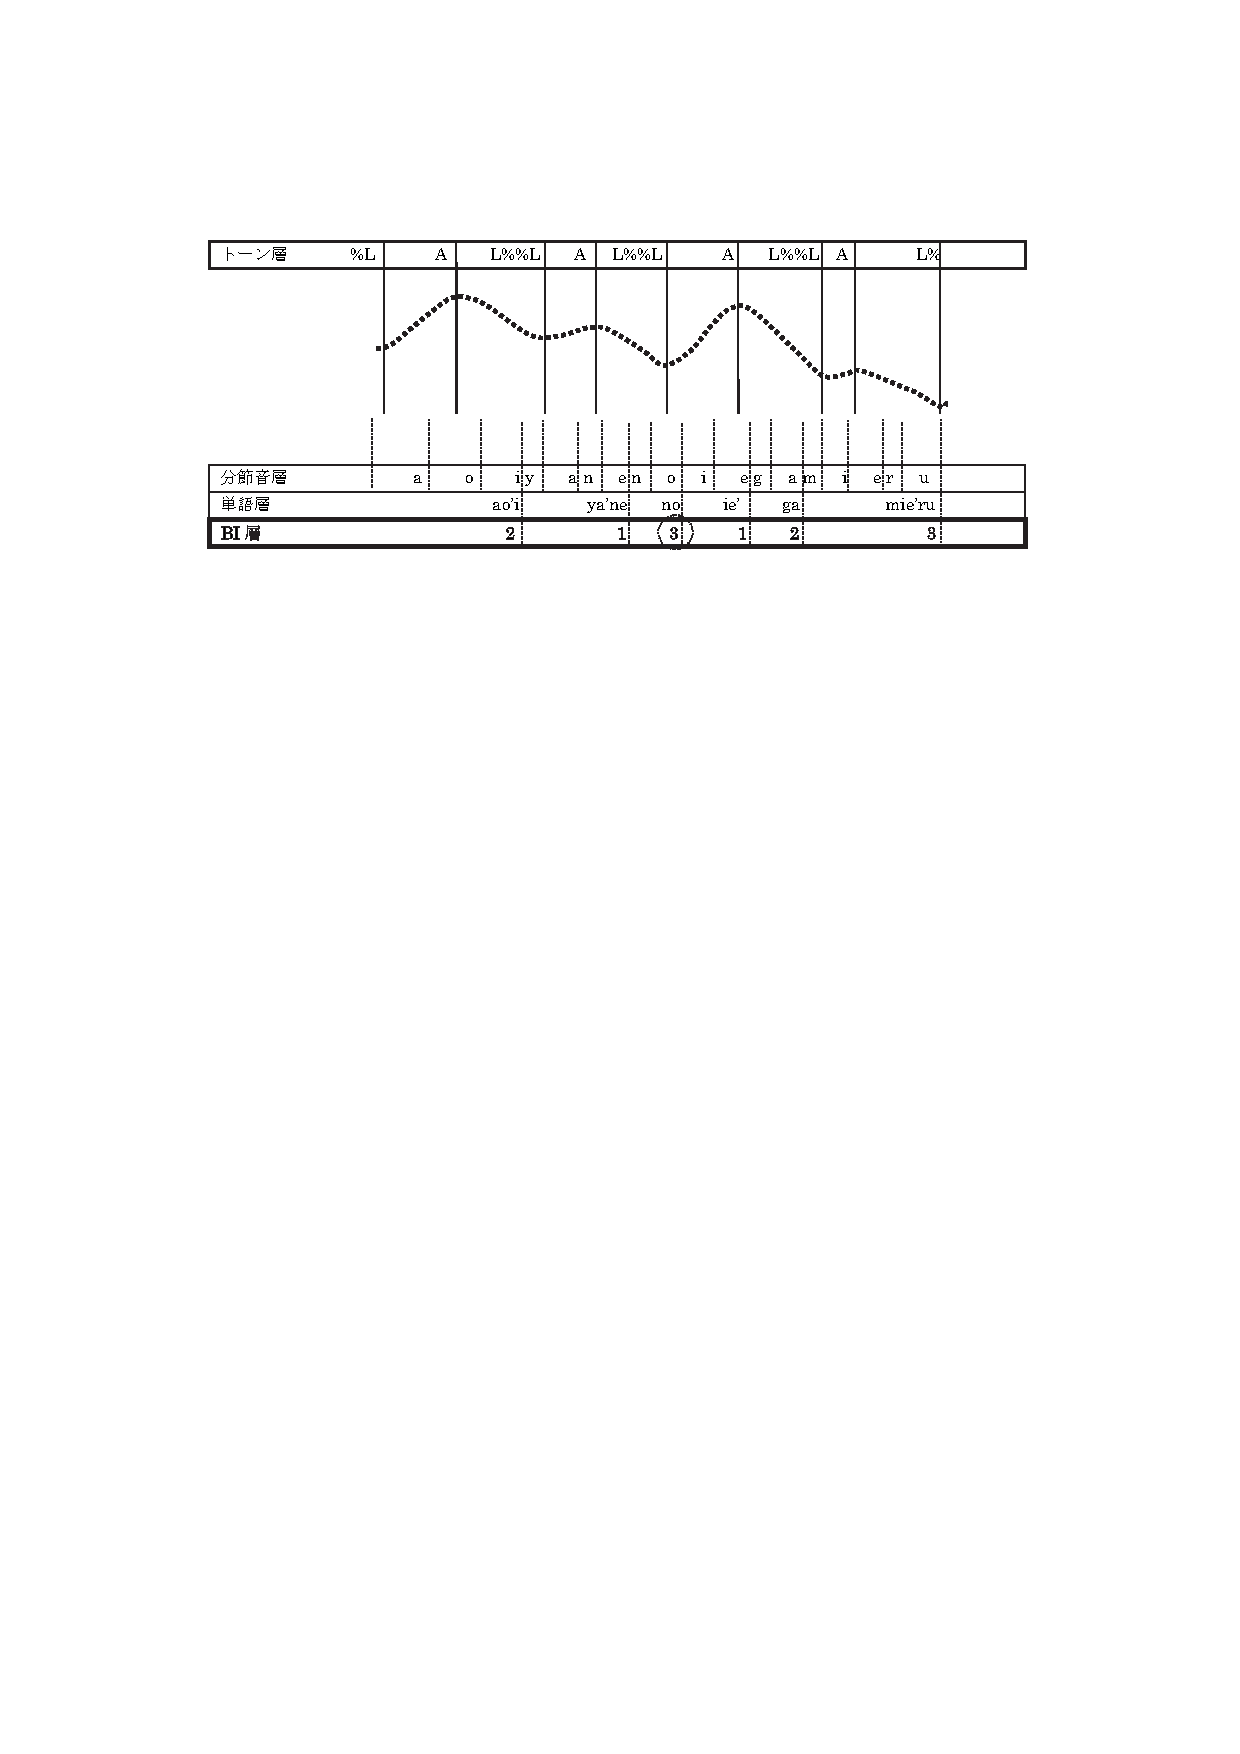
\includegraphics[width=0.7\textwidth]{figure_BIex.pdf}
 \caption{An example of annotation of BI \cite[][412]{igarashietal06}}
 \label{BIexF}
%\end{minipage}
%\end{figure}
%\begin{figure}
%\begin{minipage}{0.5\textwidth}
%\vspace{2cm}
% \centering
% 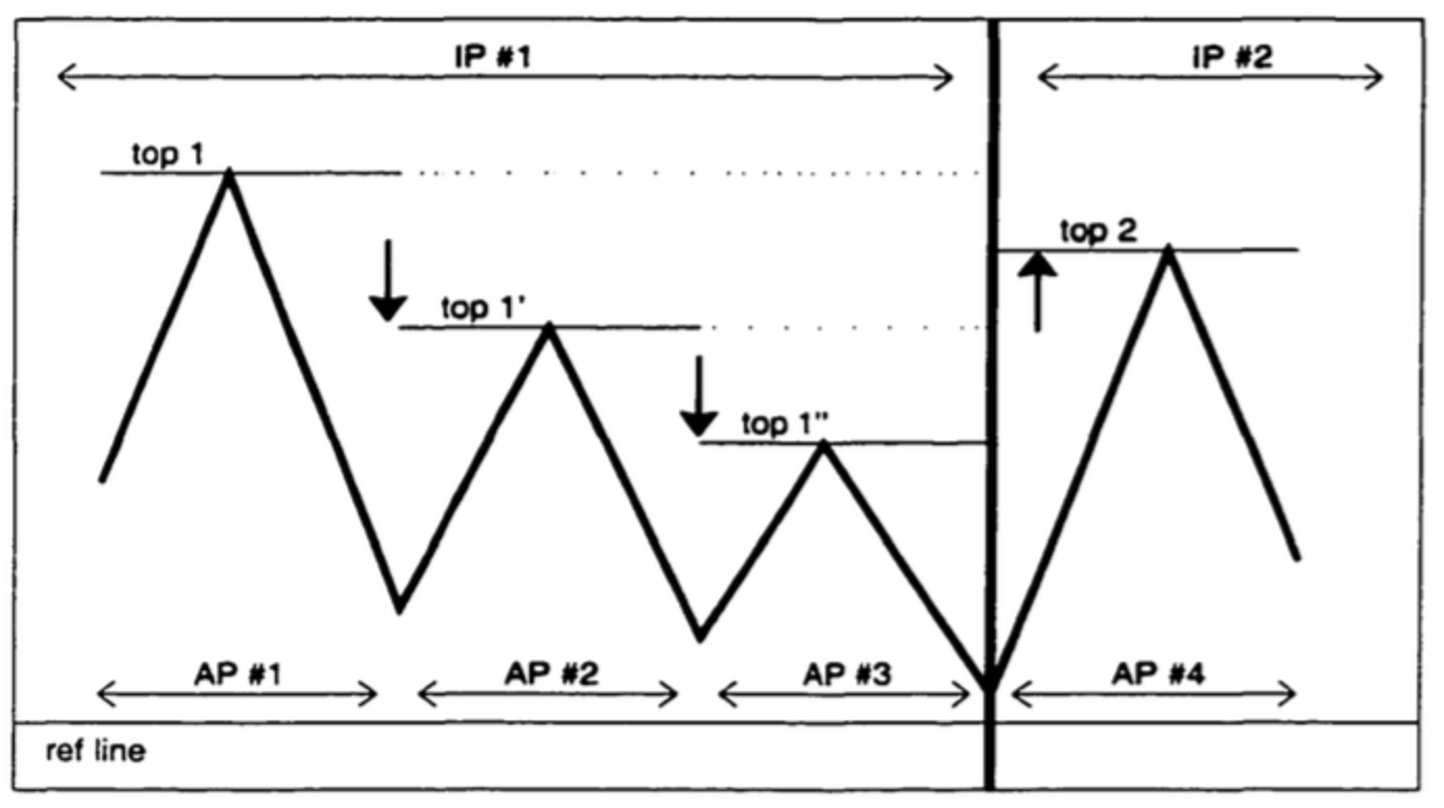
\includegraphics[width=0.5\textwidth]{figure_Venditti00_18.pdf}
% \caption{A schematic representation of down-stepping and intonational-phrase reseting in Japanese \cite[18]{venditti00}}
% \label{FigDownStep}
%\end{minipage}
\end{figure}


%An intonational phrase roughly corresponds to
%an intermediate phrase and utterance in \citeA{pierrehumbertbeckman88},
%and a major phrase and intonational phrase in \citeA{selkirktateishi91}.
%The correspondence is not one-to-one because
%some level in a theory lacks in another theory.
%For example, \citeA{selkirktateishi91} assume three levels above the major phrase (or accentual phrase) as shown in \Next,
%whereas \citeA{pierrehumbertbeckman88} assume no levels between the major phrase (their intermediate phrase) and the utterance.
%In X-JToBI, 
%Pierrehumbert-Beckman's intermediate level and utterance are further integrated into a single level of intonation phrase,
%which means that there is a single level above the accentual phrase.
%The correspondence is summarized as a table in \Next,
%where ``ST91'' indicates \citeA{selkirktateishi91} and
%``PB88'' indicates \citeA{pierrehumbertbeckman88}.%
% \footnote{
% In \citeA{selkirk09}, however, the distinction between
% major vs.~minor phrases is abandoned and only a single level, a phonological phrase, is hypothesized.
% The level of utterance is also dismissed.
% }
%%
%\ex. \EM{Levels of prosody in different theories} \\
%\begin{tabular}{llll}
%\toprule
%   & ST91 & PB88 & X-JToBI \\
%\midrule
% a. & \EM{Utterance} & Utterance & \rdelim\}{3}{1.5in}[Intonational phrase]  \\
% b. & \EM{Intonational phrase} & \rdelim\}{2}{1.5in}[Intermediate phrase] & \\
% c. & \EM{Major phrase} & & \\
% d. & {Minor phrase} & & \\
%    & {(Accentual phrase)} & & \\
% e. & Prosodic word & & \\
% f. & Foot & & \\
% g. & Syllable & & \\
% h. & Mora & & \\
%\bottomrule
%\end{tabular}
%
%What is more complicated is that
%the definition of each level varies depending on theories.
%However, major phrase, intermediate phrase, and intonational phrase basically based on the domain of downstepping.
%The present study is based on X-JToBI because
%this is the only label extensively annotated in a large spoken corpus, namely CSJ.
%However, I leave open the question of whether this label is the best or not.
%I will briefly discuss this issue in Chapter \ref{Intonation}.
%Note that, in reviewing the literature in the following section,
%different theories assume different levels of prosody and
%the definition of each level also varies.

%%----------------------------------------------------
\paragraph{Intonation unit}

Based on X-JToBI,
\citeA{denetal10} and \citeA{denetal11} propose the definition of intonation unit,
which I will employ in this study.
They call it short utterance-unit as opposed to long utterance-unit,
but I use the term ``intonation unit (IU)'' throughout
since I do not discuss long utterance-units.
An intonation-unit boundary is identified
where there is an intonational phrase (the boundary labelled as \code{3} in CSJ) discussed above,
a clause boundary,%
	\footnote{
	To be more precise, this is a long utterance-unit boundary.
	See \citeA{denetal11} for the definition of this unit.
	}
or
a pause equal to or more than 0.1 seconds.
As discussed in \citeA{enomotoetal04},
it is difficult for human annotators to agree in deciding intonation-unit boundaries based on the system proposed in \citeA{duboisetal92} and \citeA{iwasaki08}.
Den and his colleagues made it possible to identify intonation units in spontaneous speech consistently across annotators.

In the following section, however,
I review studies on various kinds of intonation units including those of \citeA{duboisetal92,maekawaetal02,iwasaki08,denetal11}.
Also, whereas prominence marking, down-stepping, and boundary pitch movements are more popular topics than intonation units,
I review those studies in relation to the current study.
See \citeA{vendittietal08} for an overview of such studies.


%%----------------------------------------------------
%\subsubsection{Prominence (pitch peak)}\label{BackSubSubSecProminence}
%
%Focus
%New \& non-adjacent Given elements \cite{venditti00}
%
%%----------------------------------------------------
%\subsubsection{Nonprominence (pitch valley)}\label{BackSubSubSecNonProminence}
%
%Adjacent given elements \cite{venditti00}
%
%%----------------------------------------------------
%\subsubsection{Down-stepping}\label{BackSubSubSecDownStep}





%%----------------------------------------------------
%\subsubsection{Pause}\label{BackSubSubSecPause}

%%% 会話分析による、日本語の話題導入の方法

%%----------------------------------------------------
\subsubsection{Intonation units and related phenomena}

In this section,
I present a review of the literature on the association between prosodic units and related characteristics of language.
Note again that
the review includes various kinds of prosodic units
based on slightly different definitions,
although they agree in many cases.

%%----------------------------------------------------
\paragraph{Prominence and downstepping}

Prominence and downstepping are crucial features in determining intonation units.
It is well known that
a focus receives prominence (pitch peak).
\citeA[99--101]{pierrehumbertbeckman88} report that
``sequences with focus on the noun almost always had an intermediate phrase [i.e., intonational phrase] boundary between the adjective and the noun[...] an intermediate phrase boundary blocks catathesis [i.e., downstepping]'',
through production experiments,
where subjects were asked to produce a sequence of an adjective and a noun with different focus positions.
Target sentences and contexts Pierrehumbert and Beckman used are like the one in \Next.
The capital letters indicate that those words are in focus, and
the bold-faced letters indicate that they are the targets of analysis.
%
%\ex.
% \a.[Q:] [In America,] are there sweet beans like there are in Japan?
% \bg.[A:] mame-wa ari-masu-ga \EM{AMAI} \EM{mame}-wa ari-mase-n \\
%      bean-\ab{top} exist-\ab{plt}-though sweet bean-\ab{top} exist-\ab{plt}-\ab{neg} \\
%      `There are beans, but there aren't SWEET beans.'
%  \b.[]    \hfill{\cite[59]{pierrehumbertbeckman88}}
%
\ex.
 \a.[Q:] [In America,] are there sweet beans or carrots like there are in Japan?
 \bg.[A:] amai {NINZIN}-wa ari-masu-ga \EM{amai} \EM{MAME}-wa ari-mase-n \\
          sweet carrot-\ab{top} exist-\ab{plt}-though sweet bean-\ab{top} exist-\ab{plt}-\ab{neg} \\
      `There are sweet CARROTS, but there aren't sweet BEANS.'
 \b.[]   \hfill{\cite[59]{pierrehumbertbeckman88}}

Pierrehumbert and Beckman showed that
there is an intonational phrase (i.e., intermediate phrase) boundary
between the adjective (\ci{amai} `sweet' in \Last[A]) and the noun (\ci{mame} `bean' in \Last[b])
when the noun is focused as in \Last.
Although the results are complicated,
they conclude that their generalization applies to both accented and unaccented words.%
 \footnote{
 \citeA{kubozono07} compared two definitions of downstepping (syntagmatic and paradigmatic) and investigated whether a pitch reset occurs before the focus.
 He found conflicting results;
 from a syntagmatic perspective, the focus receives higher pitch than the preceding phrase, which indicates that downstepping is blocked.
 From a paradigmatic perspective, on the other hand,
 he had to conclude that downstepping is not blocked before the focus.
 The present study employs the definition of syntagmatic downstepping
 and assumes that the conclusions in \citeA{pierrehumbertbeckman88} and \citeA{kubozono07} do not contradict each other.
 See \citeA{kubozono07} for detailed discussion on this issue.
 }

%%% フォーカスがピッチリセットを引き起こすか(kubozono, PB, Poser)
%%% contrastive focusと普通のフォーカスの音調の違い (郡)


%%----------------------------------------------------
\paragraph{Focus projection}

There has been a cross-linguistic question of how
human beings distinguish broad focus and narrow focus:
the issue of focus projection.
This has been investigated based on English, German and Dutch
\cite{selkirk84,gussenhoven83}.
\citeA{ito02}, who investigated this question in Japanese,
compared the response time and acceptability of each of the intonation types in \Next[A1-A3]
followed by a broad focus question like \Next[Q].
The capital letters indicate the phrases whose pitch range is expanded.
\ex.
 \ag.[Q:] yokoyama-kun-wa boonasu morat-tara doo suru-no \\
          Yokoyama-\ab{hon}-\ab{top} bonus get-\ab{cond} how do-\ab{q} \\
          `What will Mr.Yokoyama do when he gets a bonus?'
 \bg.[A1:] kare-wa \EM{DAIBINGU-o} \EM{HAZIMERU-n-da-yo} \\
           \ab{3}\ab{sg}-\ab{top} diving-\ab{acc} begin-\ab{nmlz}-\ab{cop}-\ab{fp} \\
           `He starts (scuba) diving.'
 \bg.[A2:] kare-wa \EM{DAIBINGU-o} \EM{hazimeru-n-da-yo} \\
           \ab{3}\ab{sg}-\ab{top} diving-\ab{acc} begin-\ab{nmlz}-\ab{cop}-\ab{fp} \\
           `He starts (scuba) diving.'
 \bg.[A3:] kare-wa \EM{daibingu-o} \EM{HAZIMERU-n-da-yo} \\
           \ab{3}\ab{sg}-\ab{top} diving-\ab{acc} begin-\ab{nmlz}-\ab{cop}-\ab{fp} \\
           `He starts (scuba) diving.'
% \ag. kare-wa \EM{ie-o} \EM{kariru-n-da-yo} \\
%      \ab{3}\ab{sg}-\ab{top} house-\ab{acc} rent-\ab{nmlz}-\ab{cop}-\ab{fp} \\
%      `He rents a house'
% \bg. kare-wa \EM{ie-o} {kariru-n-da-yo} \\
%      \ab{3}\ab{sg}-\ab{top} house-\ab{acc} rent-\ab{nmlz}-\ab{cop}-\ab{fp} \\
% \bg. kare-wa {ie-o} \EM{kariru-n-da-yo} \\
%      \ab{3}\ab{sg}-\ab{top} house-\ab{acc} rent-\ab{nmlz}-\ab{cop}-\ab{fp} \\
      \hfill{\cite[412]{ito02}}

Ito found that
``though dual prominence [like \Last[A1]] is preferred for answers to broad focus questions,
utterances with a single intonational prominence on the object [like \Last[A2]] may be comprehended equally quickly as those with dual prominence'' (op.cit.: 413),
whereas A1 is significantly more acceptable than A2.
Also, she reports that the response time and acceptability of the A3-type do not significantly differ from those of A1 and A2.
She concluded that
``it is possible that the relation between argument structure and intonational focus marking is not universal'' (ibid.).

%The results reported in \citeA{kori11}, on the other hand,
%suggest that the intonation of broad and narrow focus is different.
%
\citeA{kori11} investigated intonation of broad and narrow focus and
reports that, by default,
only the first word receives pitch peak and the following word is
suppressed,
although some speakers put prominence on the second word too.
\Next[a] is the target sentence that he asked participants to read aloud
and \Next[b-c] are contexts.
In \Next[b-c], both \ci{aoi} `blue' and \ci{mahuraa} `scarf' are focused
because both of them contrast with `red' and `gloves' or `sweater', respectively.
In \Next[d], \ci{aoi} `blue' is narrowly focused
because only \ci{aoi} `blue' contrasts with `red' and
`scarf' is not contrasted.
%
\ex.
 \ag. \EM{aoi} \EM{mahuraa}-dat-ta-n-desu \\
      blue scarf-\ab{cop}-\ab{past}-\ab{nmlz}-\ab{cop}.\ab{plt} \\
      `(It) was a blue scarf.'
 \b. I ordered \EMi{red gloves}, but I received \EM{a blue scarf}. \hfill{(Broad focus)}
 \b. I ordered \EMi{a red sweater}, but I received \EM{a blue scarf}.\hfill{(Broad focus)}
 \b. I ordered \EMi{a red scarf}, but I received \EM{a blue scarf}. \hfill{(Narrow focus)}

Kori concludes that
the default intonation for broad focus is to suppress the second word (\ci{mahuraa} `scarf' in this case)
because most of the participants produced the sentences as such,
although some participants chose the sentence with prominence both on \ci{aoi} `blue' and \ci{mahuraa} `scarf'
when they were asked to choose a good sentence.

%%%----------------------------------------------------
%\paragraph{Syntactic structure}
%
%\citeA{selkirk09} propose the hypothesis that
%``the clause structure of a sentence in Japanese
%corresponds to a domain for certain of the phonological and phonetic phenomena that contribute to defining the intonational patterns of Japanese sentence.
%This domain has been referred to as the $\iota$-domain, or intonational phrase'' \cite[66]{selkirk09}.
%Selkirk proposes two pieces of evidence that support her hypothesis,
%one of which is from \citeA{kawaharashinya08},
%who investigated the intonation of gapping and coordination in Japanese.
%Here I only introduce the first piece of evidence Selkirk provides
%because the second one seems to me to require further investigations.
%Kawahara and Shinya assume that
%prosodic and syntactic structures have some correspondence
%and explored the associations between them.
%Assuming that there are four levels above the phonological word,
%they hypothesized the correspondence as schematized in \Next.
%%
%\exg.
% {Syntactic boundaries:} $_{Sentence}$[... $_{Clause}$[... $_{VP}$[... {\hspace{0.2cm}} $_{NP}$[... ] ...] ...] ...] \\
% {\it Prosodic boundaries:} Utt IP MaP {\hspace{0.2cm}} MiP \\
% \hfill{\cite[65]{kawaharashinya08}}
%
%In a clause, corresponding to their intonational phrase,
%they found initial rise, pitch reset, final lowering, final pause, and final creakiness.
%In a VP, assumed to correspond to their major phrase,
%they found initial rise and pitch reset,
%both of which are smaller than those of intonational phrases,
%but found no final lowering, final pause, and final creakiness.
%
%%The second piece of evidence for the hypothesis of syntax-phonology correspondence is from \citeA{ishihara02}.
%%\exg. 
%
%%%% 統語構造の曖昧性を韻律で解決する (心理言語学の人たち)
%%%% Kawahara & Shinya (2008): 節頭のpitch riseのほうが節中のpitch riseよりも大きい → intonational phraseの存在。intonational phraseは統語構造と一致している。(Selkirk, 2009)
%%%% Deguchi & Kitagawa (2002); Ishihara (2002): 
%
%Functions of prosody to disambiguate syntactic structures are also well studied in the literature.
%For example,
%\citeA{uyenoetal80} studied how prosody affects the interpretation of syntactically ambiguous sentences like \Next,
%where \ci{ototoi} `the day before yesterday' is ambiguous over
%whether it is included in the relative clause (left-branching interpretation) or in the main clause (center-embedded interpretation).
%They manipulated the pitch peaks of relative clauses
%and had participants listen to the recording and judge whether the sentences are interpreted as left-branching or center-embedded.
%%
%\ex.
% \ag. [\EM{ototoi} koron-da otona]-ga warat-ta \\
%      day.before.yesterday fall-\ab{past} adult-\ab{nom} laugh-\ab{past} \\
%      `The adult who fell the day before yesterday laughed.'
%      \hfill{(Left-branching)}
% \bg. \EM{ototoi} [koron-da otona]-ga warat-ta \\
%      day.before.yesterday fall-\ab{past} adult-\ab{nom} laugh-\ab{past} \\
%      `The adult who fell laughed the day before yesterday.'
%      \hfill{(Center-embedded)}
% \b.[] \hfill{\cite[225]{uyenoetal80}}
%
%They found that
%``[w]hen the pitch assigned to the relative clause is the same or higher than that of the preceding portion of the sentence,
%it tends to be interpreted as center-embedded, otherwise as left-branching'' (op.cit.: 234).

%%----------------------------------------------------
\paragraph{Functional and cognitive motivations for intonation units}

\citeA{iwasaki93},
applying the style of IU identification proposed in \citeA{duboisetal92} and \citeA{chafe94}  to Japanese,
argues that a Japanese intonation unit corresponds to a phrase rather than a clause,
while \citeA{chafe87,chafe94} reports that an English IU often corresponds to a clause.
According to Iwasaki's survey,
clausal IUs in Japanese are 42.2\%,
whereas phrasal IUs are 57.8\%.
Their intonation unit is a ``stretch of speech uttered under a single coherent intonation contour'' \cite[17]{duboisetal92}.
\citeA[39]{iwasaki93} states that
the beginning of an IU ``is often, though not always, marked by a pause, hesitation noises, and/or resetting of the baseline pitch level'',
whereas the ending of an IU ``is often, again though not always, marked by a lengthening of the last syllable.''
\citeA{iwasaki93} provides \Next as an example of intonation units in Japanese corresponding to a phrase.
Each line in \Next corresponds to a single intonation unit
and \Next[a-e] as a whole consist of a single proposition
``I heard that broadcast at home with my family.''
%
\ex.
 \ag. atasi-wa-ne:* \\
      \ab{1}\ab{sg}-\ab{top}-\ab{fp} \\
      `I, you know...'
 \bg. uti-de kii-ta-no-ne? \\
      home-\ab{loc} hear-\ab{past}-\ab{nmlz}-\ab{fp} \\
      `heard at home, you know...'
 \bg. sono are-wa-ne? \\
      that that-\ab{top}-\ab{fp} \\
      `that thing, you know...'
 \bg. hoosoo-wa-ne? \\
      broadcast-\ab{top}-\ab{fp} \\
      `that broadcast, you know,'
 \bg. kazoku-de. \\
      family-with \\
      `with my family.'
 \hfill{\cite[40]{iwasaki93}}

The pitch and intensity of \Next are shown in Figure \ref{IUExF} from
\citeA[109]{iwasaki08},
where he explains the same example with the figure.
The IU \Next[a] ends with a final vowel lengthening,
whereas boundary pitch movements are observed in the ending of IUs \Next[b-d],
which are indicated by ``?''.
\Next[e] ends with a final lowering, indicated by ``.''.

Iwasaki divided the kinds of ``functional components'' into four types.
%
\ex.
 \tl{Four functional components}
 \a. \EM{Lead (LD)} such as fillers, which have no substantial meaning
 \b. \EM{Ideation (ID)}, which conveys the content of speech
 \b. \EM{Cohesion (CO)} such as conjunctives and \ci{wa}, which relates the previous and the current IUs
 \b. \EM{Interaction (IT)} such as \ci{ne} `\ab{fp}' and \ci{yo} `\ab{fp}', which is associated with communication

Based on this,
he showed the similarities among IUs.
For example, 
\Next[a] is an IU which only contains an NP followed by particles, and
\Next[b] is an IU which only contains a VP also followed by particles.
%According to the functional component classification in \Last,
The structures of these two IUs are essentially the same in terms of functional components,
although they are different in terms of grammatical structure.
%
\ex.
 \a.
  \glll [mami-ni-dake] [-wa] [-ne] \\
        Mami-\ab{dat}-only -\ab{top} -\ab{fp} \\
        \EM{ID} \EM{CO} \EM{IT} \\
 \b.
  \glll [ik-ase-ta-rasii] [-no] [-yo] \\
         go-\ab{caus}-\ab{rep} -\ab{nmlz} -\ab{fp} \\
         \EM{ID} \EM{CO} \EM{IT} \\
  \glt  `(I heard that she) let only Mami go.'
% \a.
% \glll [sooyuu sito-ga siki si] [-te] [-ne*] \\
%       such person-\ab{nom} lead do -and -\ab{fp} \\
%       \EM{ID} {} {} {} \EM{CO} \EM{IT} \\
% \glt `Such people led and...'
% \b.
% \glll [sinin-o asoko-e minnna] [-ne*] \\
%        corpse-\ab{acc} there-\ab{gl} all -\ab{fp} \\
%        \EM{ID} {} {} \EM{IT} \\
% \glt   `all the corpses to there...'
% \b.
% \glll [ano] [dote-no ue-e] [-sa*] \\
%       \ab{fl} bank-\ab{gen} top-\ab{gl} -\ab{fp} \\
%       \EM{LD} \EM{ID} {} \EM{IT} \\
% \glt  `to the top of the bank...'
% \b.
% \glll [atume] [-te.] \\
%      gather and \\
%      \EM{ID} \EM{CO} \\
% \glt `gathered and...'
% \hfill{\cite[47]{iwasaki93}}

Iwasaki analyzed his data based on his classification and
found that more than 80\% of the IUs consist of
two or less functional components.
He states that
``this might be due to the limitation of work that the speaker can handle within one IU. [...] Japanese speakers [...] are faced with a constraint which permits them to exercise up to two functions per intonation unit'' (p.~49).


\begin{figure}
 \centering
 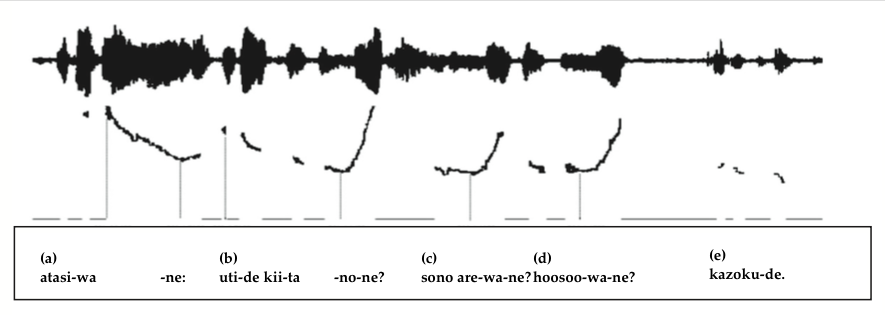
\includegraphics[width=0.85\textwidth]{sounds/iwasaki_IU.png}
 \caption{An example of an intonation unit \cite[109]{iwasaki08}}
 \label{IUExF}
\end{figure}


On the contrary, \citeA[68]{matsumoto00} reports that
``one clause comprises an average of 1.2 IUs''
and argues that
``the clause is the syntactic exponent of Japanese substantive IU''.
Instead, she proposes the ``one new NP per IU'' constraint in Japanese,
comparing it to the one new idea at a time constraint in \citeA{chafe87,chafe94}.
However, \citeA[\S 5.6]{matsumoto03} also reports that
one new or given NP per IU is preferred in Japanese conversation.
Therefore,
new as well as given NPs appear in an intonation unit
without other NPs.
%although she proposes ``one new NP per IU'' constraint
%also in this paper.


%\citeA{matsumoto03} extensively investigates the association between
%intonation units and syntactic structure, information structure, and functional structure.
%Here I review her study focusing on the association between
%intonation units and information structure.

%%%\citeA{sakutafujii}

\citeA{nakagawaetal10_piu} focused on the difference between
phrasal IUs and clausal IUs and
analyzed them in terms of information structure.
They measured referential distance and persistence \cite{givon83} and concluded that
one of the functions of phrasal IUs is to introduce or re-introduce
important topics in discourse.
They compare this function of phrasal IUs to left-dislocations observed in many languages.

%%----------------------------------------------------
%\paragraph{Other factors}
%
%length of a unit % \citeA{ghini93}
%speech rate % \citeA{hayeslahiri91}



%%----------------------------------------------------
\paragraph{Remaining issues}

Most studies on phonetics and phonology concentrate on
foci rather than topics.
Among foci, most of the studies (except for those on focus projection) concentrate on narrow focus rather than broad focus.
Moreover, almost all of them are experimental studies rather than
corpus studies.
On the other hand, I focus here on
the difference between broad foci and topics in spontaneous speech,
although I also employ a production experiment.

Functionalists such as \citeA{iwasaki93,matsumoto00,matsumoto03} and \citeA{nakagawaetal10_piu}
have methodological issues since they rely on the impressionistic definition of intonation units.
This study, on the contrary, is based on
strict definitions of intonation units and
aims at revealing associations between intonation and information structure.

The results in Chapter \ref{Intonation} show that
an intonation unit corresponds to a unit of information structure such as topic and focus,
which frequently but not always overlaps with a unit of syntactic structure.

%%----------------------------------------------------
\subsubsection{Pause}

\citeA{sugito94} showed that
pauses appear before pitch reset by means of a perceptual experiment.
She recorded trained announcers reading news and had subjects listen to the recording.
She found that, when pauses were eliminated,
subjects perceive the voice as though two people were overlapping with each other where there are pitch resets and there are supposed to be pauses.
According to her,
it is in fact impossible to reset pitch without pauses and
vocal cords are tensed 0.1 seconds before speech production.
Therefore, I assume that pauses correlate with pitch reset.

%%----------------------------------------------------
%%----------------------------------------------------
\section{Summary}

In this chapter,
I outlined the previous literature on topics and foci, and
the characteristics of Japanese related to this study,
and enumerated the remaining questions to be investigated.

In Chapters from \ref{Particles} to \ref{Intonation},
I investigate the associations between information structure and particles, word order, and intonation in spoken Japanese.
Before this,
I introduce the framework this study employs in the next chapter.




